\documentclass[twoside]{book}

% Packages required by doxygen
\usepackage{calc}
\usepackage{doxygen}
\usepackage{graphicx}
\usepackage[utf8]{inputenc}
\usepackage{makeidx}
\usepackage{multicol}
\usepackage{multirow}
\usepackage{textcomp}
\usepackage[table]{xcolor}

% NLS support packages
\usepackage{polski}
\usepackage[T1]{fontenc}

% Font selection
\usepackage[T1]{fontenc}
\usepackage{mathptmx}
\usepackage[scaled=.90]{helvet}
\usepackage{courier}
\usepackage{amssymb}
\usepackage{sectsty}
\renewcommand{\familydefault}{\sfdefault}
\allsectionsfont{%
  \fontseries{bc}\selectfont%
  \color{darkgray}%
}
\renewcommand{\DoxyLabelFont}{%
  \fontseries{bc}\selectfont%
  \color{darkgray}%
}

% Page & text layout
\usepackage{geometry}
\geometry{%
  a4paper,%
  top=2.5cm,%
  bottom=2.5cm,%
  left=2.5cm,%
  right=2.5cm%
}
\tolerance=750
\hfuzz=15pt
\hbadness=750
\setlength{\emergencystretch}{15pt}
\setlength{\parindent}{0cm}
\setlength{\parskip}{0.2cm}
\makeatletter
\renewcommand{\paragraph}{%
  \@startsection{paragraph}{4}{0ex}{-1.0ex}{1.0ex}{%
    \normalfont\normalsize\bfseries\SS@parafont%
  }%
}
\renewcommand{\subparagraph}{%
  \@startsection{subparagraph}{5}{0ex}{-1.0ex}{1.0ex}{%
    \normalfont\normalsize\bfseries\SS@subparafont%
  }%
}
\makeatother

% Headers & footers
\usepackage{fancyhdr}
\pagestyle{fancyplain}
\fancyhead[LE]{\fancyplain{}{\bfseries\thepage}}
\fancyhead[CE]{\fancyplain{}{}}
\fancyhead[RE]{\fancyplain{}{\bfseries\leftmark}}
\fancyhead[LO]{\fancyplain{}{\bfseries\rightmark}}
\fancyhead[CO]{\fancyplain{}{}}
\fancyhead[RO]{\fancyplain{}{\bfseries\thepage}}
\fancyfoot[LE]{\fancyplain{}{}}
\fancyfoot[CE]{\fancyplain{}{}}
\fancyfoot[RE]{\fancyplain{}{\bfseries\scriptsize Wygenerowano Cz, 21 maj 2015 00\-:15\-:04 dla lab8 programem Doxygen }}
\fancyfoot[LO]{\fancyplain{}{\bfseries\scriptsize Wygenerowano Cz, 21 maj 2015 00\-:15\-:04 dla lab8 programem Doxygen }}
\fancyfoot[CO]{\fancyplain{}{}}
\fancyfoot[RO]{\fancyplain{}{}}
\renewcommand{\footrulewidth}{0.4pt}
\renewcommand{\chaptermark}[1]{%
  \markboth{#1}{}%
}
\renewcommand{\sectionmark}[1]{%
  \markright{\thesection\ #1}%
}

% Indices & bibliography
\usepackage{natbib}
\usepackage[titles]{tocloft}
\setcounter{tocdepth}{3}
\setcounter{secnumdepth}{5}
\makeindex

% Hyperlinks (required, but should be loaded last)
\usepackage{ifpdf}
\ifpdf
  \usepackage[pdftex,pagebackref=true]{hyperref}
\else
  \usepackage[ps2pdf,pagebackref=true]{hyperref}
\fi
\hypersetup{%
  colorlinks=true,%
  linkcolor=blue,%
  citecolor=blue,%
  unicode%
}

% Custom commands
\newcommand{\clearemptydoublepage}{%
  \newpage{\pagestyle{empty}\cleardoublepage}%
}


%===== C O N T E N T S =====

\begin{document}

% Titlepage & ToC
\hypersetup{pageanchor=false}
\pagenumbering{roman}
\begin{titlepage}
\vspace*{7cm}
\begin{center}%
{\Large lab8 \\[1ex]\large 0.\-0008 }\\
\vspace*{1cm}
{\large Wygenerowano przez Doxygen 1.8.6}\\
\vspace*{0.5cm}
{\small Cz, 21 maj 2015 00:15:04}\\
\end{center}
\end{titlepage}
\clearemptydoublepage
\tableofcontents
\clearemptydoublepage
\pagenumbering{arabic}
\hypersetup{pageanchor=true}

%--- Begin generated contents ---
\chapter{Laboratorium 8}
\label{index}\hypertarget{index}{}\begin{DoxyAuthor}{Autor}
Filip Malinowski 
\end{DoxyAuthor}
\begin{DoxyDate}{Data}
22.\-04.\-2015 
\end{DoxyDate}
\begin{DoxyVersion}{Wersja}
0.\-0005
\end{DoxyVersion}
Program sluzacy do uruchamiania algorytmow i badania ich szybkosci dzialania.\par
W programie zaimplementowane sa algorytmy\-:\par

\begin{DoxyItemize}
\item sortowania szybkiego stosu\par

\item sortowania szybkiego po optymalizacji pivot stosu\par

\item sortowania przez scalanie stosu\par

\item sortowania przez kopcowanie stosu
\end{DoxyItemize}

Do wykonania podanych powyzej trzech ostatnich algorytmow zostaly zaimplementowane potrzebne struktury danych (stos, kolejka, lista oraz lista tablicowa, lista asocjacyjna, tablica z haszowaniem).\par
\par
Ciala klas znajduja sie w folderze ./prj/inc\par
Definicje metod znajduja sie w folderze ./prj/src\par
Sprawozdanie znajduje sie w folderze ./prj/doc/sprawozdanie\par
\par
Format wywolania\-:\par

\begin{DoxyCode}
./prj/make clean\(\backslash\)n
./prj/make\(\backslash\)n
\end{DoxyCode}
 
\chapter{Indeks hierarchiczny}
\section{Hierarchia klas}
Ta lista dziedziczenia posortowana jest z grubsza, choć nie całkowicie, alfabetycznie\-:\begin{DoxyCompactList}
\item \contentsline{section}{Benchmark}{\pageref{class_benchmark}}{}
\begin{DoxyCompactList}
\item \contentsline{section}{Mnozenie}{\pageref{class_mnozenie}}{}
\end{DoxyCompactList}
\end{DoxyCompactList}

\chapter{Indeks klas}
\section{Lista klas}
Tutaj znajdują się klasy, struktury, unie i interfejsy wraz z ich krótkimi opisami\-:\begin{DoxyCompactList}
\item\contentsline{section}{\hyperlink{class_algorithm_kolejka}{Algorithm\-Kolejka} \\*Klasa \hyperlink{class_algorithm_kolejka}{Algorithm\-Kolejka} modelujaca algorytm wczytywania do kolejki. Obiekt tego typu reprezentuje algorytm wykonujacy wykonujacy wczytywanie zadanej ilosci elementow do kolejki }{\pageref{class_algorithm_kolejka}}{}
\item\contentsline{section}{\hyperlink{class_algorithm_lista}{Algorithm\-Lista} \\*Klasa \hyperlink{class_algorithm_lista}{Algorithm\-Lista} modelujaca algorytm wczytywania do kolejki. Obiekt tego typu reprezentuje algorytm wykonujacy wykonujacy wczytywanie zadanej ilosci elementow do listy }{\pageref{class_algorithm_lista}}{}
\item\contentsline{section}{\hyperlink{class_algorithm_stos}{Algorithm\-Stos} \\*Klasa \hyperlink{class_algorithm_stos}{Algorithm\-Stos} modelujaca algorytm wczytywania do stosu. Obiekt tego typu reprezentuje algorytm wykonujacy wykonujacy wczytywanie zadanej ilosci elementow do stosu }{\pageref{class_algorithm_stos}}{}
\item\contentsline{section}{\hyperlink{class_benchmark}{Benchmark} \\*Klasa \hyperlink{class_benchmark}{Benchmark} modelujaca program benchmarkujacy. Obiekt tego typu reprezentuje program sprawdzajacy szybkosc wykonywania algorytmow }{\pageref{class_benchmark}}{}
\item\contentsline{section}{\hyperlink{class_kolejka}{Kolejka} \\*Klasa \hyperlink{class_kolejka}{Kolejka} modelujaca strukture danych typu kolejka. Obiekt tego typu reprezentuje strukture danych typu kolejka wraz z operacjami mozliwymi do wykonania na tej strukturze }{\pageref{class_kolejka}}{}
\item\contentsline{section}{\hyperlink{struct_lista_1_1_komorka}{Lista\-::\-Komorka} \\*Struktura \hyperlink{struct_lista_1_1_komorka}{Komorka}. Obiekt tego typu reprezentuje pojedyncza komorke wraz ze wskaznikiem na nastepna komorke listy }{\pageref{struct_lista_1_1_komorka}}{}
\item\contentsline{section}{\hyperlink{class_lista}{Lista} \\*Klasa \hyperlink{class_lista}{Lista} modelujaca strukture danych typu lista. Obiekt tego typu reprezentuje strukture danych typu lista wraz z operacjami mozliwymi do wykonania na tej strukturze }{\pageref{class_lista}}{}
\item\contentsline{section}{\hyperlink{class_mnozenie}{Mnozenie} \\*Klasa \hyperlink{class_mnozenie}{Mnozenie} modelujaca algorytm mnozenia. Obiekt tego typu reprezentuje algorytm wykonujacy dzialanie mnozenia kazdego elementu tablicy tab przez 2 }{\pageref{class_mnozenie}}{}
\item\contentsline{section}{\hyperlink{class_stos}{Stos} \\*Klasa \hyperlink{class_stos}{Stos} modelujaca strukture danych typu stos. Obiekt tego typu reprezentuje strukture danych typu stos wraz z operacjami mozliwymi do wykonania na tej strukturze }{\pageref{class_stos}}{}
\end{DoxyCompactList}

\chapter{Indeks plików}
\section{Lista plików}
Tutaj znajduje się lista wszystkich plików z ich krótkimi opisami\-:\begin{DoxyCompactList}
\item\contentsline{section}{\hyperlink{algorithm2_8cpp}{algorithm2.\-cpp} }{\pageref{algorithm2_8cpp}}{}
\item\contentsline{section}{\hyperlink{algorithm2_8hh}{algorithm2.\-hh} }{\pageref{algorithm2_8hh}}{}
\item\contentsline{section}{\hyperlink{algorithm__kolejka_8cpp}{algorithm\-\_\-kolejka.\-cpp} }{\pageref{algorithm__kolejka_8cpp}}{}
\item\contentsline{section}{\hyperlink{algorithm__kolejka_8hh}{algorithm\-\_\-kolejka.\-hh} }{\pageref{algorithm__kolejka_8hh}}{}
\item\contentsline{section}{\hyperlink{algorithm__lista_8cpp}{algorithm\-\_\-lista.\-cpp} }{\pageref{algorithm__lista_8cpp}}{}
\item\contentsline{section}{\hyperlink{algorithm__lista_8hh}{algorithm\-\_\-lista.\-hh} }{\pageref{algorithm__lista_8hh}}{}
\item\contentsline{section}{\hyperlink{algorithm__stos_8cpp}{algorithm\-\_\-stos.\-cpp} }{\pageref{algorithm__stos_8cpp}}{}
\item\contentsline{section}{\hyperlink{algorithm__stos_8hh}{algorithm\-\_\-stos.\-hh} }{\pageref{algorithm__stos_8hh}}{}
\item\contentsline{section}{\hyperlink{benchmark_8cpp}{benchmark.\-cpp} }{\pageref{benchmark_8cpp}}{}
\item\contentsline{section}{\hyperlink{benchmark_8hh}{benchmark.\-hh} }{\pageref{benchmark_8hh}}{}
\item\contentsline{section}{\hyperlink{generate_8cpp}{generate.\-cpp} }{\pageref{generate_8cpp}}{}
\item\contentsline{section}{\hyperlink{kolejka_8cpp}{kolejka.\-cpp} }{\pageref{kolejka_8cpp}}{}
\item\contentsline{section}{\hyperlink{kolejka_8hh}{kolejka.\-hh} }{\pageref{kolejka_8hh}}{}
\item\contentsline{section}{\hyperlink{lista_8cpp}{lista.\-cpp} }{\pageref{lista_8cpp}}{}
\item\contentsline{section}{\hyperlink{lista_8hh}{lista.\-hh} }{\pageref{lista_8hh}}{}
\item\contentsline{section}{\hyperlink{main_8cpp}{main.\-cpp} }{\pageref{main_8cpp}}{}
\item\contentsline{section}{\hyperlink{stos_8cpp}{stos.\-cpp} }{\pageref{stos_8cpp}}{}
\item\contentsline{section}{\hyperlink{stos_8hh}{stos.\-hh} }{\pageref{stos_8hh}}{}
\item\contentsline{section}{\hyperlink{tab__lista_8cpp}{tab\-\_\-lista.\-cpp} }{\pageref{tab__lista_8cpp}}{}
\item\contentsline{section}{\hyperlink{tab__lista_8hh}{tab\-\_\-lista.\-hh} }{\pageref{tab__lista_8hh}}{}
\end{DoxyCompactList}

\chapter{Dokumentacja klas}
\hypertarget{class_algorithm1}{\section{Dokumentacja klasy Algorithm1}
\label{class_algorithm1}\index{Algorithm1@{Algorithm1}}
}


Klasa \hyperlink{class_algorithm1}{Algorithm1} modelujaca algorytm sortowania stosu. Obiekt tego typu reprezentuje algorytm wykonujacy sortowanie szybkie na elementach stosu.  




{\ttfamily \#include $<$algorithm1.\-hh$>$}



Diagram dziedziczenia dla Algorithm1\nopagebreak
\begin{figure}[H]
\begin{center}
\leavevmode
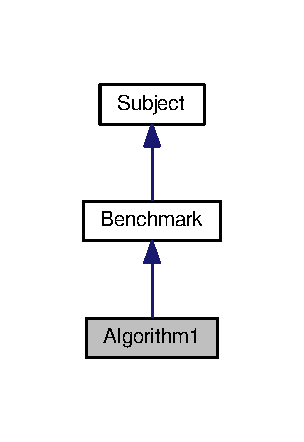
\includegraphics[width=146pt]{class_algorithm1__inherit__graph}
\end{center}
\end{figure}


Diagram współpracy dla Algorithm1\-:\nopagebreak
\begin{figure}[H]
\begin{center}
\leavevmode
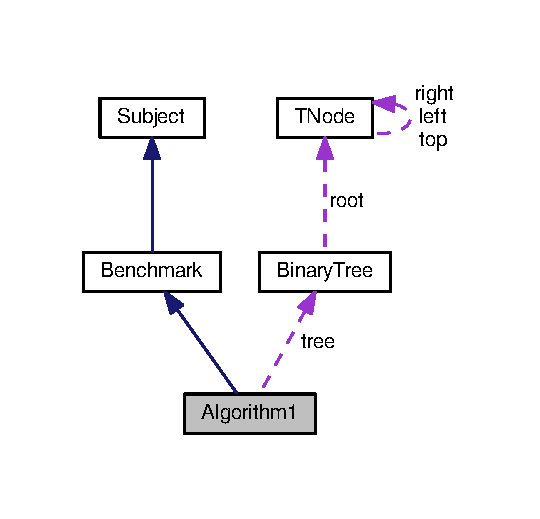
\includegraphics[width=201pt]{class_algorithm1__coll__graph}
\end{center}
\end{figure}
\subsection*{Metody publiczne}
\begin{DoxyCompactItemize}
\item 
\hyperlink{class_algorithm1_ad2b1593378788a36b954b65d1c2af8ff}{Algorithm1} ()
\begin{DoxyCompactList}\small\item\em Konstruktor obiektu \hyperlink{class_algorithm1}{Algorithm1}. \end{DoxyCompactList}\item 
\hyperlink{class_algorithm1_ad2976b6058bd8886cfd20307e79b6042}{Algorithm1} (int $\ast$\-\_\-tab)
\begin{DoxyCompactList}\small\item\em Konstruktor parametryczny obiektu \hyperlink{class_algorithm1}{Algorithm1}. \end{DoxyCompactList}\item 
\hyperlink{class_algorithm1_afbd4d69811879472fcadb25a1c3c5262}{$\sim$\-Algorithm1} ()
\begin{DoxyCompactList}\small\item\em Destruktor obiektu \hyperlink{class_algorithm1}{Algorithm1}. \end{DoxyCompactList}\item 
virtual void \hyperlink{class_algorithm1_a35260610f8093c3812a6f146147955e6}{test\-Algorithm} (\hyperlink{class_benchmark}{Benchmark} $\ast$\-\_\-algorithm)
\begin{DoxyCompactList}\small\item\em Metoda testowania algorytmu. Metoda sluzy do testowania szybkosci dzialania algorytmu. W klasie \hyperlink{class_algorithm1}{Algorithm1} nie ma konkretnego dzialania. \end{DoxyCompactList}\item 
virtual void \hyperlink{class_algorithm1_a008c8fdd07c39219099afe14e63e447a}{load} (int \-\_\-border)
\begin{DoxyCompactList}\small\item\em Metoda przygotowywania algorytmu. Metoda sluzy do przygotowania warunkow do przeprowadzenia testu. \end{DoxyCompactList}\item 
virtual void \hyperlink{class_algorithm1_a135dd26c6c741812d75cd7f2f270592d}{unload} (int \-\_\-border)
\begin{DoxyCompactList}\small\item\em Metoda sprzatania. Metoda sluzy do oproznienia struktury. \end{DoxyCompactList}\item 
virtual void \hyperlink{class_algorithm1_a671a2162843b588704044420c9a5dfa9}{run\-Algorithm} (int \-\_\-border)
\begin{DoxyCompactList}\small\item\em Metoda uruchamiania algorytmu. Metoda sluzy do wykonywania danego algorytmu. Sortuje elementy stosu. \end{DoxyCompactList}\end{DoxyCompactItemize}
\subsection*{Atrybuty prywatne}
\begin{DoxyCompactItemize}
\item 
int $\ast$ \hyperlink{class_algorithm1_a696e1e45bff4a0510dfb76274321583f}{tab}
\begin{DoxyCompactList}\small\item\em Wskaznik na tablice elementow z danymi wejsciowymi. \end{DoxyCompactList}\item 
\hyperlink{class_stos}{Stos} \hyperlink{class_algorithm1_a3fb7f66d1e4aae77a49c6f7c241f47c9}{stos}
\begin{DoxyCompactList}\small\item\em Zmienna przechowujaca stos. \end{DoxyCompactList}\end{DoxyCompactItemize}


\subsection{Opis szczegółowy}


Definicja w linii 9 pliku algorithm1.\-hh.



\subsection{Dokumentacja konstruktora i destruktora}
\hypertarget{class_algorithm1_ad2b1593378788a36b954b65d1c2af8ff}{\index{Algorithm1@{Algorithm1}!Algorithm1@{Algorithm1}}
\index{Algorithm1@{Algorithm1}!Algorithm1@{Algorithm1}}
\subsubsection[{Algorithm1}]{\setlength{\rightskip}{0pt plus 5cm}Algorithm1\-::\-Algorithm1 (
\begin{DoxyParamCaption}
{}
\end{DoxyParamCaption}
)\hspace{0.3cm}{\ttfamily [inline]}}}\label{class_algorithm1_ad2b1593378788a36b954b65d1c2af8ff}


Definicja w linii 24 pliku algorithm1.\-hh.

\hypertarget{class_algorithm1_ad2976b6058bd8886cfd20307e79b6042}{\index{Algorithm1@{Algorithm1}!Algorithm1@{Algorithm1}}
\index{Algorithm1@{Algorithm1}!Algorithm1@{Algorithm1}}
\subsubsection[{Algorithm1}]{\setlength{\rightskip}{0pt plus 5cm}Algorithm1\-::\-Algorithm1 (
\begin{DoxyParamCaption}
\item[{int $\ast$}]{\-\_\-tab}
\end{DoxyParamCaption}
)\hspace{0.3cm}{\ttfamily [inline]}}}\label{class_algorithm1_ad2976b6058bd8886cfd20307e79b6042}

\begin{DoxyParams}[1]{Parametry}
\mbox{\tt in}  & {\em \-\_\-tab} & -\/ tablica przechowujaca dane wejsciowe. \\
\hline
\end{DoxyParams}


Definicja w linii 30 pliku algorithm1.\-hh.

\hypertarget{class_algorithm1_afbd4d69811879472fcadb25a1c3c5262}{\index{Algorithm1@{Algorithm1}!$\sim$\-Algorithm1@{$\sim$\-Algorithm1}}
\index{$\sim$\-Algorithm1@{$\sim$\-Algorithm1}!Algorithm1@{Algorithm1}}
\subsubsection[{$\sim$\-Algorithm1}]{\setlength{\rightskip}{0pt plus 5cm}Algorithm1\-::$\sim$\-Algorithm1 (
\begin{DoxyParamCaption}
{}
\end{DoxyParamCaption}
)\hspace{0.3cm}{\ttfamily [inline]}}}\label{class_algorithm1_afbd4d69811879472fcadb25a1c3c5262}


Definicja w linii 35 pliku algorithm1.\-hh.



\subsection{Dokumentacja funkcji składowych}
\hypertarget{class_algorithm1_a008c8fdd07c39219099afe14e63e447a}{\index{Algorithm1@{Algorithm1}!load@{load}}
\index{load@{load}!Algorithm1@{Algorithm1}}
\subsubsection[{load}]{\setlength{\rightskip}{0pt plus 5cm}void Algorithm1\-::load (
\begin{DoxyParamCaption}
\item[{int}]{\-\_\-border}
\end{DoxyParamCaption}
)\hspace{0.3cm}{\ttfamily [virtual]}}}\label{class_algorithm1_a008c8fdd07c39219099afe14e63e447a}

\begin{DoxyParams}[1]{Parametry}
\mbox{\tt in}  & {\em \-\_\-border} & -\/ ilosc elementow dla ktorych metoda ma wykonac swoje dzialanie. \\
\hline
\end{DoxyParams}


Reimplementowana z \hyperlink{class_benchmark_a935c57201a5d0b9589a898df38b8b5a3}{Benchmark}.



Definicja w linii 15 pliku algorithm1.\-cpp.



Oto graf wywołań dla tej funkcji\-:\nopagebreak
\begin{figure}[H]
\begin{center}
\leavevmode
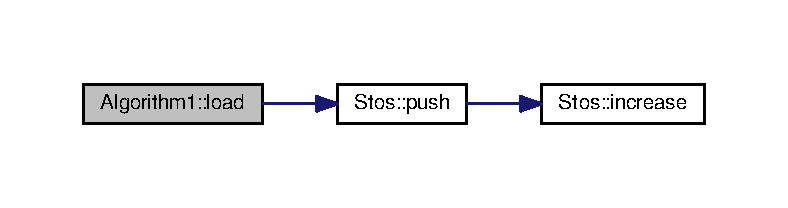
\includegraphics[width=350pt]{class_algorithm1_a008c8fdd07c39219099afe14e63e447a_cgraph}
\end{center}
\end{figure}


\hypertarget{class_algorithm1_a671a2162843b588704044420c9a5dfa9}{\index{Algorithm1@{Algorithm1}!run\-Algorithm@{run\-Algorithm}}
\index{run\-Algorithm@{run\-Algorithm}!Algorithm1@{Algorithm1}}
\subsubsection[{run\-Algorithm}]{\setlength{\rightskip}{0pt plus 5cm}void Algorithm1\-::run\-Algorithm (
\begin{DoxyParamCaption}
\item[{int}]{\-\_\-border}
\end{DoxyParamCaption}
)\hspace{0.3cm}{\ttfamily [virtual]}}}\label{class_algorithm1_a671a2162843b588704044420c9a5dfa9}

\begin{DoxyParams}[1]{Parametry}
\mbox{\tt in}  & {\em \-\_\-border} & -\/ ilosc elementow dla ktorych algorytm ma wykonac swoje dzialanie. \\
\hline
\end{DoxyParams}


Reimplementowana z \hyperlink{class_benchmark_a6363894c058e8bfe146de09d7126b29c}{Benchmark}.



Definicja w linii 9 pliku algorithm1.\-cpp.



Oto graf wywołań dla tej funkcji\-:\nopagebreak
\begin{figure}[H]
\begin{center}
\leavevmode
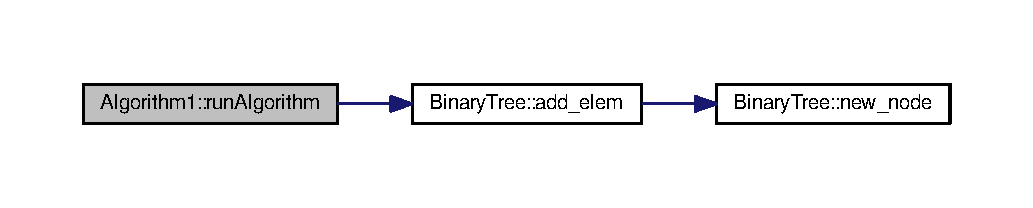
\includegraphics[width=320pt]{class_algorithm1_a671a2162843b588704044420c9a5dfa9_cgraph}
\end{center}
\end{figure}


\hypertarget{class_algorithm1_a35260610f8093c3812a6f146147955e6}{\index{Algorithm1@{Algorithm1}!test\-Algorithm@{test\-Algorithm}}
\index{test\-Algorithm@{test\-Algorithm}!Algorithm1@{Algorithm1}}
\subsubsection[{test\-Algorithm}]{\setlength{\rightskip}{0pt plus 5cm}virtual void Algorithm1\-::test\-Algorithm (
\begin{DoxyParamCaption}
\item[{{\bf Benchmark} $\ast$}]{\-\_\-algorithm}
\end{DoxyParamCaption}
)\hspace{0.3cm}{\ttfamily [inline]}, {\ttfamily [virtual]}}}\label{class_algorithm1_a35260610f8093c3812a6f146147955e6}

\begin{DoxyParams}[1]{Parametry}
\mbox{\tt in}  & {\em \-\_\-algorithm} & -\/ testowany algorytm. \\
\hline
\end{DoxyParams}


Definicja w linii 43 pliku algorithm1.\-hh.

\hypertarget{class_algorithm1_a135dd26c6c741812d75cd7f2f270592d}{\index{Algorithm1@{Algorithm1}!unload@{unload}}
\index{unload@{unload}!Algorithm1@{Algorithm1}}
\subsubsection[{unload}]{\setlength{\rightskip}{0pt plus 5cm}void Algorithm1\-::unload (
\begin{DoxyParamCaption}
\item[{int}]{\-\_\-border}
\end{DoxyParamCaption}
)\hspace{0.3cm}{\ttfamily [virtual]}}}\label{class_algorithm1_a135dd26c6c741812d75cd7f2f270592d}

\begin{DoxyParams}[1]{Parametry}
\mbox{\tt in}  & {\em \-\_\-border} & -\/ ilosc elementow dla ktorych metoda ma wykonac swoje dzialanie. \\
\hline
\end{DoxyParams}


Reimplementowana z \hyperlink{class_benchmark_aafd856205ecb699568533fff0be01209}{Benchmark}.



Definicja w linii 21 pliku algorithm1.\-cpp.



Oto graf wywołań dla tej funkcji\-:\nopagebreak
\begin{figure}[H]
\begin{center}
\leavevmode
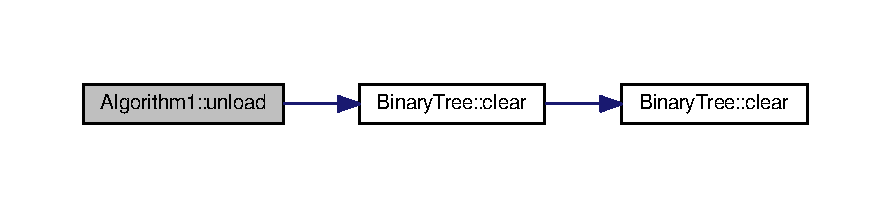
\includegraphics[width=350pt]{class_algorithm1_a135dd26c6c741812d75cd7f2f270592d_cgraph}
\end{center}
\end{figure}




\subsection{Dokumentacja atrybutów składowych}
\hypertarget{class_algorithm1_a3fb7f66d1e4aae77a49c6f7c241f47c9}{\index{Algorithm1@{Algorithm1}!stos@{stos}}
\index{stos@{stos}!Algorithm1@{Algorithm1}}
\subsubsection[{stos}]{\setlength{\rightskip}{0pt plus 5cm}{\bf Stos} Algorithm1\-::stos\hspace{0.3cm}{\ttfamily [private]}}}\label{class_algorithm1_a3fb7f66d1e4aae77a49c6f7c241f47c9}


Definicja w linii 18 pliku algorithm1.\-hh.

\hypertarget{class_algorithm1_a696e1e45bff4a0510dfb76274321583f}{\index{Algorithm1@{Algorithm1}!tab@{tab}}
\index{tab@{tab}!Algorithm1@{Algorithm1}}
\subsubsection[{tab}]{\setlength{\rightskip}{0pt plus 5cm}int$\ast$ Algorithm1\-::tab\hspace{0.3cm}{\ttfamily [private]}}}\label{class_algorithm1_a696e1e45bff4a0510dfb76274321583f}


Definicja w linii 14 pliku algorithm1.\-hh.



Dokumentacja dla tej klasy została wygenerowana z plików\-:\begin{DoxyCompactItemize}
\item 
\hyperlink{algorithm1_8hh}{algorithm1.\-hh}\item 
\hyperlink{algorithm1_8cpp}{algorithm1.\-cpp}\end{DoxyCompactItemize}

\hypertarget{class_algorithm2}{\section{Dokumentacja klasy Algorithm2}
\label{class_algorithm2}\index{Algorithm2@{Algorithm2}}
}


Klasa \hyperlink{class_algorithm2}{Algorithm2} modelujaca algorytm sortowania stosu. Obiekt tego typu reprezentuje algorytm wykonujacy sortowanie szybkie na elementach stosu. Dziedziczy po klasie \hyperlink{class_benchmark}{Benchmark}.  




{\ttfamily \#include $<$algorithm2.\-hh$>$}



Diagram dziedziczenia dla Algorithm2\nopagebreak
\begin{figure}[H]
\begin{center}
\leavevmode
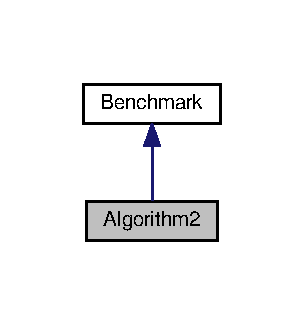
\includegraphics[width=146pt]{class_algorithm2__inherit__graph}
\end{center}
\end{figure}


Diagram współpracy dla Algorithm2\-:\nopagebreak
\begin{figure}[H]
\begin{center}
\leavevmode
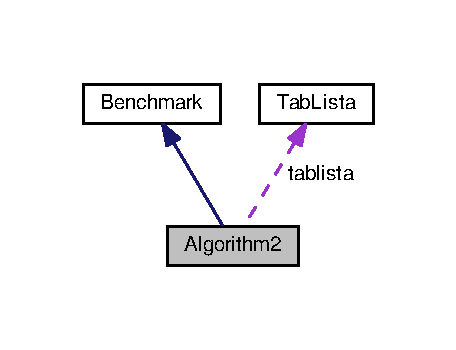
\includegraphics[width=259pt]{class_algorithm2__coll__graph}
\end{center}
\end{figure}
\subsection*{Metody publiczne}
\begin{DoxyCompactItemize}
\item 
\hyperlink{class_algorithm2_ad77a51433815456eca8139444e78b49b}{Algorithm2} ()
\begin{DoxyCompactList}\small\item\em Konstruktor obiektu \hyperlink{class_algorithm2}{Algorithm2}. \end{DoxyCompactList}\item 
\hyperlink{class_algorithm2_a63a761a11070a07905229137034b3cb9}{Algorithm2} (unsigned short $\ast$\-\_\-tab, int \-\_\-id)
\begin{DoxyCompactList}\small\item\em Konstruktor parametryczny obiektu \hyperlink{class_algorithm2}{Algorithm2}. \end{DoxyCompactList}\item 
\hyperlink{class_algorithm2_ab2c630f56f5d2e90f62a13fdaf0cd954}{$\sim$\-Algorithm2} ()
\begin{DoxyCompactList}\small\item\em Destruktor obiektu \hyperlink{class_algorithm2}{Algorithm2}. \end{DoxyCompactList}\item 
virtual void \hyperlink{class_algorithm2_a50bbb4421660c4200dba66e9da9d7969}{load} (int \-\_\-border)
\begin{DoxyCompactList}\small\item\em Metoda przygotowywania algorytmu. Metoda sluzy do przygotowania warunkow do przeprowadzenia testu. \end{DoxyCompactList}\item 
virtual void \hyperlink{class_algorithm2_a3d7e4d0c9308d0b97250cb5596a73165}{unload} (int \-\_\-border)
\begin{DoxyCompactList}\small\item\em Metoda sprzatania. Metoda sluzy do oproznienia struktury. \end{DoxyCompactList}\item 
virtual void \hyperlink{class_algorithm2_a409e58d5fb0b6d2407cc986cf163703b}{run\-Algorithm} (int \-\_\-border)
\begin{DoxyCompactList}\small\item\em Metoda uruchamiania algorytmu. Metoda sluzy do wykonywania danego algorytmu. Sortuje elementy stosu. \end{DoxyCompactList}\end{DoxyCompactItemize}
\subsection*{Atrybuty prywatne}
\begin{DoxyCompactItemize}
\item 
\hyperlink{struct_binary_tree}{Binary\-Tree} \hyperlink{class_algorithm2_aff7c12a2dc0294d120a36ae0efc4af6a}{tree}
\begin{DoxyCompactList}\small\item\em Zmienna przechowujaca drzewo binarne. \end{DoxyCompactList}\end{DoxyCompactItemize}
\subsection*{Dodatkowe Dziedziczone Składowe}


\subsection{Opis szczegółowy}


Definicja w linii 10 pliku algorithm2.\-hh.



\subsection{Dokumentacja konstruktora i destruktora}
\hypertarget{class_algorithm2_ad77a51433815456eca8139444e78b49b}{\index{Algorithm2@{Algorithm2}!Algorithm2@{Algorithm2}}
\index{Algorithm2@{Algorithm2}!Algorithm2@{Algorithm2}}
\subsubsection[{Algorithm2}]{\setlength{\rightskip}{0pt plus 5cm}Algorithm2\-::\-Algorithm2 (
\begin{DoxyParamCaption}
{}
\end{DoxyParamCaption}
)\hspace{0.3cm}{\ttfamily [inline]}}}\label{class_algorithm2_ad77a51433815456eca8139444e78b49b}


Definicja w linii 20 pliku algorithm2.\-hh.

\hypertarget{class_algorithm2_a63a761a11070a07905229137034b3cb9}{\index{Algorithm2@{Algorithm2}!Algorithm2@{Algorithm2}}
\index{Algorithm2@{Algorithm2}!Algorithm2@{Algorithm2}}
\subsubsection[{Algorithm2}]{\setlength{\rightskip}{0pt plus 5cm}Algorithm2\-::\-Algorithm2 (
\begin{DoxyParamCaption}
\item[{unsigned short $\ast$}]{\-\_\-tab, }
\item[{int}]{\-\_\-id}
\end{DoxyParamCaption}
)}}\label{class_algorithm2_a63a761a11070a07905229137034b3cb9}

\begin{DoxyParams}[1]{Parametry}
\mbox{\tt in}  & {\em \-\_\-tab} & -\/ tablica przechowujaca dane wejsciowe. \\
\hline
\mbox{\tt in}  & {\em \-\_\-id} & -\/ identyfikator algorytmu. \\
\hline
\end{DoxyParams}


Definicja w linii 10 pliku algorithm2.\-cpp.

\hypertarget{class_algorithm2_ab2c630f56f5d2e90f62a13fdaf0cd954}{\index{Algorithm2@{Algorithm2}!$\sim$\-Algorithm2@{$\sim$\-Algorithm2}}
\index{$\sim$\-Algorithm2@{$\sim$\-Algorithm2}!Algorithm2@{Algorithm2}}
\subsubsection[{$\sim$\-Algorithm2}]{\setlength{\rightskip}{0pt plus 5cm}Algorithm2\-::$\sim$\-Algorithm2 (
\begin{DoxyParamCaption}
{}
\end{DoxyParamCaption}
)}}\label{class_algorithm2_ab2c630f56f5d2e90f62a13fdaf0cd954}


Definicja w linii 17 pliku algorithm2.\-cpp.



\subsection{Dokumentacja funkcji składowych}
\hypertarget{class_algorithm2_a50bbb4421660c4200dba66e9da9d7969}{\index{Algorithm2@{Algorithm2}!load@{load}}
\index{load@{load}!Algorithm2@{Algorithm2}}
\subsubsection[{load}]{\setlength{\rightskip}{0pt plus 5cm}void Algorithm2\-::load (
\begin{DoxyParamCaption}
\item[{int}]{\-\_\-border}
\end{DoxyParamCaption}
)\hspace{0.3cm}{\ttfamily [virtual]}}}\label{class_algorithm2_a50bbb4421660c4200dba66e9da9d7969}

\begin{DoxyParams}[1]{Parametry}
\mbox{\tt in}  & {\em \-\_\-border} & -\/ ilosc elementow dla ktorych metoda ma wykonac swoje dzialanie. \\
\hline
\end{DoxyParams}


Implementuje \hyperlink{class_benchmark_a41f66d36949f1488facb8e3d49c99f67}{Benchmark}.



Definicja w linii 28 pliku algorithm2.\-cpp.



Oto graf wywołań dla tej funkcji\-:\nopagebreak
\begin{figure}[H]
\begin{center}
\leavevmode
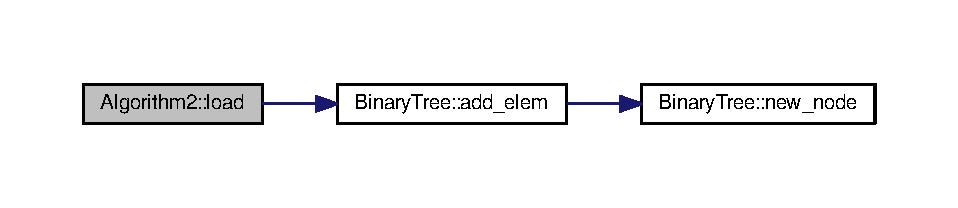
\includegraphics[width=350pt]{class_algorithm2_a50bbb4421660c4200dba66e9da9d7969_cgraph}
\end{center}
\end{figure}


\hypertarget{class_algorithm2_a409e58d5fb0b6d2407cc986cf163703b}{\index{Algorithm2@{Algorithm2}!run\-Algorithm@{run\-Algorithm}}
\index{run\-Algorithm@{run\-Algorithm}!Algorithm2@{Algorithm2}}
\subsubsection[{run\-Algorithm}]{\setlength{\rightskip}{0pt plus 5cm}void Algorithm2\-::run\-Algorithm (
\begin{DoxyParamCaption}
\item[{int}]{\-\_\-border}
\end{DoxyParamCaption}
)\hspace{0.3cm}{\ttfamily [virtual]}}}\label{class_algorithm2_a409e58d5fb0b6d2407cc986cf163703b}

\begin{DoxyParams}[1]{Parametry}
\mbox{\tt in}  & {\em \-\_\-border} & -\/ ilosc elementow dla ktorych algorytm ma wykonac swoje dzialanie. \\
\hline
\end{DoxyParams}


Implementuje \hyperlink{class_benchmark_a33e60395b1e126ca65c3aea3abf6debf}{Benchmark}.



Definicja w linii 22 pliku algorithm2.\-cpp.



Oto graf wywołań dla tej funkcji\-:\nopagebreak
\begin{figure}[H]
\begin{center}
\leavevmode
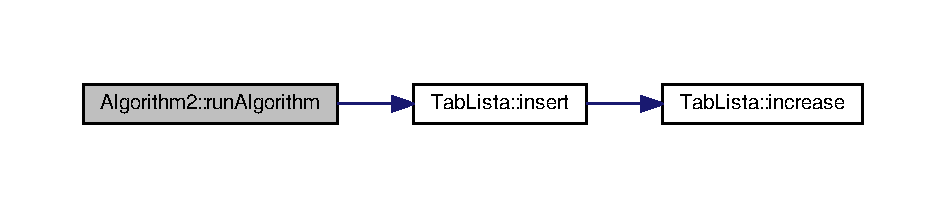
\includegraphics[width=350pt]{class_algorithm2_a409e58d5fb0b6d2407cc986cf163703b_cgraph}
\end{center}
\end{figure}


\hypertarget{class_algorithm2_a3d7e4d0c9308d0b97250cb5596a73165}{\index{Algorithm2@{Algorithm2}!unload@{unload}}
\index{unload@{unload}!Algorithm2@{Algorithm2}}
\subsubsection[{unload}]{\setlength{\rightskip}{0pt plus 5cm}void Algorithm2\-::unload (
\begin{DoxyParamCaption}
\item[{int}]{\-\_\-border}
\end{DoxyParamCaption}
)\hspace{0.3cm}{\ttfamily [virtual]}}}\label{class_algorithm2_a3d7e4d0c9308d0b97250cb5596a73165}

\begin{DoxyParams}[1]{Parametry}
\mbox{\tt in}  & {\em \-\_\-border} & -\/ ilosc elementow dla ktorych metoda ma wykonac swoje dzialanie. \\
\hline
\end{DoxyParams}


Implementuje \hyperlink{class_benchmark_a2dcfb6ee9e648ae88d8c131b2b191bed}{Benchmark}.



Definicja w linii 35 pliku algorithm2.\-cpp.



Oto graf wywołań dla tej funkcji\-:\nopagebreak
\begin{figure}[H]
\begin{center}
\leavevmode
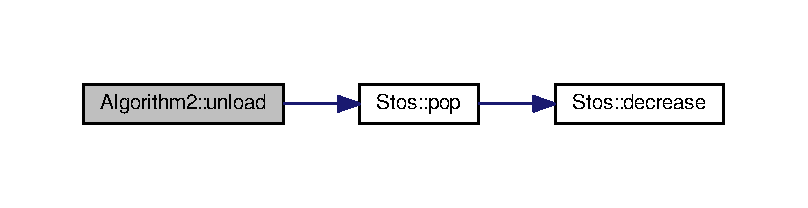
\includegraphics[width=350pt]{class_algorithm2_a3d7e4d0c9308d0b97250cb5596a73165_cgraph}
\end{center}
\end{figure}




\subsection{Dokumentacja atrybutów składowych}
\hypertarget{class_algorithm2_aff7c12a2dc0294d120a36ae0efc4af6a}{\index{Algorithm2@{Algorithm2}!tree@{tree}}
\index{tree@{tree}!Algorithm2@{Algorithm2}}
\subsubsection[{tree}]{\setlength{\rightskip}{0pt plus 5cm}{\bf Binary\-Tree} Algorithm2\-::tree\hspace{0.3cm}{\ttfamily [private]}}}\label{class_algorithm2_aff7c12a2dc0294d120a36ae0efc4af6a}


Definicja w linii 14 pliku algorithm2.\-hh.



Dokumentacja dla tej klasy została wygenerowana z plików\-:\begin{DoxyCompactItemize}
\item 
\hyperlink{algorithm2_8hh}{algorithm2.\-hh}\item 
\hyperlink{algorithm2_8cpp}{algorithm2.\-cpp}\end{DoxyCompactItemize}

\hypertarget{class_algorithm3}{\section{Dokumentacja klasy Algorithm3}
\label{class_algorithm3}\index{Algorithm3@{Algorithm3}}
}


Klasa \hyperlink{class_algorithm3}{Algorithm3} modelujaca algorytm sortowania stosu. Obiekt tego typu reprezentuje algorytm wykonujacy sortowanie szybkie na elementach stosu. Dziedziczy po klasie \hyperlink{class_benchmark}{Benchmark}.  




{\ttfamily \#include $<$algorithm3.\-hh$>$}



Diagram dziedziczenia dla Algorithm3
\nopagebreak
\begin{figure}[H]
\begin{center}
\leavevmode
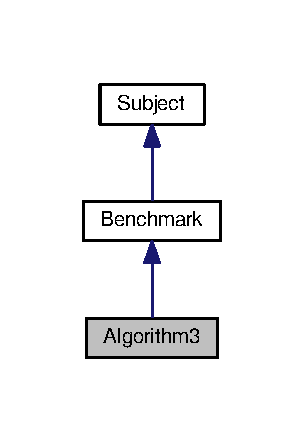
\includegraphics[width=146pt]{class_algorithm3__inherit__graph}
\end{center}
\end{figure}


Diagram współpracy dla Algorithm3\-:
\nopagebreak
\begin{figure}[H]
\begin{center}
\leavevmode
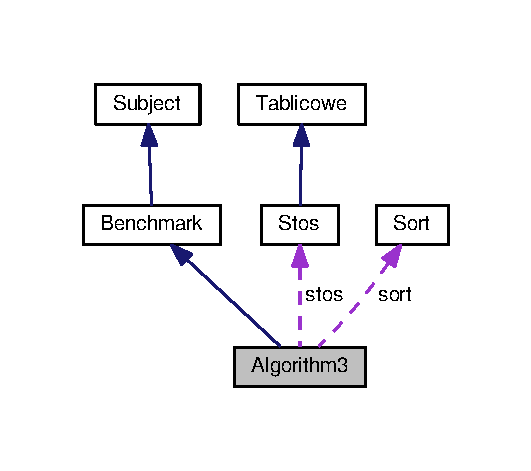
\includegraphics[width=255pt]{class_algorithm3__coll__graph}
\end{center}
\end{figure}
\subsection*{Metody publiczne}
\begin{DoxyCompactItemize}
\item 
\hyperlink{class_algorithm3_a88d9f8567616fd898bf202602726600d}{Algorithm3} ()
\begin{DoxyCompactList}\small\item\em Konstruktor obiektu \hyperlink{class_algorithm3}{Algorithm3}. \end{DoxyCompactList}\item 
\hyperlink{class_algorithm3_a71f0a79b028ae3c867321bcf19a45188}{Algorithm3} (unsigned short $\ast$\-\_\-tab, int \-\_\-id)
\begin{DoxyCompactList}\small\item\em Konstruktor parametryczny obiektu \hyperlink{class_algorithm3}{Algorithm3}. \end{DoxyCompactList}\item 
\hyperlink{class_algorithm3_ae9d1f5425fce3fc93d356fe8bf103e28}{$\sim$\-Algorithm3} ()
\begin{DoxyCompactList}\small\item\em Destruktor obiektu \hyperlink{class_algorithm3}{Algorithm3}. \end{DoxyCompactList}\item 
virtual void \hyperlink{class_algorithm3_a92b082327e99863c82981cdaec9a45a1}{load} (int \-\_\-border)
\begin{DoxyCompactList}\small\item\em Metoda przygotowywania algorytmu. Metoda sluzy do przygotowania warunkow do przeprowadzenia testu. \end{DoxyCompactList}\item 
virtual void \hyperlink{class_algorithm3_a170d77ee28866741214e65da7efcf533}{unload} (int \-\_\-border)
\begin{DoxyCompactList}\small\item\em Metoda sprzatania. Metoda sluzy do oproznienia struktury. \end{DoxyCompactList}\item 
virtual void \hyperlink{class_algorithm3_ac5c80b248190a12fa770e0386f694570}{run\-Algorithm} (int \-\_\-border)
\begin{DoxyCompactList}\small\item\em Metoda uruchamiania algorytmu. Metoda sluzy do wykonywania danego algorytmu. Sortuje elementy stosu. \end{DoxyCompactList}\end{DoxyCompactItemize}
\subsection*{Atrybuty prywatne}
\begin{DoxyCompactItemize}
\item 
\hyperlink{class_r_b_tree}{R\-B\-Tree} \hyperlink{class_algorithm3_a258233c4774afd7d6e6d5a1198955556}{tree}
\begin{DoxyCompactList}\small\item\em Zmienna przechowujaca drzewo czerwono-\/czarne. \end{DoxyCompactList}\end{DoxyCompactItemize}
\subsection*{Dodatkowe Dziedziczone Składowe}


\subsection{Opis szczegółowy}


Definicja w linii 10 pliku algorithm3.\-hh.



\subsection{Dokumentacja konstruktora i destruktora}
\hypertarget{class_algorithm3_a88d9f8567616fd898bf202602726600d}{\index{Algorithm3@{Algorithm3}!Algorithm3@{Algorithm3}}
\index{Algorithm3@{Algorithm3}!Algorithm3@{Algorithm3}}
\subsubsection[{Algorithm3}]{\setlength{\rightskip}{0pt plus 5cm}Algorithm3\-::\-Algorithm3 (
\begin{DoxyParamCaption}
{}
\end{DoxyParamCaption}
)\hspace{0.3cm}{\ttfamily [inline]}}}\label{class_algorithm3_a88d9f8567616fd898bf202602726600d}


Definicja w linii 20 pliku algorithm3.\-hh.

\hypertarget{class_algorithm3_a71f0a79b028ae3c867321bcf19a45188}{\index{Algorithm3@{Algorithm3}!Algorithm3@{Algorithm3}}
\index{Algorithm3@{Algorithm3}!Algorithm3@{Algorithm3}}
\subsubsection[{Algorithm3}]{\setlength{\rightskip}{0pt plus 5cm}Algorithm3\-::\-Algorithm3 (
\begin{DoxyParamCaption}
\item[{unsigned short $\ast$}]{\-\_\-tab, }
\item[{int}]{\-\_\-id}
\end{DoxyParamCaption}
)}}\label{class_algorithm3_a71f0a79b028ae3c867321bcf19a45188}

\begin{DoxyParams}[1]{Parametry}
\mbox{\tt in}  & {\em \-\_\-tab} & -\/ tablica przechowujaca dane wejsciowe. \\
\hline
\mbox{\tt in}  & {\em \-\_\-id} & -\/ identyfikator algorytmu. \\
\hline
\end{DoxyParams}


Definicja w linii 10 pliku algorithm3.\-cpp.

\hypertarget{class_algorithm3_ae9d1f5425fce3fc93d356fe8bf103e28}{\index{Algorithm3@{Algorithm3}!$\sim$\-Algorithm3@{$\sim$\-Algorithm3}}
\index{$\sim$\-Algorithm3@{$\sim$\-Algorithm3}!Algorithm3@{Algorithm3}}
\subsubsection[{$\sim$\-Algorithm3}]{\setlength{\rightskip}{0pt plus 5cm}Algorithm3\-::$\sim$\-Algorithm3 (
\begin{DoxyParamCaption}
{}
\end{DoxyParamCaption}
)}}\label{class_algorithm3_ae9d1f5425fce3fc93d356fe8bf103e28}


Definicja w linii 17 pliku algorithm3.\-cpp.



\subsection{Dokumentacja funkcji składowych}
\hypertarget{class_algorithm3_a92b082327e99863c82981cdaec9a45a1}{\index{Algorithm3@{Algorithm3}!load@{load}}
\index{load@{load}!Algorithm3@{Algorithm3}}
\subsubsection[{load}]{\setlength{\rightskip}{0pt plus 5cm}void Algorithm3\-::load (
\begin{DoxyParamCaption}
\item[{int}]{\-\_\-border}
\end{DoxyParamCaption}
)\hspace{0.3cm}{\ttfamily [virtual]}}}\label{class_algorithm3_a92b082327e99863c82981cdaec9a45a1}

\begin{DoxyParams}[1]{Parametry}
\mbox{\tt in}  & {\em \-\_\-border} & -\/ ilosc elementow dla ktorych metoda ma wykonac swoje dzialanie. \\
\hline
\end{DoxyParams}


Implementuje \hyperlink{class_benchmark_a41f66d36949f1488facb8e3d49c99f67}{Benchmark}.



Definicja w linii 29 pliku algorithm3.\-cpp.

\hypertarget{class_algorithm3_ac5c80b248190a12fa770e0386f694570}{\index{Algorithm3@{Algorithm3}!run\-Algorithm@{run\-Algorithm}}
\index{run\-Algorithm@{run\-Algorithm}!Algorithm3@{Algorithm3}}
\subsubsection[{run\-Algorithm}]{\setlength{\rightskip}{0pt plus 5cm}void Algorithm3\-::run\-Algorithm (
\begin{DoxyParamCaption}
\item[{int}]{\-\_\-border}
\end{DoxyParamCaption}
)\hspace{0.3cm}{\ttfamily [virtual]}}}\label{class_algorithm3_ac5c80b248190a12fa770e0386f694570}

\begin{DoxyParams}[1]{Parametry}
\mbox{\tt in}  & {\em \-\_\-border} & -\/ ilosc elementow dla ktorych algorytm ma wykonac swoje dzialanie. \\
\hline
\end{DoxyParams}


Implementuje \hyperlink{class_benchmark_a33e60395b1e126ca65c3aea3abf6debf}{Benchmark}.



Definicja w linii 22 pliku algorithm3.\-cpp.



Oto graf wywołań dla tej funkcji\-:
\nopagebreak
\begin{figure}[H]
\begin{center}
\leavevmode
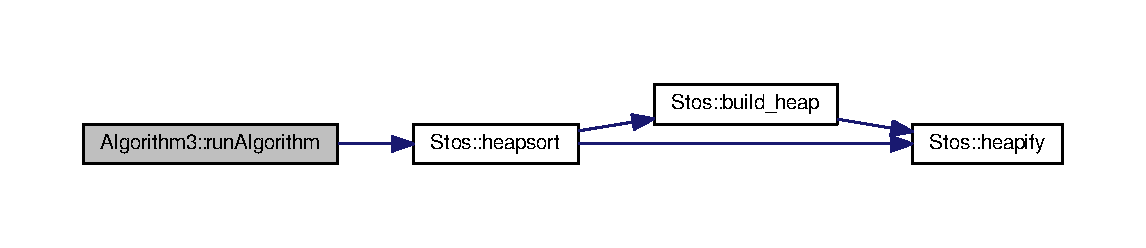
\includegraphics[width=350pt]{class_algorithm3_ac5c80b248190a12fa770e0386f694570_cgraph}
\end{center}
\end{figure}


\hypertarget{class_algorithm3_a170d77ee28866741214e65da7efcf533}{\index{Algorithm3@{Algorithm3}!unload@{unload}}
\index{unload@{unload}!Algorithm3@{Algorithm3}}
\subsubsection[{unload}]{\setlength{\rightskip}{0pt plus 5cm}void Algorithm3\-::unload (
\begin{DoxyParamCaption}
\item[{int}]{\-\_\-border}
\end{DoxyParamCaption}
)\hspace{0.3cm}{\ttfamily [virtual]}}}\label{class_algorithm3_a170d77ee28866741214e65da7efcf533}

\begin{DoxyParams}[1]{Parametry}
\mbox{\tt in}  & {\em \-\_\-border} & -\/ ilosc elementow dla ktorych metoda ma wykonac swoje dzialanie. \\
\hline
\end{DoxyParams}


Implementuje \hyperlink{class_benchmark_a2dcfb6ee9e648ae88d8c131b2b191bed}{Benchmark}.



Definicja w linii 34 pliku algorithm3.\-cpp.



Oto graf wywołań dla tej funkcji\-:
\nopagebreak
\begin{figure}[H]
\begin{center}
\leavevmode
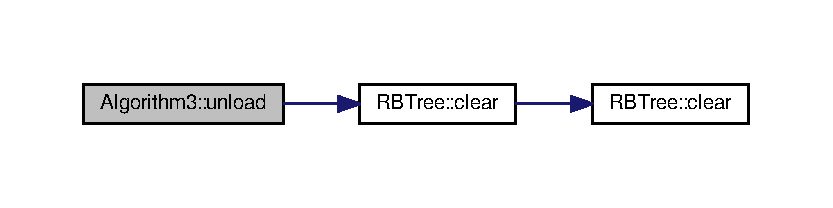
\includegraphics[width=350pt]{class_algorithm3_a170d77ee28866741214e65da7efcf533_cgraph}
\end{center}
\end{figure}




\subsection{Dokumentacja atrybutów składowych}
\hypertarget{class_algorithm3_a258233c4774afd7d6e6d5a1198955556}{\index{Algorithm3@{Algorithm3}!tree@{tree}}
\index{tree@{tree}!Algorithm3@{Algorithm3}}
\subsubsection[{tree}]{\setlength{\rightskip}{0pt plus 5cm}{\bf R\-B\-Tree} Algorithm3\-::tree\hspace{0.3cm}{\ttfamily [private]}}}\label{class_algorithm3_a258233c4774afd7d6e6d5a1198955556}


Definicja w linii 14 pliku algorithm3.\-hh.



Dokumentacja dla tej klasy została wygenerowana z plików\-:\begin{DoxyCompactItemize}
\item 
\hyperlink{algorithm3_8hh}{algorithm3.\-hh}\item 
\hyperlink{algorithm3_8cpp}{algorithm3.\-cpp}\end{DoxyCompactItemize}

\hypertarget{class_algorithm4}{\section{Dokumentacja klasy Algorithm4}
\label{class_algorithm4}\index{Algorithm4@{Algorithm4}}
}


Klasa \hyperlink{class_algorithm4}{Algorithm4} modelujaca algorytm sortowania stosu. Obiekt tego typu reprezentuje algorytm wykonujacy sortowanie szybkie po optymalizacji na elementach stosu. Dziedziczy po klasie \hyperlink{class_benchmark}{Benchmark}.  




{\ttfamily \#include $<$algorithm4.\-hh$>$}



Diagram dziedziczenia dla Algorithm4\nopagebreak
\begin{figure}[H]
\begin{center}
\leavevmode
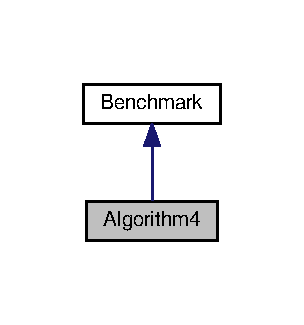
\includegraphics[width=146pt]{class_algorithm4__inherit__graph}
\end{center}
\end{figure}


Diagram współpracy dla Algorithm4\-:\nopagebreak
\begin{figure}[H]
\begin{center}
\leavevmode
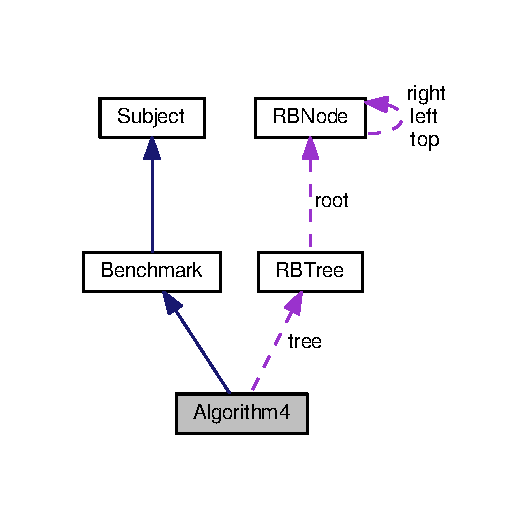
\includegraphics[width=255pt]{class_algorithm4__coll__graph}
\end{center}
\end{figure}
\subsection*{Metody publiczne}
\begin{DoxyCompactItemize}
\item 
\hyperlink{class_algorithm4_a79f0bdede29ae14437031022b7a32278}{Algorithm4} ()
\begin{DoxyCompactList}\small\item\em Konstruktor obiektu \hyperlink{class_algorithm4}{Algorithm4}. \end{DoxyCompactList}\item 
\hyperlink{class_algorithm4_a7e9812499c980dfc9e2032d1a3728b09}{Algorithm4} (unsigned short $\ast$\-\_\-tab, int \-\_\-id)
\begin{DoxyCompactList}\small\item\em Konstruktor parametryczny obiektu \hyperlink{class_algorithm4}{Algorithm4}. \end{DoxyCompactList}\item 
\hyperlink{class_algorithm4_ad73b6bd1ca2b289db737e3e4f5b40abf}{$\sim$\-Algorithm4} ()
\begin{DoxyCompactList}\small\item\em Destruktor obiektu \hyperlink{class_algorithm4}{Algorithm4}. \end{DoxyCompactList}\item 
virtual void \hyperlink{class_algorithm4_aa86adbf6be3052692f885c1be28b2300}{load} (int \-\_\-border)
\begin{DoxyCompactList}\small\item\em Metoda przygotowywania algorytmu. Metoda sluzy do przygotowania warunkow do przeprowadzenia testu. \end{DoxyCompactList}\item 
virtual void \hyperlink{class_algorithm4_a673e2d2373378ab01a7f0378d978f162}{unload} (int \-\_\-border)
\begin{DoxyCompactList}\small\item\em Metoda sprzatania. Metoda sluzy do oproznienia struktury. \end{DoxyCompactList}\item 
virtual void \hyperlink{class_algorithm4_ad1e715e2d6ddec7607f3cafa77443cd2}{run\-Algorithm} (int \-\_\-border)
\begin{DoxyCompactList}\small\item\em Metoda uruchamiania algorytmu. Metoda sluzy do wykonywania danego algorytmu. Sortuje elementy stosu. \end{DoxyCompactList}\end{DoxyCompactItemize}
\subsection*{Atrybuty prywatne}
\begin{DoxyCompactItemize}
\item 
\hyperlink{struct_stos}{Stos} \hyperlink{class_algorithm4_aa9946110dc906caed6ddc49c60f7a3c8}{stos}
\begin{DoxyCompactList}\small\item\em Zmienna przechowujaca stos. \end{DoxyCompactList}\item 
\hyperlink{class_sort}{Sort} \hyperlink{class_algorithm4_afbc43ff18fc5837d95e5746353bfc54a}{sort}
\begin{DoxyCompactList}\small\item\em Zmienna przechowujaca klase sortujaca. \end{DoxyCompactList}\end{DoxyCompactItemize}
\subsection*{Dodatkowe Dziedziczone Składowe}


\subsection{Opis szczegółowy}


Definicja w linii 10 pliku algorithm4.\-hh.



\subsection{Dokumentacja konstruktora i destruktora}
\hypertarget{class_algorithm4_a79f0bdede29ae14437031022b7a32278}{\index{Algorithm4@{Algorithm4}!Algorithm4@{Algorithm4}}
\index{Algorithm4@{Algorithm4}!Algorithm4@{Algorithm4}}
\subsubsection[{Algorithm4}]{\setlength{\rightskip}{0pt plus 5cm}Algorithm4\-::\-Algorithm4 (
\begin{DoxyParamCaption}
{}
\end{DoxyParamCaption}
)\hspace{0.3cm}{\ttfamily [inline]}}}\label{class_algorithm4_a79f0bdede29ae14437031022b7a32278}


Definicja w linii 24 pliku algorithm4.\-hh.

\hypertarget{class_algorithm4_a7e9812499c980dfc9e2032d1a3728b09}{\index{Algorithm4@{Algorithm4}!Algorithm4@{Algorithm4}}
\index{Algorithm4@{Algorithm4}!Algorithm4@{Algorithm4}}
\subsubsection[{Algorithm4}]{\setlength{\rightskip}{0pt plus 5cm}Algorithm4\-::\-Algorithm4 (
\begin{DoxyParamCaption}
\item[{unsigned short $\ast$}]{\-\_\-tab, }
\item[{int}]{\-\_\-id}
\end{DoxyParamCaption}
)}}\label{class_algorithm4_a7e9812499c980dfc9e2032d1a3728b09}

\begin{DoxyParams}[1]{Parametry}
\mbox{\tt in}  & {\em \-\_\-tab} & -\/ tablica przechowujaca dane wejsciowe. \\
\hline
\mbox{\tt in}  & {\em \-\_\-id} & -\/ identyfikator algorytmu. \\
\hline
\end{DoxyParams}


Definicja w linii 12 pliku algorithm4.\-cpp.

\hypertarget{class_algorithm4_ad73b6bd1ca2b289db737e3e4f5b40abf}{\index{Algorithm4@{Algorithm4}!$\sim$\-Algorithm4@{$\sim$\-Algorithm4}}
\index{$\sim$\-Algorithm4@{$\sim$\-Algorithm4}!Algorithm4@{Algorithm4}}
\subsubsection[{$\sim$\-Algorithm4}]{\setlength{\rightskip}{0pt plus 5cm}Algorithm4\-::$\sim$\-Algorithm4 (
\begin{DoxyParamCaption}
{}
\end{DoxyParamCaption}
)}}\label{class_algorithm4_ad73b6bd1ca2b289db737e3e4f5b40abf}


Definicja w linii 19 pliku algorithm4.\-cpp.



\subsection{Dokumentacja funkcji składowych}
\hypertarget{class_algorithm4_aa86adbf6be3052692f885c1be28b2300}{\index{Algorithm4@{Algorithm4}!load@{load}}
\index{load@{load}!Algorithm4@{Algorithm4}}
\subsubsection[{load}]{\setlength{\rightskip}{0pt plus 5cm}void Algorithm4\-::load (
\begin{DoxyParamCaption}
\item[{int}]{\-\_\-border}
\end{DoxyParamCaption}
)\hspace{0.3cm}{\ttfamily [virtual]}}}\label{class_algorithm4_aa86adbf6be3052692f885c1be28b2300}

\begin{DoxyParams}[1]{Parametry}
\mbox{\tt in}  & {\em \-\_\-border} & -\/ ilosc elementow dla ktorych metoda ma wykonac swoje dzialanie. \\
\hline
\end{DoxyParams}


Implementuje \hyperlink{class_benchmark_a41f66d36949f1488facb8e3d49c99f67}{Benchmark}.



Definicja w linii 30 pliku algorithm4.\-cpp.



Oto graf wywołań dla tej funkcji\-:\nopagebreak
\begin{figure}[H]
\begin{center}
\leavevmode
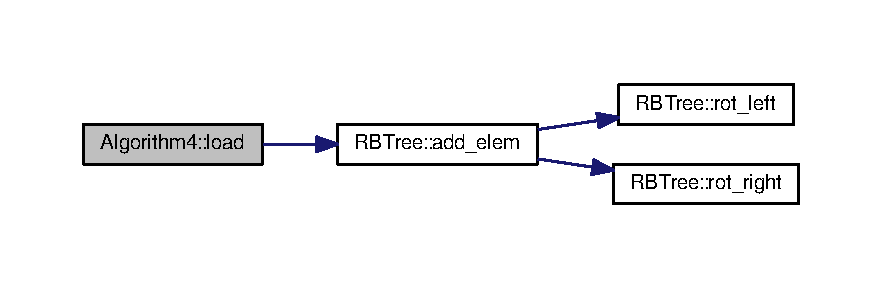
\includegraphics[width=350pt]{class_algorithm4_aa86adbf6be3052692f885c1be28b2300_cgraph}
\end{center}
\end{figure}


\hypertarget{class_algorithm4_ad1e715e2d6ddec7607f3cafa77443cd2}{\index{Algorithm4@{Algorithm4}!run\-Algorithm@{run\-Algorithm}}
\index{run\-Algorithm@{run\-Algorithm}!Algorithm4@{Algorithm4}}
\subsubsection[{run\-Algorithm}]{\setlength{\rightskip}{0pt plus 5cm}void Algorithm4\-::run\-Algorithm (
\begin{DoxyParamCaption}
\item[{int}]{\-\_\-border}
\end{DoxyParamCaption}
)\hspace{0.3cm}{\ttfamily [virtual]}}}\label{class_algorithm4_ad1e715e2d6ddec7607f3cafa77443cd2}

\begin{DoxyParams}[1]{Parametry}
\mbox{\tt in}  & {\em \-\_\-border} & -\/ ilosc elementow dla ktorych algorytm ma wykonac swoje dzialanie. \\
\hline
\end{DoxyParams}


Implementuje \hyperlink{class_benchmark_a33e60395b1e126ca65c3aea3abf6debf}{Benchmark}.



Definicja w linii 24 pliku algorithm4.\-cpp.



Oto graf wywołań dla tej funkcji\-:\nopagebreak
\begin{figure}[H]
\begin{center}
\leavevmode
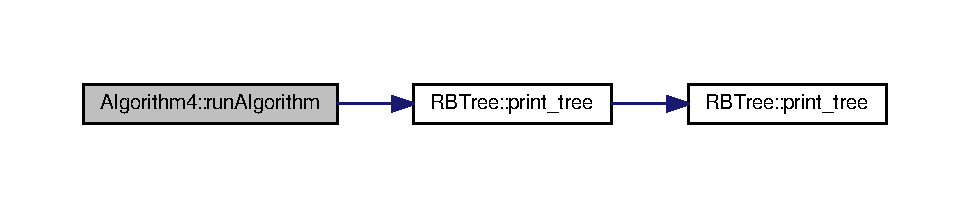
\includegraphics[width=322pt]{class_algorithm4_ad1e715e2d6ddec7607f3cafa77443cd2_cgraph}
\end{center}
\end{figure}


\hypertarget{class_algorithm4_a673e2d2373378ab01a7f0378d978f162}{\index{Algorithm4@{Algorithm4}!unload@{unload}}
\index{unload@{unload}!Algorithm4@{Algorithm4}}
\subsubsection[{unload}]{\setlength{\rightskip}{0pt plus 5cm}void Algorithm4\-::unload (
\begin{DoxyParamCaption}
\item[{int}]{\-\_\-border}
\end{DoxyParamCaption}
)\hspace{0.3cm}{\ttfamily [virtual]}}}\label{class_algorithm4_a673e2d2373378ab01a7f0378d978f162}

\begin{DoxyParams}[1]{Parametry}
\mbox{\tt in}  & {\em \-\_\-border} & -\/ ilosc elementow dla ktorych metoda ma wykonac swoje dzialanie. \\
\hline
\end{DoxyParams}


Implementuje \hyperlink{class_benchmark_a2dcfb6ee9e648ae88d8c131b2b191bed}{Benchmark}.



Definicja w linii 36 pliku algorithm4.\-cpp.



Oto graf wywołań dla tej funkcji\-:\nopagebreak
\begin{figure}[H]
\begin{center}
\leavevmode
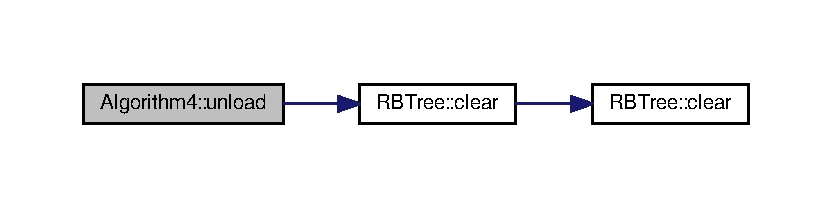
\includegraphics[width=350pt]{class_algorithm4_a673e2d2373378ab01a7f0378d978f162_cgraph}
\end{center}
\end{figure}




\subsection{Dokumentacja atrybutów składowych}
\hypertarget{class_algorithm4_afbc43ff18fc5837d95e5746353bfc54a}{\index{Algorithm4@{Algorithm4}!sort@{sort}}
\index{sort@{sort}!Algorithm4@{Algorithm4}}
\subsubsection[{sort}]{\setlength{\rightskip}{0pt plus 5cm}{\bf Sort} Algorithm4\-::sort\hspace{0.3cm}{\ttfamily [private]}}}\label{class_algorithm4_afbc43ff18fc5837d95e5746353bfc54a}


Definicja w linii 18 pliku algorithm4.\-hh.

\hypertarget{class_algorithm4_aa9946110dc906caed6ddc49c60f7a3c8}{\index{Algorithm4@{Algorithm4}!stos@{stos}}
\index{stos@{stos}!Algorithm4@{Algorithm4}}
\subsubsection[{stos}]{\setlength{\rightskip}{0pt plus 5cm}{\bf Stos} Algorithm4\-::stos\hspace{0.3cm}{\ttfamily [private]}}}\label{class_algorithm4_aa9946110dc906caed6ddc49c60f7a3c8}


Definicja w linii 14 pliku algorithm4.\-hh.



Dokumentacja dla tej klasy została wygenerowana z plików\-:\begin{DoxyCompactItemize}
\item 
\hyperlink{algorithm4_8hh}{algorithm4.\-hh}\item 
\hyperlink{algorithm4_8cpp}{algorithm4.\-cpp}\end{DoxyCompactItemize}

\hypertarget{struct_a_node}{\section{Dokumentacja struktury A\-Node}
\label{struct_a_node}\index{A\-Node@{A\-Node}}
}


Struktura \hyperlink{struct_a_node}{A\-Node}. Obiekt tego typu reprezentuje pojedyncza komorke wraz ze wskaznikiem na nastepna komorke listy.  




{\ttfamily \#include $<$asocjacyjna.\-hh$>$}



Diagram współpracy dla A\-Node\-:
\nopagebreak
\begin{figure}[H]
\begin{center}
\leavevmode
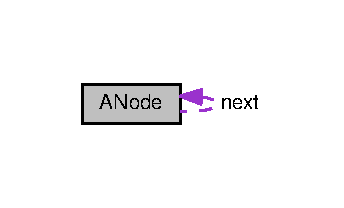
\includegraphics[width=165pt]{struct_a_node__coll__graph}
\end{center}
\end{figure}
\subsection*{Metody publiczne}
\begin{DoxyCompactItemize}
\item 
\hyperlink{struct_a_node_ad12f3f4440ad56e7e90d5ac927ba096a}{A\-Node} (const char $\ast$\-\_\-k)
\begin{DoxyCompactList}\small\item\em Konstruktor paramteryczny struktury \hyperlink{struct_a_node}{A\-Node}. \end{DoxyCompactList}\item 
\hyperlink{struct_a_node_a8fd9487184ba1af2150456919869cd60}{A\-Node} (const \hyperlink{struct_a_node}{A\-Node} \&\-\_\-s)
\begin{DoxyCompactList}\small\item\em Konstruktor paramteryczny struktury \hyperlink{struct_a_node}{A\-Node}. \end{DoxyCompactList}\item 
\hyperlink{struct_a_node_aec880ec60e95396aba5ffdc6ce0a4e8d}{$\sim$\-A\-Node} ()
\begin{DoxyCompactList}\small\item\em Destruktor struktury node. \end{DoxyCompactList}\end{DoxyCompactItemize}
\subsection*{Atrybuty publiczne}
\begin{DoxyCompactItemize}
\item 
\hyperlink{struct_a_node}{A\-Node} $\ast$ \hyperlink{struct_a_node_a97878d7354cd6beff5963e4fd0799805}{next}
\begin{DoxyCompactList}\small\item\em Wskaznik na nastepna komorke. \end{DoxyCompactList}\item 
char $\ast$ \hyperlink{struct_a_node_a3601f1eb35c094a209e3eab174f4afd4}{key}
\begin{DoxyCompactList}\small\item\em Wskaznik na klucz. \end{DoxyCompactList}\item 
int \hyperlink{struct_a_node_a4dbd8d8f9c7082fef7bc7f9113163301}{val}
\begin{DoxyCompactList}\small\item\em Wartosc klucza. \end{DoxyCompactList}\end{DoxyCompactItemize}
\subsection*{Metody prywatne}
\begin{DoxyCompactItemize}
\item 
\hyperlink{struct_a_node}{A\-Node} \& \hyperlink{struct_a_node_a96160014f2ca78c2b7baf21051752dbc}{operator=} (const \hyperlink{struct_a_node}{A\-Node} \&)
\begin{DoxyCompactList}\small\item\em Przeladowanie operatora przypisania. Zabezpieczenie przed automatycznym operatorem przypisania. \end{DoxyCompactList}\end{DoxyCompactItemize}


\subsection{Opis szczegółowy}


Definicja w linii 11 pliku asocjacyjna.\-hh.



\subsection{Dokumentacja konstruktora i destruktora}
\hypertarget{struct_a_node_ad12f3f4440ad56e7e90d5ac927ba096a}{\index{A\-Node@{A\-Node}!A\-Node@{A\-Node}}
\index{A\-Node@{A\-Node}!ANode@{A\-Node}}
\subsubsection[{A\-Node}]{\setlength{\rightskip}{0pt plus 5cm}A\-Node\-::\-A\-Node (
\begin{DoxyParamCaption}
\item[{const char $\ast$}]{\-\_\-k}
\end{DoxyParamCaption}
)}}\label{struct_a_node_ad12f3f4440ad56e7e90d5ac927ba096a}

\begin{DoxyParams}[1]{Parametry}
\mbox{\tt in}  & {\em \-\_\-k} & -\/ wskaznik na klucz. \\
\hline
\end{DoxyParams}


Definicja w linii 8 pliku asocjacyjna.\-cpp.

\hypertarget{struct_a_node_a8fd9487184ba1af2150456919869cd60}{\index{A\-Node@{A\-Node}!A\-Node@{A\-Node}}
\index{A\-Node@{A\-Node}!ANode@{A\-Node}}
\subsubsection[{A\-Node}]{\setlength{\rightskip}{0pt plus 5cm}A\-Node\-::\-A\-Node (
\begin{DoxyParamCaption}
\item[{const {\bf A\-Node} \&}]{\-\_\-s}
\end{DoxyParamCaption}
)}}\label{struct_a_node_a8fd9487184ba1af2150456919869cd60}

\begin{DoxyParams}[1]{Parametry}
\mbox{\tt in}  & {\em \-\_\-s} & -\/ referencja do pary klucz-\/wartosc. \\
\hline
\end{DoxyParams}


Definicja w linii 15 pliku asocjacyjna.\-cpp.

\hypertarget{struct_a_node_aec880ec60e95396aba5ffdc6ce0a4e8d}{\index{A\-Node@{A\-Node}!$\sim$\-A\-Node@{$\sim$\-A\-Node}}
\index{$\sim$\-A\-Node@{$\sim$\-A\-Node}!ANode@{A\-Node}}
\subsubsection[{$\sim$\-A\-Node}]{\setlength{\rightskip}{0pt plus 5cm}A\-Node\-::$\sim$\-A\-Node (
\begin{DoxyParamCaption}
{}
\end{DoxyParamCaption}
)}}\label{struct_a_node_aec880ec60e95396aba5ffdc6ce0a4e8d}


Definicja w linii 29 pliku asocjacyjna.\-cpp.



\subsection{Dokumentacja funkcji składowych}
\hypertarget{struct_a_node_a96160014f2ca78c2b7baf21051752dbc}{\index{A\-Node@{A\-Node}!operator=@{operator=}}
\index{operator=@{operator=}!ANode@{A\-Node}}
\subsubsection[{operator=}]{\setlength{\rightskip}{0pt plus 5cm}{\bf A\-Node}\& A\-Node\-::operator= (
\begin{DoxyParamCaption}
\item[{const {\bf A\-Node} \&}]{}
\end{DoxyParamCaption}
)\hspace{0.3cm}{\ttfamily [private]}}}\label{struct_a_node_a96160014f2ca78c2b7baf21051752dbc}


\subsection{Dokumentacja atrybutów składowych}
\hypertarget{struct_a_node_a3601f1eb35c094a209e3eab174f4afd4}{\index{A\-Node@{A\-Node}!key@{key}}
\index{key@{key}!ANode@{A\-Node}}
\subsubsection[{key}]{\setlength{\rightskip}{0pt plus 5cm}char$\ast$ A\-Node\-::key}}\label{struct_a_node_a3601f1eb35c094a209e3eab174f4afd4}


Definicja w linii 19 pliku asocjacyjna.\-hh.

\hypertarget{struct_a_node_a97878d7354cd6beff5963e4fd0799805}{\index{A\-Node@{A\-Node}!next@{next}}
\index{next@{next}!ANode@{A\-Node}}
\subsubsection[{next}]{\setlength{\rightskip}{0pt plus 5cm}{\bf A\-Node}$\ast$ A\-Node\-::next}}\label{struct_a_node_a97878d7354cd6beff5963e4fd0799805}


Definicja w linii 15 pliku asocjacyjna.\-hh.

\hypertarget{struct_a_node_a4dbd8d8f9c7082fef7bc7f9113163301}{\index{A\-Node@{A\-Node}!val@{val}}
\index{val@{val}!ANode@{A\-Node}}
\subsubsection[{val}]{\setlength{\rightskip}{0pt plus 5cm}int A\-Node\-::val}}\label{struct_a_node_a4dbd8d8f9c7082fef7bc7f9113163301}


Definicja w linii 23 pliku asocjacyjna.\-hh.



Dokumentacja dla tej struktury została wygenerowana z plików\-:\begin{DoxyCompactItemize}
\item 
\hyperlink{asocjacyjna_8hh}{asocjacyjna.\-hh}\item 
\hyperlink{asocjacyjna_8cpp}{asocjacyjna.\-cpp}\end{DoxyCompactItemize}

\hypertarget{struct_asocjacyjna}{\section{Dokumentacja struktury Asocjacyjna}
\label{struct_asocjacyjna}\index{Asocjacyjna@{Asocjacyjna}}
}


Klasa \hyperlink{struct_asocjacyjna}{Asocjacyjna}. Obiekt tego typu reprezentuje strukture danych typu lista asocjacyjna wraz z operacjami mozliwymi do wykonania na tej strukturze.  




{\ttfamily \#include $<$asocjacyjna.\-hh$>$}



Diagram współpracy dla Asocjacyjna\-:
\nopagebreak
\begin{figure}[H]
\begin{center}
\leavevmode
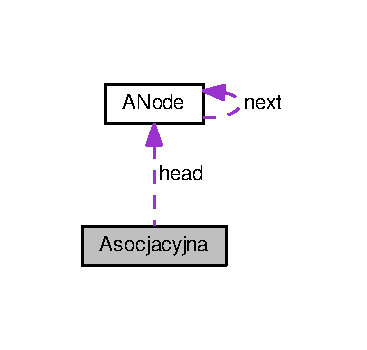
\includegraphics[width=176pt]{struct_asocjacyjna__coll__graph}
\end{center}
\end{figure}
\subsection*{Metody publiczne}
\begin{DoxyCompactItemize}
\item 
\hyperlink{struct_asocjacyjna_a1c65a8bcfb084dcdfa205b052fefd141}{Asocjacyjna} ()
\begin{DoxyCompactList}\small\item\em Konstruktor bezparametryczny obiektu \hyperlink{struct_asocjacyjna}{Asocjacyjna}. \end{DoxyCompactList}\item 
\hyperlink{struct_asocjacyjna_ae618986071c8d141f00df9d6319c0553}{Asocjacyjna} (const \hyperlink{struct_asocjacyjna}{Asocjacyjna} \&\-\_\-l)
\begin{DoxyCompactList}\small\item\em Konstruktor paramteryczny obiektu \hyperlink{struct_asocjacyjna}{Asocjacyjna}. \end{DoxyCompactList}\item 
\hyperlink{struct_asocjacyjna_aa33745fa9b42796199d58f29fa0cd8f0}{$\sim$\-Asocjacyjna} ()
\begin{DoxyCompactList}\small\item\em Destruktor obiektu \hyperlink{struct_asocjacyjna}{Asocjacyjna}. \end{DoxyCompactList}\item 
\hyperlink{struct_asocjacyjna}{Asocjacyjna} \& \hyperlink{struct_asocjacyjna_a23146fc43ca564cf2bf10c326800ffc6}{operator=} (const \hyperlink{struct_asocjacyjna}{Asocjacyjna} \&\-\_\-l)
\begin{DoxyCompactList}\small\item\em Przeladowanie operatora przypisania. Sluzy do wstawiania do klasy elementow innego obiektu tego samego typu. \end{DoxyCompactList}\item 
int \& \hyperlink{struct_asocjacyjna_a91b887ca6ab387a9649d80f6b892b70f}{operator\mbox{[}$\,$\mbox{]}} (const char $\ast$\-\_\-key)
\begin{DoxyCompactList}\small\item\em Przeladowanie operatora nawiasu kwadratowego. Sluzy do wpisywania klucza oraz wartosci. \end{DoxyCompactList}\end{DoxyCompactItemize}
\subsection*{Metody chronione}
\begin{DoxyCompactItemize}
\item 
void \hyperlink{struct_asocjacyjna_a9209f79af7b566f327c8c83f6b879f8b}{clear} ()
\begin{DoxyCompactList}\small\item\em Metoda usuwania zawartosci listy. \end{DoxyCompactList}\item 
\hyperlink{struct_a_node}{A\-Node} $\ast$ \hyperlink{struct_asocjacyjna_a6a9788d36521b4a89db3ab5a0110456f}{find} (const char $\ast$\-\_\-key) const 
\begin{DoxyCompactList}\small\item\em Metoda wyszukiwania elementu o podanym kluczu. \end{DoxyCompactList}\item 
void \hyperlink{struct_asocjacyjna_a0da4ccec0addd9aa1c4309e306994011}{insert} (const char $\ast$\-\_\-key, int \-\_\-value)
\begin{DoxyCompactList}\small\item\em Metoda wstawiania nowej pary klucz-\/wartosc. \end{DoxyCompactList}\item 
void \hyperlink{struct_asocjacyjna_ab6205ed432a156f99cd8b69f6931adb7}{swap} (\hyperlink{struct_asocjacyjna}{Asocjacyjna} \&\-\_\-l)
\begin{DoxyCompactList}\small\item\em Metoda zamiany dwoch list. \end{DoxyCompactList}\end{DoxyCompactItemize}
\subsection*{Atrybuty prywatne}
\begin{DoxyCompactItemize}
\item 
\hyperlink{struct_a_node}{A\-Node} $\ast$ \hyperlink{struct_asocjacyjna_adf1a2a6a5b0b6254122050bbe8c69046}{head}
\begin{DoxyCompactList}\small\item\em Wskaznik na pierwsza pare klucz-\/wartosc. \end{DoxyCompactList}\end{DoxyCompactItemize}
\subsection*{Przyjaciele}
\begin{DoxyCompactItemize}
\item 
std\-::ostream \& \hyperlink{struct_asocjacyjna_ad2f948e16f11dff58951c8104450742e}{operator$<$$<$} (std\-::ostream \&\-\_\-stream, \hyperlink{struct_asocjacyjna}{Asocjacyjna} \&\-\_\-l)
\begin{DoxyCompactList}\small\item\em Przeladowanie operatora przesuniecia bitowego. Sluzy do wypisywania zawartosci listy na strumien wyjsciowy. \end{DoxyCompactList}\end{DoxyCompactItemize}


\subsection{Opis szczegółowy}


Definicja w linii 54 pliku asocjacyjna.\-hh.



\subsection{Dokumentacja konstruktora i destruktora}
\hypertarget{struct_asocjacyjna_a1c65a8bcfb084dcdfa205b052fefd141}{\index{Asocjacyjna@{Asocjacyjna}!Asocjacyjna@{Asocjacyjna}}
\index{Asocjacyjna@{Asocjacyjna}!Asocjacyjna@{Asocjacyjna}}
\subsubsection[{Asocjacyjna}]{\setlength{\rightskip}{0pt plus 5cm}Asocjacyjna\-::\-Asocjacyjna (
\begin{DoxyParamCaption}
{}
\end{DoxyParamCaption}
)}}\label{struct_asocjacyjna_a1c65a8bcfb084dcdfa205b052fefd141}


Definicja w linii 35 pliku asocjacyjna.\-cpp.

\hypertarget{struct_asocjacyjna_ae618986071c8d141f00df9d6319c0553}{\index{Asocjacyjna@{Asocjacyjna}!Asocjacyjna@{Asocjacyjna}}
\index{Asocjacyjna@{Asocjacyjna}!Asocjacyjna@{Asocjacyjna}}
\subsubsection[{Asocjacyjna}]{\setlength{\rightskip}{0pt plus 5cm}Asocjacyjna\-::\-Asocjacyjna (
\begin{DoxyParamCaption}
\item[{const {\bf Asocjacyjna} \&}]{\-\_\-l}
\end{DoxyParamCaption}
)}}\label{struct_asocjacyjna_ae618986071c8d141f00df9d6319c0553}

\begin{DoxyParams}[1]{Parametry}
\mbox{\tt in}  & {\em \-\_\-l} & -\/ referencja do listy. \\
\hline
\end{DoxyParams}


Definicja w linii 41 pliku asocjacyjna.\-cpp.



Oto graf wywołań dla tej funkcji\-:
\nopagebreak
\begin{figure}[H]
\begin{center}
\leavevmode
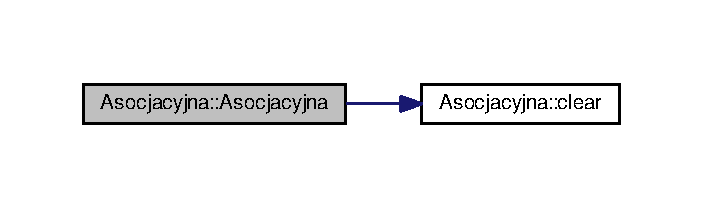
\includegraphics[width=338pt]{struct_asocjacyjna_ae618986071c8d141f00df9d6319c0553_cgraph}
\end{center}
\end{figure}


\hypertarget{struct_asocjacyjna_aa33745fa9b42796199d58f29fa0cd8f0}{\index{Asocjacyjna@{Asocjacyjna}!$\sim$\-Asocjacyjna@{$\sim$\-Asocjacyjna}}
\index{$\sim$\-Asocjacyjna@{$\sim$\-Asocjacyjna}!Asocjacyjna@{Asocjacyjna}}
\subsubsection[{$\sim$\-Asocjacyjna}]{\setlength{\rightskip}{0pt plus 5cm}Asocjacyjna\-::$\sim$\-Asocjacyjna (
\begin{DoxyParamCaption}
{}
\end{DoxyParamCaption}
)}}\label{struct_asocjacyjna_aa33745fa9b42796199d58f29fa0cd8f0}


Definicja w linii 62 pliku asocjacyjna.\-cpp.



Oto graf wywołań dla tej funkcji\-:
\nopagebreak
\begin{figure}[H]
\begin{center}
\leavevmode
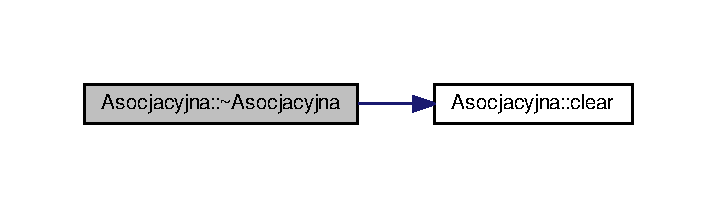
\includegraphics[width=344pt]{struct_asocjacyjna_aa33745fa9b42796199d58f29fa0cd8f0_cgraph}
\end{center}
\end{figure}




\subsection{Dokumentacja funkcji składowych}
\hypertarget{struct_asocjacyjna_a9209f79af7b566f327c8c83f6b879f8b}{\index{Asocjacyjna@{Asocjacyjna}!clear@{clear}}
\index{clear@{clear}!Asocjacyjna@{Asocjacyjna}}
\subsubsection[{clear}]{\setlength{\rightskip}{0pt plus 5cm}void Asocjacyjna\-::clear (
\begin{DoxyParamCaption}
{}
\end{DoxyParamCaption}
)\hspace{0.3cm}{\ttfamily [protected]}}}\label{struct_asocjacyjna_a9209f79af7b566f327c8c83f6b879f8b}


Definicja w linii 94 pliku asocjacyjna.\-cpp.



Oto graf wywoływań tej funkcji\-:
\nopagebreak
\begin{figure}[H]
\begin{center}
\leavevmode
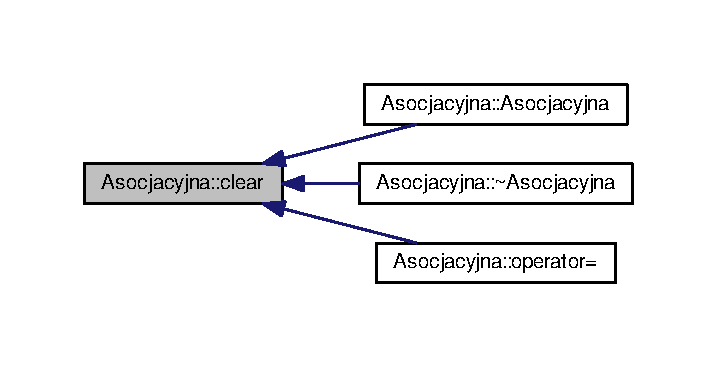
\includegraphics[width=344pt]{struct_asocjacyjna_a9209f79af7b566f327c8c83f6b879f8b_icgraph}
\end{center}
\end{figure}


\hypertarget{struct_asocjacyjna_a6a9788d36521b4a89db3ab5a0110456f}{\index{Asocjacyjna@{Asocjacyjna}!find@{find}}
\index{find@{find}!Asocjacyjna@{Asocjacyjna}}
\subsubsection[{find}]{\setlength{\rightskip}{0pt plus 5cm}{\bf A\-Node} $\ast$ Asocjacyjna\-::find (
\begin{DoxyParamCaption}
\item[{const char $\ast$}]{\-\_\-key}
\end{DoxyParamCaption}
) const\hspace{0.3cm}{\ttfamily [protected]}}}\label{struct_asocjacyjna_a6a9788d36521b4a89db3ab5a0110456f}

\begin{DoxyParams}[1]{Parametry}
\mbox{\tt in}  & {\em \-\_\-key} & -\/ wskaznik na wyszukiwany klucz. \\
\hline
\end{DoxyParams}
\begin{DoxyReturn}{Zwraca}
wskaznik na szukana pare klucz-\/wartosc, nullprt gdy nie znalezniono klucza. 
\end{DoxyReturn}


Definicja w linii 121 pliku asocjacyjna.\-cpp.



Oto graf wywoływań tej funkcji\-:
\nopagebreak
\begin{figure}[H]
\begin{center}
\leavevmode
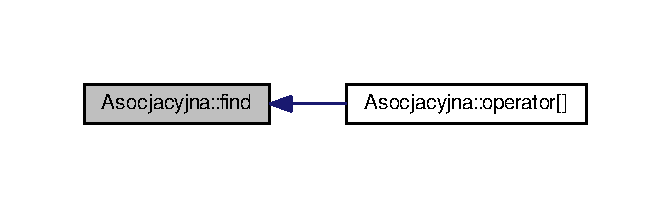
\includegraphics[width=322pt]{struct_asocjacyjna_a6a9788d36521b4a89db3ab5a0110456f_icgraph}
\end{center}
\end{figure}


\hypertarget{struct_asocjacyjna_a0da4ccec0addd9aa1c4309e306994011}{\index{Asocjacyjna@{Asocjacyjna}!insert@{insert}}
\index{insert@{insert}!Asocjacyjna@{Asocjacyjna}}
\subsubsection[{insert}]{\setlength{\rightskip}{0pt plus 5cm}void Asocjacyjna\-::insert (
\begin{DoxyParamCaption}
\item[{const char $\ast$}]{\-\_\-key, }
\item[{int}]{\-\_\-value}
\end{DoxyParamCaption}
)\hspace{0.3cm}{\ttfamily [protected]}}}\label{struct_asocjacyjna_a0da4ccec0addd9aa1c4309e306994011}

\begin{DoxyParams}[1]{Parametry}
\mbox{\tt in}  & {\em \-\_\-key} & -\/ wskaznik na klucz. \\
\hline
\mbox{\tt in}  & {\em \-\_\-value} & -\/ wartosc klucza. \\
\hline
\end{DoxyParams}


Definicja w linii 104 pliku asocjacyjna.\-cpp.



Oto graf wywoływań tej funkcji\-:
\nopagebreak
\begin{figure}[H]
\begin{center}
\leavevmode
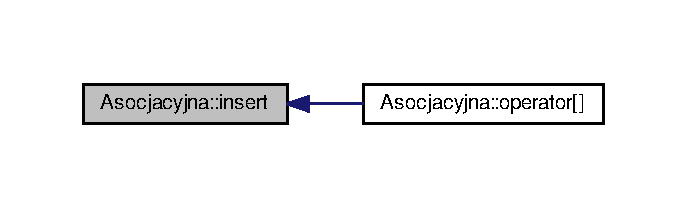
\includegraphics[width=330pt]{struct_asocjacyjna_a0da4ccec0addd9aa1c4309e306994011_icgraph}
\end{center}
\end{figure}


\hypertarget{struct_asocjacyjna_a23146fc43ca564cf2bf10c326800ffc6}{\index{Asocjacyjna@{Asocjacyjna}!operator=@{operator=}}
\index{operator=@{operator=}!Asocjacyjna@{Asocjacyjna}}
\subsubsection[{operator=}]{\setlength{\rightskip}{0pt plus 5cm}{\bf Asocjacyjna} \& Asocjacyjna\-::operator= (
\begin{DoxyParamCaption}
\item[{const {\bf Asocjacyjna} \&}]{\-\_\-l}
\end{DoxyParamCaption}
)}}\label{struct_asocjacyjna_a23146fc43ca564cf2bf10c326800ffc6}

\begin{DoxyParams}[1]{Parametry}
\mbox{\tt in}  & {\em \-\_\-l} & -\/ referencja do listy. \\
\hline
\end{DoxyParams}
\begin{DoxyReturn}{Zwraca}
wskaznik na obiekt. 
\end{DoxyReturn}


Definicja w linii 68 pliku asocjacyjna.\-cpp.



Oto graf wywołań dla tej funkcji\-:
\nopagebreak
\begin{figure}[H]
\begin{center}
\leavevmode
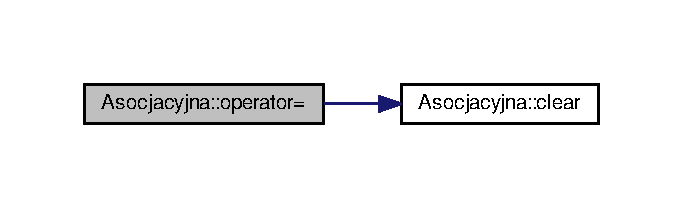
\includegraphics[width=328pt]{struct_asocjacyjna_a23146fc43ca564cf2bf10c326800ffc6_cgraph}
\end{center}
\end{figure}


\hypertarget{struct_asocjacyjna_a91b887ca6ab387a9649d80f6b892b70f}{\index{Asocjacyjna@{Asocjacyjna}!operator\mbox{[}$\,$\mbox{]}@{operator[]}}
\index{operator\mbox{[}$\,$\mbox{]}@{operator[]}!Asocjacyjna@{Asocjacyjna}}
\subsubsection[{operator[]}]{\setlength{\rightskip}{0pt plus 5cm}int \& Asocjacyjna\-::operator\mbox{[}$\,$\mbox{]} (
\begin{DoxyParamCaption}
\item[{const char $\ast$}]{\-\_\-key}
\end{DoxyParamCaption}
)}}\label{struct_asocjacyjna_a91b887ca6ab387a9649d80f6b892b70f}

\begin{DoxyParams}[1]{Parametry}
\mbox{\tt in}  & {\em \-\_\-key} & -\/ wskaznik na klucz. \\
\hline
\end{DoxyParams}
\begin{DoxyReturn}{Zwraca}
wartosc klucza. 
\end{DoxyReturn}


Definicja w linii 133 pliku asocjacyjna.\-cpp.



Oto graf wywołań dla tej funkcji\-:
\nopagebreak
\begin{figure}[H]
\begin{center}
\leavevmode
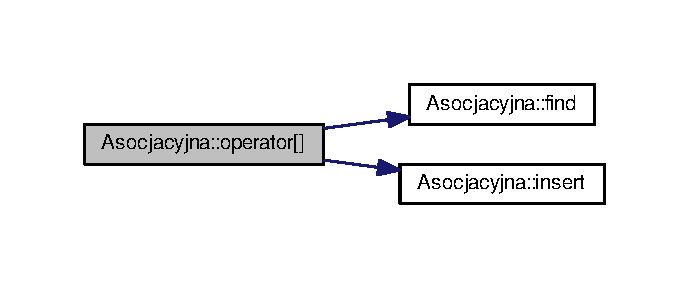
\includegraphics[width=330pt]{struct_asocjacyjna_a91b887ca6ab387a9649d80f6b892b70f_cgraph}
\end{center}
\end{figure}


\hypertarget{struct_asocjacyjna_ab6205ed432a156f99cd8b69f6931adb7}{\index{Asocjacyjna@{Asocjacyjna}!swap@{swap}}
\index{swap@{swap}!Asocjacyjna@{Asocjacyjna}}
\subsubsection[{swap}]{\setlength{\rightskip}{0pt plus 5cm}void Asocjacyjna\-::swap (
\begin{DoxyParamCaption}
\item[{{\bf Asocjacyjna} \&}]{\-\_\-l}
\end{DoxyParamCaption}
)\hspace{0.3cm}{\ttfamily [protected]}}}\label{struct_asocjacyjna_ab6205ed432a156f99cd8b69f6931adb7}

\begin{DoxyParams}[1]{Parametry}
\mbox{\tt in}  & {\em \-\_\-l} & -\/ referencja do listy. \\
\hline
\end{DoxyParams}


Definicja w linii 113 pliku asocjacyjna.\-cpp.



\subsection{Dokumentacja przyjaciół i funkcji związanych}
\hypertarget{struct_asocjacyjna_ad2f948e16f11dff58951c8104450742e}{\index{Asocjacyjna@{Asocjacyjna}!operator$<$$<$@{operator$<$$<$}}
\index{operator$<$$<$@{operator$<$$<$}!Asocjacyjna@{Asocjacyjna}}
\subsubsection[{operator$<$$<$}]{\setlength{\rightskip}{0pt plus 5cm}std\-::ostream\& operator$<$$<$ (
\begin{DoxyParamCaption}
\item[{std\-::ostream \&}]{\-\_\-stream, }
\item[{{\bf Asocjacyjna} \&}]{\-\_\-l}
\end{DoxyParamCaption}
)\hspace{0.3cm}{\ttfamily [friend]}}}\label{struct_asocjacyjna_ad2f948e16f11dff58951c8104450742e}

\begin{DoxyParams}[1]{Parametry}
\mbox{\tt in}  & {\em \-\_\-stream} & -\/ referencja do strumienia wyjsciowego. \\
\hline
\mbox{\tt in}  & {\em \-\_\-l} & -\/ referencja do listy. \\
\hline
\end{DoxyParams}
\begin{DoxyReturn}{Zwraca}
strumien wyjsciowy. 
\end{DoxyReturn}


Definicja w linii 146 pliku asocjacyjna.\-cpp.



\subsection{Dokumentacja atrybutów składowych}
\hypertarget{struct_asocjacyjna_adf1a2a6a5b0b6254122050bbe8c69046}{\index{Asocjacyjna@{Asocjacyjna}!head@{head}}
\index{head@{head}!Asocjacyjna@{Asocjacyjna}}
\subsubsection[{head}]{\setlength{\rightskip}{0pt plus 5cm}{\bf A\-Node}$\ast$ Asocjacyjna\-::head\hspace{0.3cm}{\ttfamily [private]}}}\label{struct_asocjacyjna_adf1a2a6a5b0b6254122050bbe8c69046}


Definicja w linii 59 pliku asocjacyjna.\-hh.



Dokumentacja dla tej struktury została wygenerowana z plików\-:\begin{DoxyCompactItemize}
\item 
\hyperlink{asocjacyjna_8hh}{asocjacyjna.\-hh}\item 
\hyperlink{asocjacyjna_8cpp}{asocjacyjna.\-cpp}\end{DoxyCompactItemize}

\hypertarget{class_benchmark}{\section{Dokumentacja klasy Benchmark}
\label{class_benchmark}\index{Benchmark@{Benchmark}}
}


Klasa \hyperlink{class_benchmark}{Benchmark} modelujaca program benchmarkujacy. Obiekt tego typu reprezentuje program sprawdzajacy szybkosc wykonywania algorytmow.  




{\ttfamily \#include $<$benchmark.\-hh$>$}



Diagram dziedziczenia dla Benchmark\nopagebreak
\begin{figure}[H]
\begin{center}
\leavevmode
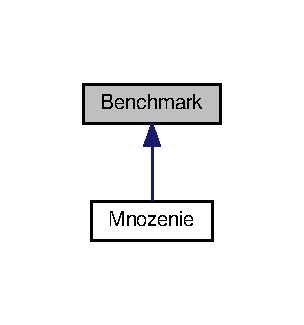
\includegraphics[width=350pt]{class_benchmark__inherit__graph}
\end{center}
\end{figure}
\subsection*{Metody publiczne}
\begin{DoxyCompactItemize}
\item 
\hyperlink{class_benchmark_acfca497989836a688d44477802e822d8}{Benchmark} ()
\begin{DoxyCompactList}\small\item\em Konstrukor obiektu \hyperlink{class_benchmark}{Benchmark}. \end{DoxyCompactList}\item 
\hyperlink{class_benchmark_a20476e07f09e2b20ed3e9a7f13a570e6}{$\sim$\-Benchmark} ()
\begin{DoxyCompactList}\small\item\em Destruktor obiektu \hyperlink{class_benchmark}{Benchmark}. \end{DoxyCompactList}\item 
virtual void \hyperlink{class_benchmark_a900bc0d26c2ed6aa45afe4d5b295ccd1}{test\-Algorithm} (\hyperlink{class_benchmark}{Benchmark} $\ast$\-\_\-algorithm, int \-\_\-n) const 
\begin{DoxyCompactList}\small\item\em Metoda testowania algorytmu. Metoda sluzy to testowania szybkosci dzialania algorytmu. Wykonuje testowany algorytm dla 5 kolejnych ilosci elementow. Wykonanie algorytmu dla danego zestawu liczb powtarza dwa razy i usrednia wynik. Otrzymany czas wraz z iloscia testowanych danych zapisuje w pliku ret\-\_\-data.\-txt. \end{DoxyCompactList}\item 
virtual void \hyperlink{class_benchmark_a6363894c058e8bfe146de09d7126b29c}{run\-Algorithm} (int \-\_\-border)
\begin{DoxyCompactList}\small\item\em Metoda uruchamiania algorytmu. Metoda sluzy do wykonywania danego algorytmu. W klasie \hyperlink{class_benchmark}{Benchmark} nie ma konkretnego dzialania. \end{DoxyCompactList}\end{DoxyCompactItemize}
\subsection*{Atrybuty prywatne}
\begin{DoxyCompactItemize}
\item 
std\-::string \hyperlink{class_benchmark_aee0beda65009e7334d34c5957f78c49a}{nazwy} \mbox{[}4\mbox{]} = \{\char`\"{}ret\-\_\-data1.\-txt\char`\"{}, \char`\"{}ret\-\_\-data2.\-txt\char`\"{}, \char`\"{}ret\-\_\-data3.\-txt\char`\"{}, \char`\"{}ret\-\_\-data4.\-txt\char`\"{}\}
\begin{DoxyCompactList}\small\item\em Tablica stringow przechowujaca nazwy plikow do zapisu. \end{DoxyCompactList}\end{DoxyCompactItemize}


\subsection{Opis szczegółowy}


Definicja w linii 11 pliku benchmark.\-hh.



\subsection{Dokumentacja konstruktora i destruktora}
\hypertarget{class_benchmark_acfca497989836a688d44477802e822d8}{\index{Benchmark@{Benchmark}!Benchmark@{Benchmark}}
\index{Benchmark@{Benchmark}!Benchmark@{Benchmark}}
\subsubsection[{Benchmark}]{\setlength{\rightskip}{0pt plus 5cm}Benchmark\-::\-Benchmark (
\begin{DoxyParamCaption}
{}
\end{DoxyParamCaption}
)\hspace{0.3cm}{\ttfamily [inline]}}}\label{class_benchmark_acfca497989836a688d44477802e822d8}


Definicja w linii 23 pliku benchmark.\-hh.

\hypertarget{class_benchmark_a20476e07f09e2b20ed3e9a7f13a570e6}{\index{Benchmark@{Benchmark}!$\sim$\-Benchmark@{$\sim$\-Benchmark}}
\index{$\sim$\-Benchmark@{$\sim$\-Benchmark}!Benchmark@{Benchmark}}
\subsubsection[{$\sim$\-Benchmark}]{\setlength{\rightskip}{0pt plus 5cm}Benchmark\-::$\sim$\-Benchmark (
\begin{DoxyParamCaption}
{}
\end{DoxyParamCaption}
)\hspace{0.3cm}{\ttfamily [inline]}}}\label{class_benchmark_a20476e07f09e2b20ed3e9a7f13a570e6}


Definicja w linii 28 pliku benchmark.\-hh.



\subsection{Dokumentacja funkcji składowych}
\hypertarget{class_benchmark_a6363894c058e8bfe146de09d7126b29c}{\index{Benchmark@{Benchmark}!run\-Algorithm@{run\-Algorithm}}
\index{run\-Algorithm@{run\-Algorithm}!Benchmark@{Benchmark}}
\subsubsection[{run\-Algorithm}]{\setlength{\rightskip}{0pt plus 5cm}virtual void Benchmark\-::run\-Algorithm (
\begin{DoxyParamCaption}
\item[{int}]{\-\_\-border}
\end{DoxyParamCaption}
)\hspace{0.3cm}{\ttfamily [inline]}, {\ttfamily [virtual]}}}\label{class_benchmark_a6363894c058e8bfe146de09d7126b29c}

\begin{DoxyParams}[1]{Parametry}
\mbox{\tt in}  & {\em \-\_\-border} & -\/ ilosc elementow dla ktorych algorytm ma wykonac swoje dzialanie. \\
\hline
\end{DoxyParams}


Reimplementowana w \hyperlink{class_algorithm2_a409e58d5fb0b6d2407cc986cf163703b}{Algorithm2}, \hyperlink{class_algorithm_kolejka_ae9da3f1862fd90feb4a3c1d6b4f3dd8d}{Algorithm\-Kolejka}, \hyperlink{class_algorithm_lista_a5c41dbbd3ae7a9ac34edec1a51bc8eb1}{Algorithm\-Lista} i \hyperlink{class_algorithm_stos_a889f7150ae3651b40e5acca7542dbbd1}{Algorithm\-Stos}.



Definicja w linii 48 pliku benchmark.\-hh.



Oto graf wywoływań tej funkcji\-:\nopagebreak
\begin{figure}[H]
\begin{center}
\leavevmode
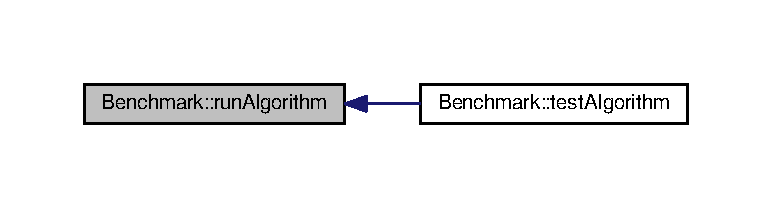
\includegraphics[width=350pt]{class_benchmark_a6363894c058e8bfe146de09d7126b29c_icgraph}
\end{center}
\end{figure}


\hypertarget{class_benchmark_a900bc0d26c2ed6aa45afe4d5b295ccd1}{\index{Benchmark@{Benchmark}!test\-Algorithm@{test\-Algorithm}}
\index{test\-Algorithm@{test\-Algorithm}!Benchmark@{Benchmark}}
\subsubsection[{test\-Algorithm}]{\setlength{\rightskip}{0pt plus 5cm}void Benchmark\-::test\-Algorithm (
\begin{DoxyParamCaption}
\item[{{\bf Benchmark} $\ast$}]{\-\_\-algorithm, }
\item[{int}]{\-\_\-n}
\end{DoxyParamCaption}
) const\hspace{0.3cm}{\ttfamily [virtual]}}}\label{class_benchmark_a900bc0d26c2ed6aa45afe4d5b295ccd1}

\begin{DoxyParams}[1]{Parametry}
\mbox{\tt in}  & {\em \-\_\-algorithm} & -\/ testowany algorytm. \\
\hline
\mbox{\tt in}  & {\em \-\_\-n} & -\/ indeks nazwy pliku \\
\hline
\end{DoxyParams}


Definicja w linii 12 pliku benchmark.\-cpp.



Oto graf wywołań dla tej funkcji\-:\nopagebreak
\begin{figure}[H]
\begin{center}
\leavevmode
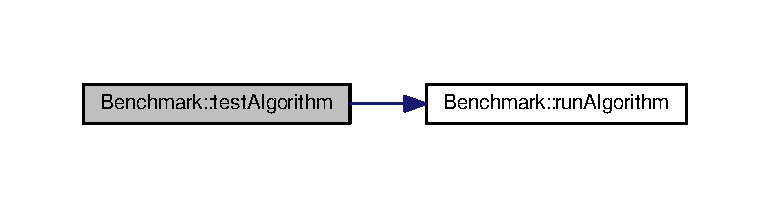
\includegraphics[width=350pt]{class_benchmark_a900bc0d26c2ed6aa45afe4d5b295ccd1_cgraph}
\end{center}
\end{figure}




\subsection{Dokumentacja atrybutów składowych}
\hypertarget{class_benchmark_aee0beda65009e7334d34c5957f78c49a}{\index{Benchmark@{Benchmark}!nazwy@{nazwy}}
\index{nazwy@{nazwy}!Benchmark@{Benchmark}}
\subsubsection[{nazwy}]{\setlength{\rightskip}{0pt plus 5cm}std\-::string Benchmark\-::nazwy\mbox{[}4\mbox{]} = \{\char`\"{}ret\-\_\-data1.\-txt\char`\"{}, \char`\"{}ret\-\_\-data2.\-txt\char`\"{}, \char`\"{}ret\-\_\-data3.\-txt\char`\"{}, \char`\"{}ret\-\_\-data4.\-txt\char`\"{}\}\hspace{0.3cm}{\ttfamily [private]}}}\label{class_benchmark_aee0beda65009e7334d34c5957f78c49a}


Definicja w linii 16 pliku benchmark.\-hh.



Dokumentacja dla tej klasy została wygenerowana z plików\-:\begin{DoxyCompactItemize}
\item 
\hyperlink{benchmark_8hh}{benchmark.\-hh}\item 
\hyperlink{benchmark_8cpp}{benchmark.\-cpp}\end{DoxyCompactItemize}

\hypertarget{struct_binary_tree}{\section{Dokumentacja struktury Binary\-Tree}
\label{struct_binary_tree}\index{Binary\-Tree@{Binary\-Tree}}
}


{\ttfamily \#include $<$binary\-\_\-tree.\-hh$>$}



Diagram współpracy dla Binary\-Tree\-:
\nopagebreak
\begin{figure}[H]
\begin{center}
\leavevmode
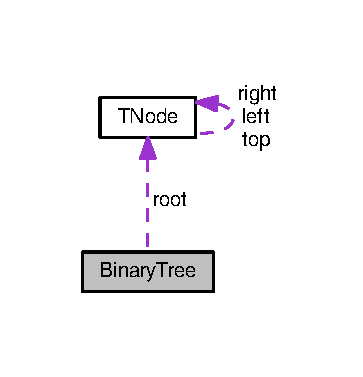
\includegraphics[width=174pt]{struct_binary_tree__coll__graph}
\end{center}
\end{figure}
\subsection*{Metody publiczne}
\begin{DoxyCompactItemize}
\item 
\hyperlink{struct_binary_tree_adf45bce605436b26c353b87e27bffe50}{Binary\-Tree} ()
\begin{DoxyCompactList}\small\item\em Konstruktor obiektu \hyperlink{struct_binary_tree}{Binary\-Tree}. \end{DoxyCompactList}\item 
\hyperlink{struct_binary_tree_a48c23a22a8400765d099e0e6fcebc236}{$\sim$\-Binary\-Tree} ()
\begin{DoxyCompactList}\small\item\em Destruktor obiektu \hyperlink{struct_binary_tree}{Binary\-Tree}. \end{DoxyCompactList}\item 
\hyperlink{struct_t_node}{T\-Node} $\ast$ \hyperlink{struct_binary_tree_a478377892185d59a6af540ad1e667898}{look} (int \-\_\-elem)
\begin{DoxyCompactList}\small\item\em Metoda poszukiwania elementu. Metoda sluzy do szukania elementu o danej wartosci. \end{DoxyCompactList}\item 
\hyperlink{struct_t_node}{T\-Node} $\ast$ \hyperlink{struct_binary_tree_a224960241e35019ce084f25632a4dbcd}{min\-\_\-elem} ()
\begin{DoxyCompactList}\small\item\em Metoda poszukiwania najmniejszego elementu. Metoda sluzy do poszukiwania najmniejszego elementu drzewa przez poszukiwanie lewego konca drzewa. \end{DoxyCompactList}\item 
\hyperlink{struct_t_node}{T\-Node} $\ast$ \hyperlink{struct_binary_tree_a858b64e28ff27071b08ec57af7ea1f50}{max\-\_\-elem} ()
\begin{DoxyCompactList}\small\item\em Metoda poszukiwania najwiekszego elementu. Metoda sluzy do poszukiwania najwiekszego elementu drzewa przez poszukiwanie prawego konca drzewa. \end{DoxyCompactList}\item 
void \hyperlink{struct_binary_tree_a2cba03e2583aa1aaba6e610e21fb7521}{add\-\_\-elem} (int \-\_\-elem)
\begin{DoxyCompactList}\small\item\em Metoda dodawania elementu. Metoda sluzy do dodawania elementu o zadanej wartosci. \end{DoxyCompactList}\item 
void \hyperlink{struct_binary_tree_a2c72362db265ea08bb9ab45e285eb4a1}{is\-\_\-\-B\-S\-T} ()
\begin{DoxyCompactList}\small\item\em Metoda sprawdzania struktury drzewa. Metoda sluzy do sprawdzania czy drzewo ma strukture binarnego drzewa poszukiwan. \end{DoxyCompactList}\item 
void \hyperlink{struct_binary_tree_ad0e4ce622ad8abf4dfb0f051e9c9af92}{clear} ()
\begin{DoxyCompactList}\small\item\em Metoda oprozniania drzewa. Metoda sluzy do usuwania wszystkich elementow z drzewa. Wykonuje swoje dzialanie rekurencyjnie. \end{DoxyCompactList}\item 
void \hyperlink{struct_binary_tree_a8f557920c17957b4ae378727ac898c18}{print\-\_\-tree} ()
\begin{DoxyCompactList}\small\item\em Metoda drukowania drzewa. Metoda sluzy do wypisywania wszystkich elementow z drzewa na std out. Wykonuje swoje dzialanie rekurencyjnie. \end{DoxyCompactList}\end{DoxyCompactItemize}
\subsection*{Metody chronione}
\begin{DoxyCompactItemize}
\item 
\hyperlink{struct_t_node}{T\-Node} $\ast$ \hyperlink{struct_binary_tree_a47e590bb37b4b419ac9eff13fb03b6cf}{look} (\hyperlink{struct_t_node}{T\-Node} $\ast$\-\_\-node, int \-\_\-elem)
\begin{DoxyCompactList}\small\item\em Metoda poszukiwania elementu. Metoda sluzy do szukania elementu o danej wartosci. \end{DoxyCompactList}\item 
\hyperlink{struct_t_node}{T\-Node} $\ast$ \hyperlink{struct_binary_tree_a749356c206465c8c4b7ef905a2a75f63}{new\-\_\-node} (int \-\_\-elem)
\begin{DoxyCompactList}\small\item\em Metoda tworzenia komorki. Metoda sluzy do tworzenia komorki o zadanej wartosci. \end{DoxyCompactList}\item 
void \hyperlink{struct_binary_tree_acffce31cb381fa5fd9029e420ec7bceb}{add\-\_\-elem} (\hyperlink{struct_t_node}{T\-Node} $\ast$\-\_\-node, int \-\_\-elem)
\begin{DoxyCompactList}\small\item\em Metoda dodawania elementu. Metoda sluzy do dodawania elementu o zadanej wartosci. \end{DoxyCompactList}\item 
void \hyperlink{struct_binary_tree_a95191528b6584bd3f05e38a91069f050}{is\-\_\-\-B\-S\-T} (\hyperlink{struct_t_node}{T\-Node} $\ast$\-\_\-node)
\begin{DoxyCompactList}\small\item\em Metoda sprawdzania struktury drzewa. Metoda sluzy do sprawdzania czy drzewo ma strukture binarnego drzewa poszukiwan. \end{DoxyCompactList}\item 
void \hyperlink{struct_binary_tree_a71e2586551ccbaff9b2dfcc61c27820f}{clear} (\hyperlink{struct_t_node}{T\-Node} $\ast$\-\_\-node)
\begin{DoxyCompactList}\small\item\em Metoda oprozniania drzewa. Metoda sluzy do usuwania wszystkich elementow z drzewa. Wykonuje swoje dzialanie rekurencyjnie. \end{DoxyCompactList}\item 
void \hyperlink{struct_binary_tree_ae0183134e9d30f5a61869df126e8bc2c}{print\-\_\-tree} (\hyperlink{struct_t_node}{T\-Node} $\ast$\-\_\-node)
\begin{DoxyCompactList}\small\item\em Metoda drukowania drzewa. Metoda sluzy do wypisywania wszystkich elementow z drzewa na std out. Wykonuje swoje dzialanie rekurencyjnie. \end{DoxyCompactList}\end{DoxyCompactItemize}
\subsection*{Atrybuty prywatne}
\begin{DoxyCompactItemize}
\item 
\hyperlink{struct_t_node}{T\-Node} $\ast$ \hyperlink{struct_binary_tree_a154cd3336ceeeb98481e70aa973007b4}{root}
\begin{DoxyCompactList}\small\item\em Wskaznik na korzen drzewa. \end{DoxyCompactList}\end{DoxyCompactItemize}


\subsection{Opis szczegółowy}


Definicja w linii 33 pliku binary\-\_\-tree.\-hh.



\subsection{Dokumentacja konstruktora i destruktora}
\hypertarget{struct_binary_tree_adf45bce605436b26c353b87e27bffe50}{\index{Binary\-Tree@{Binary\-Tree}!Binary\-Tree@{Binary\-Tree}}
\index{Binary\-Tree@{Binary\-Tree}!BinaryTree@{Binary\-Tree}}
\subsubsection[{Binary\-Tree}]{\setlength{\rightskip}{0pt plus 5cm}Binary\-Tree\-::\-Binary\-Tree (
\begin{DoxyParamCaption}
{}
\end{DoxyParamCaption}
)\hspace{0.3cm}{\ttfamily [inline]}}}\label{struct_binary_tree_adf45bce605436b26c353b87e27bffe50}


Definicja w linii 89 pliku binary\-\_\-tree.\-hh.

\hypertarget{struct_binary_tree_a48c23a22a8400765d099e0e6fcebc236}{\index{Binary\-Tree@{Binary\-Tree}!$\sim$\-Binary\-Tree@{$\sim$\-Binary\-Tree}}
\index{$\sim$\-Binary\-Tree@{$\sim$\-Binary\-Tree}!BinaryTree@{Binary\-Tree}}
\subsubsection[{$\sim$\-Binary\-Tree}]{\setlength{\rightskip}{0pt plus 5cm}Binary\-Tree\-::$\sim$\-Binary\-Tree (
\begin{DoxyParamCaption}
{}
\end{DoxyParamCaption}
)\hspace{0.3cm}{\ttfamily [inline]}}}\label{struct_binary_tree_a48c23a22a8400765d099e0e6fcebc236}


Definicja w linii 93 pliku binary\-\_\-tree.\-hh.



\subsection{Dokumentacja funkcji składowych}
\hypertarget{struct_binary_tree_acffce31cb381fa5fd9029e420ec7bceb}{\index{Binary\-Tree@{Binary\-Tree}!add\-\_\-elem@{add\-\_\-elem}}
\index{add\-\_\-elem@{add\-\_\-elem}!BinaryTree@{Binary\-Tree}}
\subsubsection[{add\-\_\-elem}]{\setlength{\rightskip}{0pt plus 5cm}void Binary\-Tree\-::add\-\_\-elem (
\begin{DoxyParamCaption}
\item[{{\bf T\-Node} $\ast$}]{\-\_\-node, }
\item[{int}]{\-\_\-elem}
\end{DoxyParamCaption}
)\hspace{0.3cm}{\ttfamily [protected]}}}\label{struct_binary_tree_acffce31cb381fa5fd9029e420ec7bceb}

\begin{DoxyParams}[1]{Parametry}
\mbox{\tt in}  & {\em \-\_\-node} & -\/ wskaznik na komorke. \\
\hline
\mbox{\tt in}  & {\em \-\_\-elem} & -\/ wartosc. \\
\hline
\end{DoxyParams}


Definicja w linii 60 pliku binary\-\_\-tree.\-cpp.



Oto graf wywołań dla tej funkcji\-:
\nopagebreak
\begin{figure}[H]
\begin{center}
\leavevmode
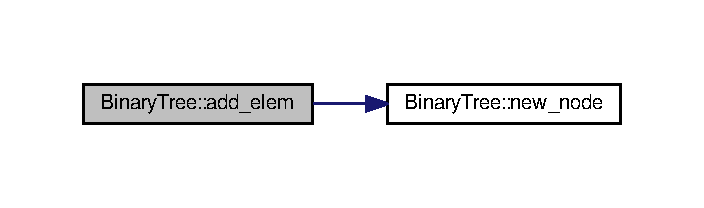
\includegraphics[width=338pt]{struct_binary_tree_acffce31cb381fa5fd9029e420ec7bceb_cgraph}
\end{center}
\end{figure}




Oto graf wywoływań tej funkcji\-:
\nopagebreak
\begin{figure}[H]
\begin{center}
\leavevmode
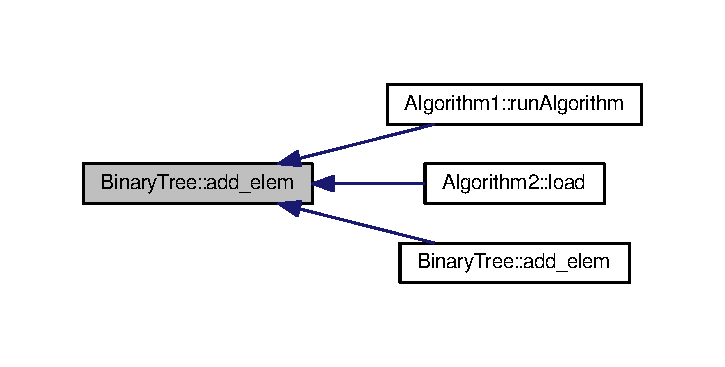
\includegraphics[width=348pt]{struct_binary_tree_acffce31cb381fa5fd9029e420ec7bceb_icgraph}
\end{center}
\end{figure}


\hypertarget{struct_binary_tree_a2cba03e2583aa1aaba6e610e21fb7521}{\index{Binary\-Tree@{Binary\-Tree}!add\-\_\-elem@{add\-\_\-elem}}
\index{add\-\_\-elem@{add\-\_\-elem}!BinaryTree@{Binary\-Tree}}
\subsubsection[{add\-\_\-elem}]{\setlength{\rightskip}{0pt plus 5cm}void Binary\-Tree\-::add\-\_\-elem (
\begin{DoxyParamCaption}
\item[{int}]{\-\_\-elem}
\end{DoxyParamCaption}
)}}\label{struct_binary_tree_a2cba03e2583aa1aaba6e610e21fb7521}

\begin{DoxyParams}[1]{Parametry}
\mbox{\tt in}  & {\em \-\_\-elem} & -\/ wartosc elementu. \\
\hline
\end{DoxyParams}


Definicja w linii 82 pliku binary\-\_\-tree.\-cpp.



Oto graf wywołań dla tej funkcji\-:
\nopagebreak
\begin{figure}[H]
\begin{center}
\leavevmode
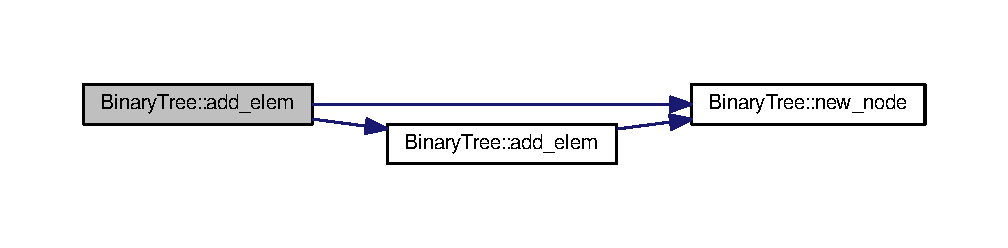
\includegraphics[width=350pt]{struct_binary_tree_a2cba03e2583aa1aaba6e610e21fb7521_cgraph}
\end{center}
\end{figure}


\hypertarget{struct_binary_tree_a71e2586551ccbaff9b2dfcc61c27820f}{\index{Binary\-Tree@{Binary\-Tree}!clear@{clear}}
\index{clear@{clear}!BinaryTree@{Binary\-Tree}}
\subsubsection[{clear}]{\setlength{\rightskip}{0pt plus 5cm}void Binary\-Tree\-::clear (
\begin{DoxyParamCaption}
\item[{{\bf T\-Node} $\ast$}]{\-\_\-node}
\end{DoxyParamCaption}
)\hspace{0.3cm}{\ttfamily [protected]}}}\label{struct_binary_tree_a71e2586551ccbaff9b2dfcc61c27820f}

\begin{DoxyParams}[1]{Parametry}
\mbox{\tt in}  & {\em \-\_\-node} & -\/ wskaznik na startowa komorke. \\
\hline
\end{DoxyParams}


Definicja w linii 104 pliku binary\-\_\-tree.\-cpp.



Oto graf wywołań dla tej funkcji\-:
\nopagebreak
\begin{figure}[H]
\begin{center}
\leavevmode
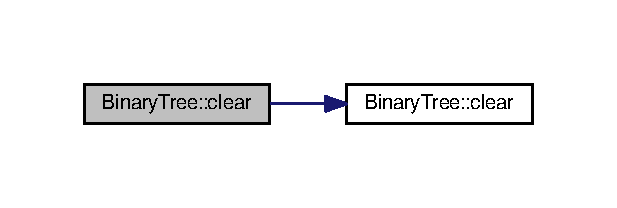
\includegraphics[width=296pt]{struct_binary_tree_a71e2586551ccbaff9b2dfcc61c27820f_cgraph}
\end{center}
\end{figure}




Oto graf wywoływań tej funkcji\-:
\nopagebreak
\begin{figure}[H]
\begin{center}
\leavevmode
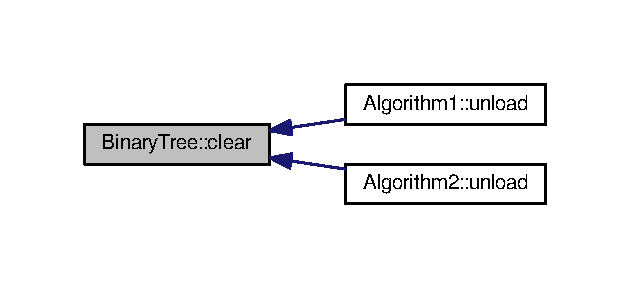
\includegraphics[width=302pt]{struct_binary_tree_a71e2586551ccbaff9b2dfcc61c27820f_icgraph}
\end{center}
\end{figure}


\hypertarget{struct_binary_tree_ad0e4ce622ad8abf4dfb0f051e9c9af92}{\index{Binary\-Tree@{Binary\-Tree}!clear@{clear}}
\index{clear@{clear}!BinaryTree@{Binary\-Tree}}
\subsubsection[{clear}]{\setlength{\rightskip}{0pt plus 5cm}void Binary\-Tree\-::clear (
\begin{DoxyParamCaption}
{}
\end{DoxyParamCaption}
)}}\label{struct_binary_tree_ad0e4ce622ad8abf4dfb0f051e9c9af92}


Definicja w linii 112 pliku binary\-\_\-tree.\-cpp.



Oto graf wywoływań tej funkcji\-:
\nopagebreak
\begin{figure}[H]
\begin{center}
\leavevmode
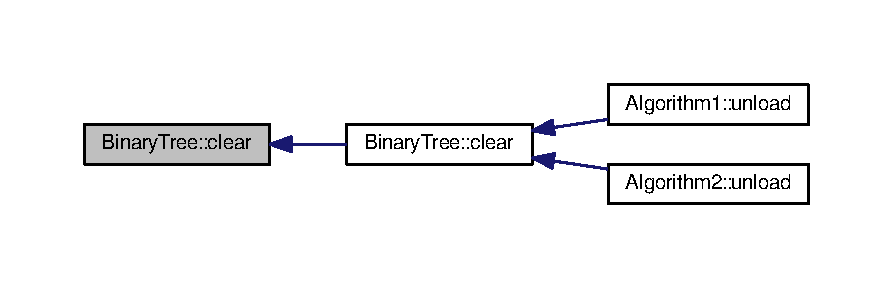
\includegraphics[width=350pt]{struct_binary_tree_ad0e4ce622ad8abf4dfb0f051e9c9af92_icgraph}
\end{center}
\end{figure}


\hypertarget{struct_binary_tree_a95191528b6584bd3f05e38a91069f050}{\index{Binary\-Tree@{Binary\-Tree}!is\-\_\-\-B\-S\-T@{is\-\_\-\-B\-S\-T}}
\index{is\-\_\-\-B\-S\-T@{is\-\_\-\-B\-S\-T}!BinaryTree@{Binary\-Tree}}
\subsubsection[{is\-\_\-\-B\-S\-T}]{\setlength{\rightskip}{0pt plus 5cm}void Binary\-Tree\-::is\-\_\-\-B\-S\-T (
\begin{DoxyParamCaption}
\item[{{\bf T\-Node} $\ast$}]{\-\_\-node}
\end{DoxyParamCaption}
)\hspace{0.3cm}{\ttfamily [protected]}}}\label{struct_binary_tree_a95191528b6584bd3f05e38a91069f050}

\begin{DoxyParams}[1]{Parametry}
\mbox{\tt in}  & {\em \-\_\-node} & -\/ wskaznik na startowa komorke. \\
\hline
\end{DoxyParams}
\hypertarget{struct_binary_tree_a2c72362db265ea08bb9ab45e285eb4a1}{\index{Binary\-Tree@{Binary\-Tree}!is\-\_\-\-B\-S\-T@{is\-\_\-\-B\-S\-T}}
\index{is\-\_\-\-B\-S\-T@{is\-\_\-\-B\-S\-T}!BinaryTree@{Binary\-Tree}}
\subsubsection[{is\-\_\-\-B\-S\-T}]{\setlength{\rightskip}{0pt plus 5cm}void Binary\-Tree\-::is\-\_\-\-B\-S\-T (
\begin{DoxyParamCaption}
{}
\end{DoxyParamCaption}
)}}\label{struct_binary_tree_a2c72362db265ea08bb9ab45e285eb4a1}
\hypertarget{struct_binary_tree_a47e590bb37b4b419ac9eff13fb03b6cf}{\index{Binary\-Tree@{Binary\-Tree}!look@{look}}
\index{look@{look}!BinaryTree@{Binary\-Tree}}
\subsubsection[{look}]{\setlength{\rightskip}{0pt plus 5cm}{\bf T\-Node} $\ast$ Binary\-Tree\-::look (
\begin{DoxyParamCaption}
\item[{{\bf T\-Node} $\ast$}]{\-\_\-node, }
\item[{int}]{\-\_\-elem}
\end{DoxyParamCaption}
)\hspace{0.3cm}{\ttfamily [protected]}}}\label{struct_binary_tree_a47e590bb37b4b419ac9eff13fb03b6cf}

\begin{DoxyParams}[1]{Parametry}
\mbox{\tt in}  & {\em \-\_\-node} & -\/ wskaznik na komorke \\
\hline
\mbox{\tt in}  & {\em \-\_\-elem} & -\/ dodawany element. \\
\hline
\end{DoxyParams}
\begin{DoxyReturn}{Zwraca}
poszukiwana komorka. 
\end{DoxyReturn}


Definicja w linii 15 pliku binary\-\_\-tree.\-cpp.



Oto graf wywoływań tej funkcji\-:
\nopagebreak
\begin{figure}[H]
\begin{center}
\leavevmode
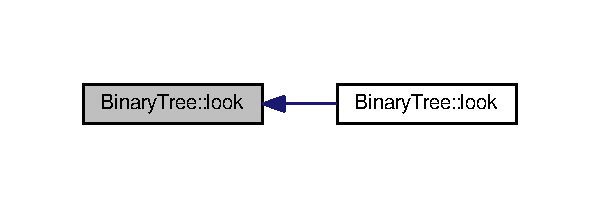
\includegraphics[width=288pt]{struct_binary_tree_a47e590bb37b4b419ac9eff13fb03b6cf_icgraph}
\end{center}
\end{figure}


\hypertarget{struct_binary_tree_a478377892185d59a6af540ad1e667898}{\index{Binary\-Tree@{Binary\-Tree}!look@{look}}
\index{look@{look}!BinaryTree@{Binary\-Tree}}
\subsubsection[{look}]{\setlength{\rightskip}{0pt plus 5cm}{\bf T\-Node} $\ast$ Binary\-Tree\-::look (
\begin{DoxyParamCaption}
\item[{int}]{\-\_\-elem}
\end{DoxyParamCaption}
)}}\label{struct_binary_tree_a478377892185d59a6af540ad1e667898}

\begin{DoxyParams}[1]{Parametry}
\mbox{\tt in}  & {\em \-\_\-elem} & -\/ dodawany element. \\
\hline
\end{DoxyParams}
\begin{DoxyReturn}{Zwraca}
poszukiwana komorka. 
\end{DoxyReturn}


Definicja w linii 26 pliku binary\-\_\-tree.\-cpp.



Oto graf wywołań dla tej funkcji\-:
\nopagebreak
\begin{figure}[H]
\begin{center}
\leavevmode
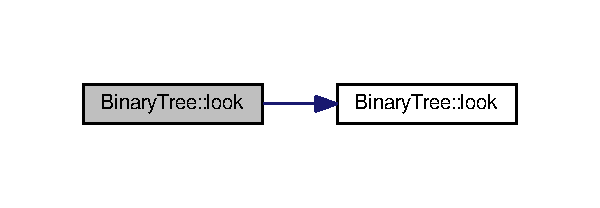
\includegraphics[width=288pt]{struct_binary_tree_a478377892185d59a6af540ad1e667898_cgraph}
\end{center}
\end{figure}


\hypertarget{struct_binary_tree_a858b64e28ff27071b08ec57af7ea1f50}{\index{Binary\-Tree@{Binary\-Tree}!max\-\_\-elem@{max\-\_\-elem}}
\index{max\-\_\-elem@{max\-\_\-elem}!BinaryTree@{Binary\-Tree}}
\subsubsection[{max\-\_\-elem}]{\setlength{\rightskip}{0pt plus 5cm}{\bf T\-Node} $\ast$ Binary\-Tree\-::max\-\_\-elem (
\begin{DoxyParamCaption}
{}
\end{DoxyParamCaption}
)}}\label{struct_binary_tree_a858b64e28ff27071b08ec57af7ea1f50}
\begin{DoxyReturn}{Zwraca}
poszukiwana komorka. 
\end{DoxyReturn}


Definicja w linii 46 pliku binary\-\_\-tree.\-cpp.

\hypertarget{struct_binary_tree_a224960241e35019ce084f25632a4dbcd}{\index{Binary\-Tree@{Binary\-Tree}!min\-\_\-elem@{min\-\_\-elem}}
\index{min\-\_\-elem@{min\-\_\-elem}!BinaryTree@{Binary\-Tree}}
\subsubsection[{min\-\_\-elem}]{\setlength{\rightskip}{0pt plus 5cm}{\bf T\-Node} $\ast$ Binary\-Tree\-::min\-\_\-elem (
\begin{DoxyParamCaption}
{}
\end{DoxyParamCaption}
)}}\label{struct_binary_tree_a224960241e35019ce084f25632a4dbcd}
\begin{DoxyReturn}{Zwraca}
poszukiwana komorka. 
\end{DoxyReturn}


Definicja w linii 38 pliku binary\-\_\-tree.\-cpp.

\hypertarget{struct_binary_tree_a749356c206465c8c4b7ef905a2a75f63}{\index{Binary\-Tree@{Binary\-Tree}!new\-\_\-node@{new\-\_\-node}}
\index{new\-\_\-node@{new\-\_\-node}!BinaryTree@{Binary\-Tree}}
\subsubsection[{new\-\_\-node}]{\setlength{\rightskip}{0pt plus 5cm}{\bf T\-Node} $\ast$ Binary\-Tree\-::new\-\_\-node (
\begin{DoxyParamCaption}
\item[{int}]{\-\_\-elem}
\end{DoxyParamCaption}
)\hspace{0.3cm}{\ttfamily [protected]}}}\label{struct_binary_tree_a749356c206465c8c4b7ef905a2a75f63}

\begin{DoxyParams}[1]{Parametry}
\mbox{\tt in}  & {\em \-\_\-elem} & -\/ wartosc tworzonej komorki. \\
\hline
\end{DoxyParams}
\begin{DoxyReturn}{Zwraca}
wskaznik na tworzona komorke. 
\end{DoxyReturn}


Definicja w linii 54 pliku binary\-\_\-tree.\-cpp.



Oto graf wywoływań tej funkcji\-:
\nopagebreak
\begin{figure}[H]
\begin{center}
\leavevmode
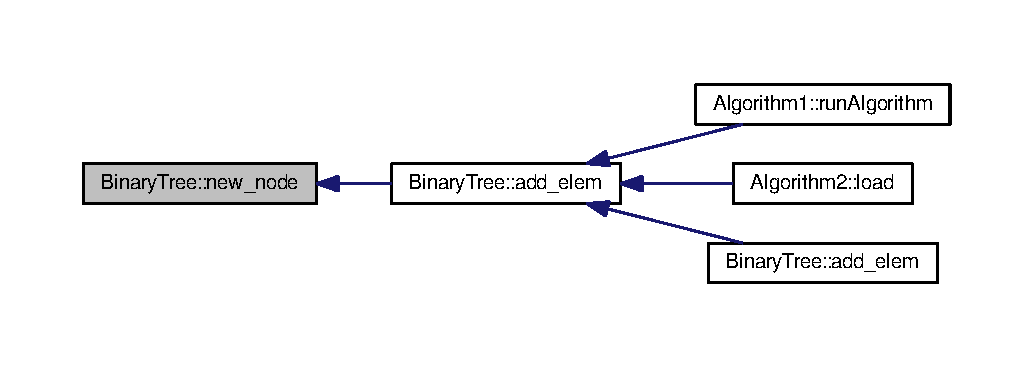
\includegraphics[width=350pt]{struct_binary_tree_a749356c206465c8c4b7ef905a2a75f63_icgraph}
\end{center}
\end{figure}


\hypertarget{struct_binary_tree_ae0183134e9d30f5a61869df126e8bc2c}{\index{Binary\-Tree@{Binary\-Tree}!print\-\_\-tree@{print\-\_\-tree}}
\index{print\-\_\-tree@{print\-\_\-tree}!BinaryTree@{Binary\-Tree}}
\subsubsection[{print\-\_\-tree}]{\setlength{\rightskip}{0pt plus 5cm}void Binary\-Tree\-::print\-\_\-tree (
\begin{DoxyParamCaption}
\item[{{\bf T\-Node} $\ast$}]{\-\_\-node}
\end{DoxyParamCaption}
)\hspace{0.3cm}{\ttfamily [protected]}}}\label{struct_binary_tree_ae0183134e9d30f5a61869df126e8bc2c}

\begin{DoxyParams}[1]{Parametry}
\mbox{\tt in}  & {\em \-\_\-node} & -\/ wskaznik na startowa komorke. \\
\hline
\end{DoxyParams}


Definicja w linii 122 pliku binary\-\_\-tree.\-cpp.



Oto graf wywołań dla tej funkcji\-:
\nopagebreak
\begin{figure}[H]
\begin{center}
\leavevmode
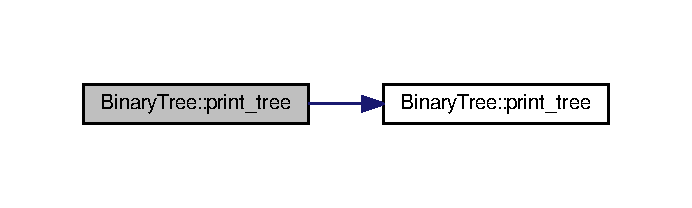
\includegraphics[width=332pt]{struct_binary_tree_ae0183134e9d30f5a61869df126e8bc2c_cgraph}
\end{center}
\end{figure}




Oto graf wywoływań tej funkcji\-:
\nopagebreak
\begin{figure}[H]
\begin{center}
\leavevmode
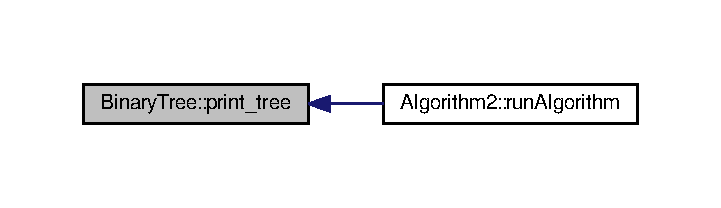
\includegraphics[width=346pt]{struct_binary_tree_ae0183134e9d30f5a61869df126e8bc2c_icgraph}
\end{center}
\end{figure}


\hypertarget{struct_binary_tree_a8f557920c17957b4ae378727ac898c18}{\index{Binary\-Tree@{Binary\-Tree}!print\-\_\-tree@{print\-\_\-tree}}
\index{print\-\_\-tree@{print\-\_\-tree}!BinaryTree@{Binary\-Tree}}
\subsubsection[{print\-\_\-tree}]{\setlength{\rightskip}{0pt plus 5cm}void Binary\-Tree\-::print\-\_\-tree (
\begin{DoxyParamCaption}
{}
\end{DoxyParamCaption}
)}}\label{struct_binary_tree_a8f557920c17957b4ae378727ac898c18}


Definicja w linii 129 pliku binary\-\_\-tree.\-cpp.



Oto graf wywoływań tej funkcji\-:
\nopagebreak
\begin{figure}[H]
\begin{center}
\leavevmode
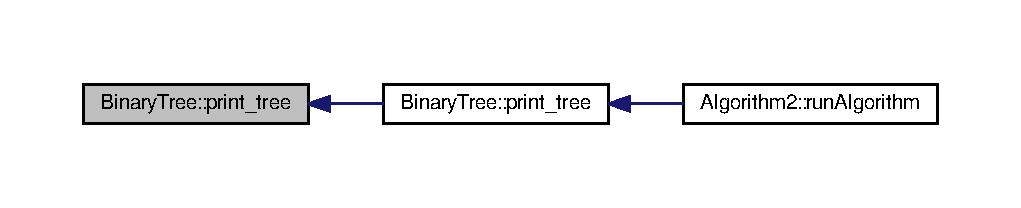
\includegraphics[width=350pt]{struct_binary_tree_a8f557920c17957b4ae378727ac898c18_icgraph}
\end{center}
\end{figure}




\subsection{Dokumentacja atrybutów składowych}
\hypertarget{struct_binary_tree_a154cd3336ceeeb98481e70aa973007b4}{\index{Binary\-Tree@{Binary\-Tree}!root@{root}}
\index{root@{root}!BinaryTree@{Binary\-Tree}}
\subsubsection[{root}]{\setlength{\rightskip}{0pt plus 5cm}{\bf T\-Node}$\ast$ Binary\-Tree\-::root\hspace{0.3cm}{\ttfamily [private]}}}\label{struct_binary_tree_a154cd3336ceeeb98481e70aa973007b4}


Definicja w linii 38 pliku binary\-\_\-tree.\-hh.



Dokumentacja dla tej struktury została wygenerowana z plików\-:\begin{DoxyCompactItemize}
\item 
\hyperlink{binary__tree_8hh}{binary\-\_\-tree.\-hh}\item 
\hyperlink{binary__tree_8cpp}{binary\-\_\-tree.\-cpp}\end{DoxyCompactItemize}

\hypertarget{class_kolejka}{\section{Dokumentacja klasy Kolejka}
\label{class_kolejka}\index{Kolejka@{Kolejka}}
}


Klasa \hyperlink{class_kolejka}{Kolejka} modelujaca strukture danych typu kolejka. Obiekt tego typu reprezentuje strukture danych typu kolejka wraz z operacjami mozliwymi do wykonania na tej strukturze. Dziedziczy po klasie \hyperlink{class_tablicowe}{Tablicowe}.  




{\ttfamily \#include $<$kolejka.\-hh$>$}



Diagram dziedziczenia dla Kolejka\nopagebreak
\begin{figure}[H]
\begin{center}
\leavevmode
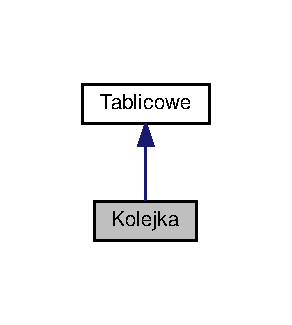
\includegraphics[width=140pt]{class_kolejka__inherit__graph}
\end{center}
\end{figure}


Diagram współpracy dla Kolejka\-:\nopagebreak
\begin{figure}[H]
\begin{center}
\leavevmode
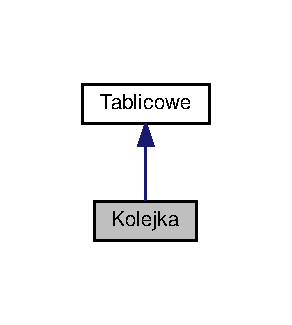
\includegraphics[width=140pt]{class_kolejka__coll__graph}
\end{center}
\end{figure}
\subsection*{Metody publiczne}
\begin{DoxyCompactItemize}
\item 
\hyperlink{class_kolejka_a37c886fdc73dce62b04da0381dec5484}{Kolejka} ()
\begin{DoxyCompactList}\small\item\em Konstruktor obiektu \hyperlink{class_kolejka}{Kolejka}. Tworzy kolejke o domyslnym rozmiarze rownym 8. \end{DoxyCompactList}\item 
\hyperlink{class_kolejka_ac942cc97bf0d2c30d11611c406acc5a8}{Kolejka} (long \-\_\-size)
\begin{DoxyCompactList}\small\item\em Konstruktor parametryczny obiektu \hyperlink{class_kolejka}{Kolejka}. Tworzy kolejke o zadanym rozmiarze rownym \-\_\-size. \end{DoxyCompactList}\item 
\hyperlink{class_kolejka_a352f86ff08cd47be6c35c60bb0f873a6}{$\sim$\-Kolejka} ()
\begin{DoxyCompactList}\small\item\em Destruktor obiektu \hyperlink{class_kolejka}{Kolejka}. \end{DoxyCompactList}\item 
void \hyperlink{class_kolejka_a8f3b0111e85f517d9eadb8ce996d4471}{enqueue} (int \-\_\-elem)
\begin{DoxyCompactList}\small\item\em Metoda dodawnia elementu. Metoda sluzy do dodawania elementu do kolejki. \end{DoxyCompactList}\item 
int \hyperlink{class_kolejka_af23261614bcf242a1934a99688a2debc}{dequeue} ()
\begin{DoxyCompactList}\small\item\em Metoda usuwania elementu. Metoda sluzy do usuwania elementu z kolejki. \end{DoxyCompactList}\end{DoxyCompactItemize}
\subsection*{Metody prywatne}
\begin{DoxyCompactItemize}
\item 
void \hyperlink{class_kolejka_ab4f51f0ec7fef36a85af6cfd1c257427}{increase} ()
\begin{DoxyCompactList}\small\item\em Metoda powiekszania kolejki. Metoda ta zwieksza ilosc pol w kolejce dwukrotnie. \end{DoxyCompactList}\item 
int \hyperlink{class_kolejka_acff09ebfbec69b06c91203bab30d815d}{decrease} ()
\begin{DoxyCompactList}\small\item\em Metoda pomniejszania kolejki. Metoda ta odejmuje od kolejki jedno pole. \end{DoxyCompactList}\end{DoxyCompactItemize}
\subsection*{Dodatkowe Dziedziczone Składowe}


\subsection{Opis szczegółowy}


Definicja w linii 10 pliku kolejka.\-hh.



\subsection{Dokumentacja konstruktora i destruktora}
\hypertarget{class_kolejka_a37c886fdc73dce62b04da0381dec5484}{\index{Kolejka@{Kolejka}!Kolejka@{Kolejka}}
\index{Kolejka@{Kolejka}!Kolejka@{Kolejka}}
\subsubsection[{Kolejka}]{\setlength{\rightskip}{0pt plus 5cm}Kolejka\-::\-Kolejka (
\begin{DoxyParamCaption}
{}
\end{DoxyParamCaption}
)}}\label{class_kolejka_a37c886fdc73dce62b04da0381dec5484}


Definicja w linii 7 pliku kolejka.\-cpp.

\hypertarget{class_kolejka_ac942cc97bf0d2c30d11611c406acc5a8}{\index{Kolejka@{Kolejka}!Kolejka@{Kolejka}}
\index{Kolejka@{Kolejka}!Kolejka@{Kolejka}}
\subsubsection[{Kolejka}]{\setlength{\rightskip}{0pt plus 5cm}Kolejka\-::\-Kolejka (
\begin{DoxyParamCaption}
\item[{long}]{\-\_\-size}
\end{DoxyParamCaption}
)}}\label{class_kolejka_ac942cc97bf0d2c30d11611c406acc5a8}

\begin{DoxyParams}[1]{Parametry}
\mbox{\tt in}  & {\em \-\_\-size} & -\/ startowy rozmiar struktury. \\
\hline
\end{DoxyParams}


Definicja w linii 17 pliku kolejka.\-cpp.

\hypertarget{class_kolejka_a352f86ff08cd47be6c35c60bb0f873a6}{\index{Kolejka@{Kolejka}!$\sim$\-Kolejka@{$\sim$\-Kolejka}}
\index{$\sim$\-Kolejka@{$\sim$\-Kolejka}!Kolejka@{Kolejka}}
\subsubsection[{$\sim$\-Kolejka}]{\setlength{\rightskip}{0pt plus 5cm}Kolejka\-::$\sim$\-Kolejka (
\begin{DoxyParamCaption}
{}
\end{DoxyParamCaption}
)}}\label{class_kolejka_a352f86ff08cd47be6c35c60bb0f873a6}


Definicja w linii 27 pliku kolejka.\-cpp.



\subsection{Dokumentacja funkcji składowych}
\hypertarget{class_kolejka_acff09ebfbec69b06c91203bab30d815d}{\index{Kolejka@{Kolejka}!decrease@{decrease}}
\index{decrease@{decrease}!Kolejka@{Kolejka}}
\subsubsection[{decrease}]{\setlength{\rightskip}{0pt plus 5cm}int Kolejka\-::decrease (
\begin{DoxyParamCaption}
{}
\end{DoxyParamCaption}
)\hspace{0.3cm}{\ttfamily [private]}}}\label{class_kolejka_acff09ebfbec69b06c91203bab30d815d}


Definicja w linii 45 pliku kolejka.\-cpp.



Oto graf wywoływań tej funkcji\-:\nopagebreak
\begin{figure}[H]
\begin{center}
\leavevmode
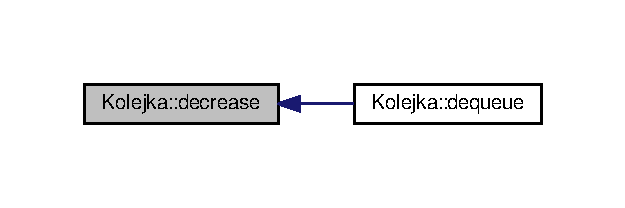
\includegraphics[width=300pt]{class_kolejka_acff09ebfbec69b06c91203bab30d815d_icgraph}
\end{center}
\end{figure}


\hypertarget{class_kolejka_af23261614bcf242a1934a99688a2debc}{\index{Kolejka@{Kolejka}!dequeue@{dequeue}}
\index{dequeue@{dequeue}!Kolejka@{Kolejka}}
\subsubsection[{dequeue}]{\setlength{\rightskip}{0pt plus 5cm}int Kolejka\-::dequeue (
\begin{DoxyParamCaption}
{}
\end{DoxyParamCaption}
)}}\label{class_kolejka_af23261614bcf242a1934a99688a2debc}
\begin{DoxyReturn}{Zwraca}
usuwany element. 
\end{DoxyReturn}


Definicja w linii 69 pliku kolejka.\-cpp.



Oto graf wywołań dla tej funkcji\-:\nopagebreak
\begin{figure}[H]
\begin{center}
\leavevmode
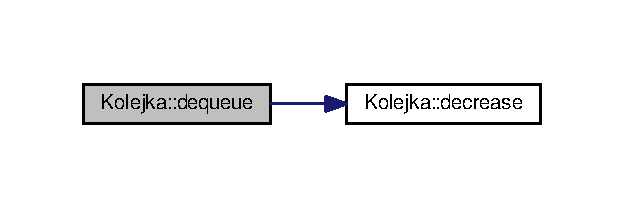
\includegraphics[width=300pt]{class_kolejka_af23261614bcf242a1934a99688a2debc_cgraph}
\end{center}
\end{figure}


\hypertarget{class_kolejka_a8f3b0111e85f517d9eadb8ce996d4471}{\index{Kolejka@{Kolejka}!enqueue@{enqueue}}
\index{enqueue@{enqueue}!Kolejka@{Kolejka}}
\subsubsection[{enqueue}]{\setlength{\rightskip}{0pt plus 5cm}void Kolejka\-::enqueue (
\begin{DoxyParamCaption}
\item[{int}]{\-\_\-elem}
\end{DoxyParamCaption}
)}}\label{class_kolejka_a8f3b0111e85f517d9eadb8ce996d4471}

\begin{DoxyParams}[1]{Parametry}
\mbox{\tt in}  & {\em \-\_\-elem} & -\/ dodawany element. \\
\hline
\end{DoxyParams}


Definicja w linii 60 pliku kolejka.\-cpp.



Oto graf wywołań dla tej funkcji\-:\nopagebreak
\begin{figure}[H]
\begin{center}
\leavevmode
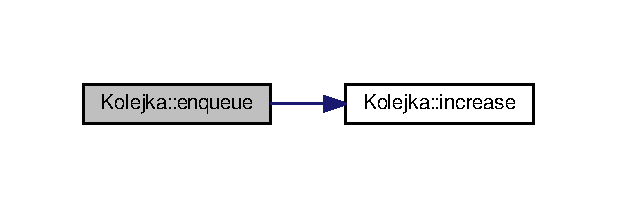
\includegraphics[width=296pt]{class_kolejka_a8f3b0111e85f517d9eadb8ce996d4471_cgraph}
\end{center}
\end{figure}


\hypertarget{class_kolejka_ab4f51f0ec7fef36a85af6cfd1c257427}{\index{Kolejka@{Kolejka}!increase@{increase}}
\index{increase@{increase}!Kolejka@{Kolejka}}
\subsubsection[{increase}]{\setlength{\rightskip}{0pt plus 5cm}void Kolejka\-::increase (
\begin{DoxyParamCaption}
{}
\end{DoxyParamCaption}
)\hspace{0.3cm}{\ttfamily [private]}}}\label{class_kolejka_ab4f51f0ec7fef36a85af6cfd1c257427}


Definicja w linii 33 pliku kolejka.\-cpp.



Oto graf wywoływań tej funkcji\-:\nopagebreak
\begin{figure}[H]
\begin{center}
\leavevmode
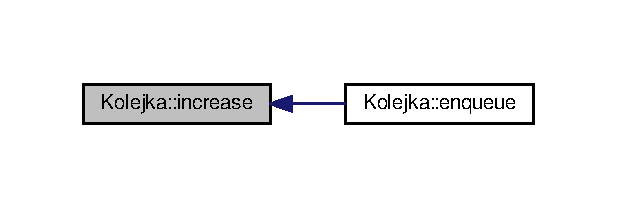
\includegraphics[width=296pt]{class_kolejka_ab4f51f0ec7fef36a85af6cfd1c257427_icgraph}
\end{center}
\end{figure}




Dokumentacja dla tej klasy została wygenerowana z plików\-:\begin{DoxyCompactItemize}
\item 
\hyperlink{kolejka_8hh}{kolejka.\-hh}\item 
\hyperlink{kolejka_8cpp}{kolejka.\-cpp}\end{DoxyCompactItemize}

\hypertarget{struct_komorka}{\section{Dokumentacja struktury Komorka}
\label{struct_komorka}\index{Komorka@{Komorka}}
}


Struktura \hyperlink{struct_komorka}{Komorka}. Obiekt tego typu reprezentuje pojedyncza komorke wraz ze wskaznikiem na nastepna komorke listy.  




{\ttfamily \#include $<$lista.\-hh$>$}



Diagram współpracy dla Komorka\-:\nopagebreak
\begin{figure}[H]
\begin{center}
\leavevmode
\includegraphics[width=174pt]{struct_komorka__coll__graph}
\end{center}
\end{figure}
\subsection*{Metody publiczne}
\begin{DoxyCompactItemize}
\item 
\hyperlink{struct_komorka_a643e9921895597e4d2243cd10b8ee856}{Komorka} (int \-\_\-elem)
\begin{DoxyCompactList}\small\item\em Konstruktor paramteryczny obiektu \hyperlink{struct_komorka}{Komorka}. \end{DoxyCompactList}\item 
\hyperlink{struct_komorka_a6e4b1985b1400b18a0561d8ca7e4768e}{$\sim$\-Komorka} ()
\begin{DoxyCompactList}\small\item\em Destruktor obiektu \hyperlink{struct_komorka}{Komorka}. \end{DoxyCompactList}\end{DoxyCompactItemize}
\subsection*{Atrybuty publiczne}
\begin{DoxyCompactItemize}
\item 
int \hyperlink{struct_komorka_acd355a461762f0e26c785cb66bb604e1}{elem}
\begin{DoxyCompactList}\small\item\em Wartosc elementu w pojedynczej komorce. \end{DoxyCompactList}\item 
\hyperlink{struct_komorka}{Komorka} $\ast$ \hyperlink{struct_komorka_adcee60379726fe686fabcf3addb179c1}{next}
\begin{DoxyCompactList}\small\item\em Wskaznik na nastepna komorke listy. \end{DoxyCompactList}\end{DoxyCompactItemize}


\subsection{Opis szczegółowy}


Definicja w linii 9 pliku lista.\-hh.



\subsection{Dokumentacja konstruktora i destruktora}
\hypertarget{struct_komorka_a643e9921895597e4d2243cd10b8ee856}{\index{Komorka@{Komorka}!Komorka@{Komorka}}
\index{Komorka@{Komorka}!Komorka@{Komorka}}
\subsubsection[{Komorka}]{\setlength{\rightskip}{0pt plus 5cm}Komorka\-::\-Komorka (
\begin{DoxyParamCaption}
\item[{int}]{\-\_\-elem}
\end{DoxyParamCaption}
)}}\label{struct_komorka_a643e9921895597e4d2243cd10b8ee856}

\begin{DoxyParams}[1]{Parametry}
\mbox{\tt in}  & {\em \-\_\-elem} & -\/ wartosc przechowywanego elementu. \\
\hline
\end{DoxyParams}


Definicja w linii 7 pliku lista.\-cpp.

\hypertarget{struct_komorka_a6e4b1985b1400b18a0561d8ca7e4768e}{\index{Komorka@{Komorka}!$\sim$\-Komorka@{$\sim$\-Komorka}}
\index{$\sim$\-Komorka@{$\sim$\-Komorka}!Komorka@{Komorka}}
\subsubsection[{$\sim$\-Komorka}]{\setlength{\rightskip}{0pt plus 5cm}Komorka\-::$\sim$\-Komorka (
\begin{DoxyParamCaption}
{}
\end{DoxyParamCaption}
)\hspace{0.3cm}{\ttfamily [inline]}}}\label{struct_komorka_a6e4b1985b1400b18a0561d8ca7e4768e}


Definicja w linii 26 pliku lista.\-hh.



\subsection{Dokumentacja atrybutów składowych}
\hypertarget{struct_komorka_acd355a461762f0e26c785cb66bb604e1}{\index{Komorka@{Komorka}!elem@{elem}}
\index{elem@{elem}!Komorka@{Komorka}}
\subsubsection[{elem}]{\setlength{\rightskip}{0pt plus 5cm}int Komorka\-::elem}}\label{struct_komorka_acd355a461762f0e26c785cb66bb604e1}


Definicja w linii 13 pliku lista.\-hh.

\hypertarget{struct_komorka_adcee60379726fe686fabcf3addb179c1}{\index{Komorka@{Komorka}!next@{next}}
\index{next@{next}!Komorka@{Komorka}}
\subsubsection[{next}]{\setlength{\rightskip}{0pt plus 5cm}{\bf Komorka}$\ast$ Komorka\-::next}}\label{struct_komorka_adcee60379726fe686fabcf3addb179c1}


Definicja w linii 17 pliku lista.\-hh.



Dokumentacja dla tej struktury została wygenerowana z plików\-:\begin{DoxyCompactItemize}
\item 
\hyperlink{lista_8hh}{lista.\-hh}\item 
\hyperlink{lista_8cpp}{lista.\-cpp}\end{DoxyCompactItemize}

\hypertarget{struct_lista}{\section{Dokumentacja struktury Lista}
\label{struct_lista}\index{Lista@{Lista}}
}


Klasa \hyperlink{struct_lista}{Lista} modelujaca strukture danych typu lista. Obiekt tego typu reprezentuje strukture danych typu lista wraz z operacjami mozliwymi do wykonania na tej strukturze.  




{\ttfamily \#include $<$lista.\-hh$>$}



Diagram współpracy dla Lista\-:
\nopagebreak
\begin{figure}[H]
\begin{center}
\leavevmode
\includegraphics[width=174pt]{struct_lista__coll__graph}
\end{center}
\end{figure}
\subsection*{Metody publiczne}
\begin{DoxyCompactItemize}
\item 
\hyperlink{struct_lista_a1f668b36909182ef1360b48503529a31}{Lista} ()
\begin{DoxyCompactList}\small\item\em Konstruktor obiektu \hyperlink{struct_lista}{Lista}. \end{DoxyCompactList}\item 
\hyperlink{struct_lista_a4d7394b2728a00ad8404965b2e15d096}{$\sim$\-Lista} ()
\begin{DoxyCompactList}\small\item\em Destruktor obiektu \hyperlink{struct_lista}{Lista}. \end{DoxyCompactList}\item 
void \hyperlink{struct_lista_ae3bfec9ea8f7f63172f49500ffa7bf49}{insert\-\_\-last} (int \-\_\-elem)
\begin{DoxyCompactList}\small\item\em Metoda dodawnia elementu. Metoda sluzy do dodawania elementu do konca listy. \end{DoxyCompactList}\item 
int \hyperlink{struct_lista_ad43dc38036e49d500a8ece8c3bf57ee4}{remove\-\_\-front} ()
\begin{DoxyCompactList}\small\item\em Metoda usuwania elementu. Metoda sluzy do usuwania elementu na poczatku listy. \end{DoxyCompactList}\end{DoxyCompactItemize}
\subsection*{Atrybuty prywatne}
\begin{DoxyCompactItemize}
\item 
\hyperlink{struct_komorka}{Komorka} $\ast$ \hyperlink{struct_lista_aeba20505030183d334971bd44c3c8b95}{head}
\begin{DoxyCompactList}\small\item\em Wskaznik na poczatek listy. \end{DoxyCompactList}\item 
\hyperlink{struct_komorka}{Komorka} $\ast$ \hyperlink{struct_lista_a7d42e5f99e945d97c29d6f764f71f4e7}{tail}
\begin{DoxyCompactList}\small\item\em Wskaznik na koniec listy. \end{DoxyCompactList}\end{DoxyCompactItemize}


\subsection{Opis szczegółowy}


Definicja w linii 34 pliku lista.\-hh.



\subsection{Dokumentacja konstruktora i destruktora}
\hypertarget{struct_lista_a1f668b36909182ef1360b48503529a31}{\index{Lista@{Lista}!Lista@{Lista}}
\index{Lista@{Lista}!Lista@{Lista}}
\subsubsection[{Lista}]{\setlength{\rightskip}{0pt plus 5cm}Lista\-::\-Lista (
\begin{DoxyParamCaption}
{}
\end{DoxyParamCaption}
)\hspace{0.3cm}{\ttfamily [inline]}}}\label{struct_lista_a1f668b36909182ef1360b48503529a31}


Definicja w linii 49 pliku lista.\-hh.

\hypertarget{struct_lista_a4d7394b2728a00ad8404965b2e15d096}{\index{Lista@{Lista}!$\sim$\-Lista@{$\sim$\-Lista}}
\index{$\sim$\-Lista@{$\sim$\-Lista}!Lista@{Lista}}
\subsubsection[{$\sim$\-Lista}]{\setlength{\rightskip}{0pt plus 5cm}Lista\-::$\sim$\-Lista (
\begin{DoxyParamCaption}
{}
\end{DoxyParamCaption}
)\hspace{0.3cm}{\ttfamily [inline]}}}\label{struct_lista_a4d7394b2728a00ad8404965b2e15d096}


Definicja w linii 53 pliku lista.\-hh.



\subsection{Dokumentacja funkcji składowych}
\hypertarget{struct_lista_ae3bfec9ea8f7f63172f49500ffa7bf49}{\index{Lista@{Lista}!insert\-\_\-last@{insert\-\_\-last}}
\index{insert\-\_\-last@{insert\-\_\-last}!Lista@{Lista}}
\subsubsection[{insert\-\_\-last}]{\setlength{\rightskip}{0pt plus 5cm}void Lista\-::insert\-\_\-last (
\begin{DoxyParamCaption}
\item[{int}]{\-\_\-elem}
\end{DoxyParamCaption}
)}}\label{struct_lista_ae3bfec9ea8f7f63172f49500ffa7bf49}

\begin{DoxyParams}[1]{Parametry}
\mbox{\tt in}  & {\em \-\_\-elem} & -\/ dodawany element. \\
\hline
\end{DoxyParams}


Definicja w linii 14 pliku lista.\-cpp.

\hypertarget{struct_lista_ad43dc38036e49d500a8ece8c3bf57ee4}{\index{Lista@{Lista}!remove\-\_\-front@{remove\-\_\-front}}
\index{remove\-\_\-front@{remove\-\_\-front}!Lista@{Lista}}
\subsubsection[{remove\-\_\-front}]{\setlength{\rightskip}{0pt plus 5cm}int Lista\-::remove\-\_\-front (
\begin{DoxyParamCaption}
{}
\end{DoxyParamCaption}
)}}\label{struct_lista_ad43dc38036e49d500a8ece8c3bf57ee4}
\begin{DoxyReturn}{Zwraca}
usuwany element. 
\end{DoxyReturn}


Definicja w linii 29 pliku lista.\-cpp.



\subsection{Dokumentacja atrybutów składowych}
\hypertarget{struct_lista_aeba20505030183d334971bd44c3c8b95}{\index{Lista@{Lista}!head@{head}}
\index{head@{head}!Lista@{Lista}}
\subsubsection[{head}]{\setlength{\rightskip}{0pt plus 5cm}{\bf Komorka}$\ast$ Lista\-::head\hspace{0.3cm}{\ttfamily [private]}}}\label{struct_lista_aeba20505030183d334971bd44c3c8b95}


Definicja w linii 39 pliku lista.\-hh.

\hypertarget{struct_lista_a7d42e5f99e945d97c29d6f764f71f4e7}{\index{Lista@{Lista}!tail@{tail}}
\index{tail@{tail}!Lista@{Lista}}
\subsubsection[{tail}]{\setlength{\rightskip}{0pt plus 5cm}{\bf Komorka}$\ast$ Lista\-::tail\hspace{0.3cm}{\ttfamily [private]}}}\label{struct_lista_a7d42e5f99e945d97c29d6f764f71f4e7}


Definicja w linii 43 pliku lista.\-hh.



Dokumentacja dla tej struktury została wygenerowana z plików\-:\begin{DoxyCompactItemize}
\item 
\hyperlink{lista_8hh}{lista.\-hh}\item 
\hyperlink{lista_8cpp}{lista.\-cpp}\end{DoxyCompactItemize}

\hypertarget{class_mieszajaca}{\section{Dokumentacja klasy Mieszajaca}
\label{class_mieszajaca}\index{Mieszajaca@{Mieszajaca}}
}


Klasa \hyperlink{class_mieszajaca}{Mieszajaca}. Obiekt tego typu reprezentuje pojedyncza strukture danych typu tablica mieszajaca wraz z operacjami mozliwymi do wykonania na tej strukturze.  




{\ttfamily \#include $<$mieszajaca.\-hh$>$}



Diagram współpracy dla Mieszajaca\-:
\nopagebreak
\begin{figure}[H]
\begin{center}
\leavevmode
\includegraphics[width=144pt]{class_mieszajaca__coll__graph}
\end{center}
\end{figure}
\subsection*{Metody publiczne}
\begin{DoxyCompactItemize}
\item 
\hyperlink{class_mieszajaca_ab500c9ba068fbe15f9aa05d83df500ed}{Mieszajaca} ()
\begin{DoxyCompactList}\small\item\em Konstruktor obiektu \hyperlink{class_mieszajaca}{Mieszajaca}. \end{DoxyCompactList}\item 
\hyperlink{class_mieszajaca_a057f62fac3404b4748b4b38dbfc25cc2}{Mieszajaca} (long \-\_\-size)
\begin{DoxyCompactList}\small\item\em Konstruktor parametryczny obiektu mieszajaca. \end{DoxyCompactList}\item 
\hyperlink{class_mieszajaca_a66a712ce4807c9330ae36f6561101a57}{$\sim$\-Mieszajaca} ()
\begin{DoxyCompactList}\small\item\em Destruktor obiektu \hyperlink{class_mieszajaca}{Mieszajaca}. \end{DoxyCompactList}\item 
int \& \hyperlink{class_mieszajaca_ad2a90e2facd4df39cd1efe8a75ce60a4}{operator\mbox{[}$\,$\mbox{]}} (const char $\ast$key)
\begin{DoxyCompactList}\small\item\em Przeladowanie operatora nawiasu kwadratowego. Sluzy do wpisywania klucza oraz wartosci. \end{DoxyCompactList}\end{DoxyCompactItemize}
\subsection*{Metody chronione}
\begin{DoxyCompactItemize}
\item 
unsigned \hyperlink{class_mieszajaca_a4508ea747690242d296d5095ccd6e2ec}{sax\-\_\-hash} (const char $\ast$key) const 
\begin{DoxyCompactList}\small\item\em Funkcja haszująca Shift-\/\-Add-\/\-X\-O\-R. \end{DoxyCompactList}\item 
unsigned \hyperlink{class_mieszajaca_a5367ffb855dcf48ed51deaab30896249}{fnv\-\_\-hash} (const char $\ast$key) const 
\begin{DoxyCompactList}\small\item\em Funkcja haszująca Fovler/\-Voll/\-No. \end{DoxyCompactList}\item 
\hyperlink{struct_m_node}{M\-Node} $\ast$ \hyperlink{class_mieszajaca_aade3fc649e04b21a9497d8d3b6939082}{find} (const char $\ast$key) const 
\begin{DoxyCompactList}\small\item\em Metoda wyszukiwania elementu o podanym kluczu. \end{DoxyCompactList}\item 
void \hyperlink{class_mieszajaca_a6c58c6edcfac89082e7d49538c8e5c74}{insert} (const char $\ast$key, int value)
\begin{DoxyCompactList}\small\item\em Metoda wstawiania nowej pary klucz-\/wartosc. \end{DoxyCompactList}\end{DoxyCompactItemize}
\subsection*{Atrybuty prywatne}
\begin{DoxyCompactItemize}
\item 
\hyperlink{struct_m_node}{M\-Node} $\ast$$\ast$ \hyperlink{class_mieszajaca_adb0f4884ed63b184cf0bd63e757490cd}{tab\-\_\-l}
\begin{DoxyCompactList}\small\item\em Wskaznik na lewa tablice elementow. \end{DoxyCompactList}\item 
\hyperlink{struct_m_node}{M\-Node} $\ast$$\ast$ \hyperlink{class_mieszajaca_a37e86d776d7eeef64b36f04e91b44a4c}{tab\-\_\-p}
\begin{DoxyCompactList}\small\item\em Wskaznik na lewa tablice elementow. \end{DoxyCompactList}\item 
long \hyperlink{class_mieszajaca_a6521d97bf16d4fd92d147aafd2a56e3f}{size}
\begin{DoxyCompactList}\small\item\em Rozmiar tablic. \end{DoxyCompactList}\end{DoxyCompactItemize}
\subsection*{Przyjaciele}
\begin{DoxyCompactItemize}
\item 
std\-::ostream \& \hyperlink{class_mieszajaca_a6c4fd68588109e2cca8a88cee92b9a67}{operator$<$$<$} (std\-::ostream \&stream, \hyperlink{class_mieszajaca}{Mieszajaca} \&l)
\begin{DoxyCompactList}\small\item\em Przeladowanie operatora przesuniecia bitowego. Sluzy do wypisywania zawartosci tablicy mieszajacej na strumien wyjsciowy. \end{DoxyCompactList}\end{DoxyCompactItemize}


\subsection{Opis szczegółowy}


Definicja w linii 74 pliku mieszajaca.\-hh.



\subsection{Dokumentacja konstruktora i destruktora}
\hypertarget{class_mieszajaca_ab500c9ba068fbe15f9aa05d83df500ed}{\index{Mieszajaca@{Mieszajaca}!Mieszajaca@{Mieszajaca}}
\index{Mieszajaca@{Mieszajaca}!Mieszajaca@{Mieszajaca}}
\subsubsection[{Mieszajaca}]{\setlength{\rightskip}{0pt plus 5cm}Mieszajaca\-::\-Mieszajaca (
\begin{DoxyParamCaption}
{}
\end{DoxyParamCaption}
)}}\label{class_mieszajaca_ab500c9ba068fbe15f9aa05d83df500ed}


Definicja w linii 7 pliku mieszajaca.\-cpp.

\hypertarget{class_mieszajaca_a057f62fac3404b4748b4b38dbfc25cc2}{\index{Mieszajaca@{Mieszajaca}!Mieszajaca@{Mieszajaca}}
\index{Mieszajaca@{Mieszajaca}!Mieszajaca@{Mieszajaca}}
\subsubsection[{Mieszajaca}]{\setlength{\rightskip}{0pt plus 5cm}Mieszajaca\-::\-Mieszajaca (
\begin{DoxyParamCaption}
\item[{long}]{\-\_\-size}
\end{DoxyParamCaption}
)}}\label{class_mieszajaca_a057f62fac3404b4748b4b38dbfc25cc2}

\begin{DoxyParams}[1]{Parametry}
\mbox{\tt in}  & {\em \-\_\-size} & -\/ rozmiar tworzonej tablicy mieszajacej. \\
\hline
\end{DoxyParams}


Definicja w linii 19 pliku mieszajaca.\-cpp.

\hypertarget{class_mieszajaca_a66a712ce4807c9330ae36f6561101a57}{\index{Mieszajaca@{Mieszajaca}!$\sim$\-Mieszajaca@{$\sim$\-Mieszajaca}}
\index{$\sim$\-Mieszajaca@{$\sim$\-Mieszajaca}!Mieszajaca@{Mieszajaca}}
\subsubsection[{$\sim$\-Mieszajaca}]{\setlength{\rightskip}{0pt plus 5cm}Mieszajaca\-::$\sim$\-Mieszajaca (
\begin{DoxyParamCaption}
{}
\end{DoxyParamCaption}
)}}\label{class_mieszajaca_a66a712ce4807c9330ae36f6561101a57}


Definicja w linii 31 pliku mieszajaca.\-cpp.



\subsection{Dokumentacja funkcji składowych}
\hypertarget{class_mieszajaca_aade3fc649e04b21a9497d8d3b6939082}{\index{Mieszajaca@{Mieszajaca}!find@{find}}
\index{find@{find}!Mieszajaca@{Mieszajaca}}
\subsubsection[{find}]{\setlength{\rightskip}{0pt plus 5cm}{\bf M\-Node} $\ast$ Mieszajaca\-::find (
\begin{DoxyParamCaption}
\item[{const char $\ast$}]{key}
\end{DoxyParamCaption}
) const\hspace{0.3cm}{\ttfamily [protected]}}}\label{class_mieszajaca_aade3fc649e04b21a9497d8d3b6939082}

\begin{DoxyParams}[1]{Parametry}
\mbox{\tt in}  & {\em key} & -\/ wskaznik na wyszukiwany klucz. \\
\hline
\end{DoxyParams}
\begin{DoxyReturn}{Zwraca}
wskaznik na szukana pare klucz-\/wartosc, nullprt gdy nie znalezniono klucza. 
\end{DoxyReturn}


Definicja w linii 90 pliku mieszajaca.\-cpp.



Oto graf wywołań dla tej funkcji\-:
\nopagebreak
\begin{figure}[H]
\begin{center}
\leavevmode
\includegraphics[width=314pt]{class_mieszajaca_aade3fc649e04b21a9497d8d3b6939082_cgraph}
\end{center}
\end{figure}




Oto graf wywoływań tej funkcji\-:
\nopagebreak
\begin{figure}[H]
\begin{center}
\leavevmode
\includegraphics[width=314pt]{class_mieszajaca_aade3fc649e04b21a9497d8d3b6939082_icgraph}
\end{center}
\end{figure}


\hypertarget{class_mieszajaca_a5367ffb855dcf48ed51deaab30896249}{\index{Mieszajaca@{Mieszajaca}!fnv\-\_\-hash@{fnv\-\_\-hash}}
\index{fnv\-\_\-hash@{fnv\-\_\-hash}!Mieszajaca@{Mieszajaca}}
\subsubsection[{fnv\-\_\-hash}]{\setlength{\rightskip}{0pt plus 5cm}unsigned Mieszajaca\-::fnv\-\_\-hash (
\begin{DoxyParamCaption}
\item[{const char $\ast$}]{key}
\end{DoxyParamCaption}
) const\hspace{0.3cm}{\ttfamily [protected]}}}\label{class_mieszajaca_a5367ffb855dcf48ed51deaab30896249}

\begin{DoxyParams}[1]{Parametry}
\mbox{\tt in}  & {\em key} & -\/ wskaznik na wyszukiwany klucz. \\
\hline
\end{DoxyParams}
\begin{DoxyReturn}{Zwraca}
indeks. 
\end{DoxyReturn}


Definicja w linii 55 pliku mieszajaca.\-cpp.



Oto graf wywoływań tej funkcji\-:
\nopagebreak
\begin{figure}[H]
\begin{center}
\leavevmode
\includegraphics[width=350pt]{class_mieszajaca_a5367ffb855dcf48ed51deaab30896249_icgraph}
\end{center}
\end{figure}


\hypertarget{class_mieszajaca_a6c58c6edcfac89082e7d49538c8e5c74}{\index{Mieszajaca@{Mieszajaca}!insert@{insert}}
\index{insert@{insert}!Mieszajaca@{Mieszajaca}}
\subsubsection[{insert}]{\setlength{\rightskip}{0pt plus 5cm}void Mieszajaca\-::insert (
\begin{DoxyParamCaption}
\item[{const char $\ast$}]{key, }
\item[{int}]{value}
\end{DoxyParamCaption}
)\hspace{0.3cm}{\ttfamily [protected]}}}\label{class_mieszajaca_a6c58c6edcfac89082e7d49538c8e5c74}

\begin{DoxyParams}[1]{Parametry}
\mbox{\tt in}  & {\em key} & -\/ wskaznik na klucz. \\
\hline
\mbox{\tt in}  & {\em value} & -\/ wartosc klucza. \\
\hline
\end{DoxyParams}


Definicja w linii 71 pliku mieszajaca.\-cpp.



Oto graf wywołań dla tej funkcji\-:
\nopagebreak
\begin{figure}[H]
\begin{center}
\leavevmode
\includegraphics[width=322pt]{class_mieszajaca_a6c58c6edcfac89082e7d49538c8e5c74_cgraph}
\end{center}
\end{figure}




Oto graf wywoływań tej funkcji\-:
\nopagebreak
\begin{figure}[H]
\begin{center}
\leavevmode
\includegraphics[width=322pt]{class_mieszajaca_a6c58c6edcfac89082e7d49538c8e5c74_icgraph}
\end{center}
\end{figure}


\hypertarget{class_mieszajaca_ad2a90e2facd4df39cd1efe8a75ce60a4}{\index{Mieszajaca@{Mieszajaca}!operator\mbox{[}$\,$\mbox{]}@{operator[]}}
\index{operator\mbox{[}$\,$\mbox{]}@{operator[]}!Mieszajaca@{Mieszajaca}}
\subsubsection[{operator[]}]{\setlength{\rightskip}{0pt plus 5cm}int \& Mieszajaca\-::operator\mbox{[}$\,$\mbox{]} (
\begin{DoxyParamCaption}
\item[{const char $\ast$}]{key}
\end{DoxyParamCaption}
)}}\label{class_mieszajaca_ad2a90e2facd4df39cd1efe8a75ce60a4}

\begin{DoxyParams}[1]{Parametry}
\mbox{\tt in}  & {\em key} & -\/ wskaznik na klucz. \\
\hline
\end{DoxyParams}
\begin{DoxyReturn}{Zwraca}
wartosc klucza. 
\end{DoxyReturn}


Definicja w linii 108 pliku mieszajaca.\-cpp.



Oto graf wywołań dla tej funkcji\-:
\nopagebreak
\begin{figure}[H]
\begin{center}
\leavevmode
\includegraphics[width=350pt]{class_mieszajaca_ad2a90e2facd4df39cd1efe8a75ce60a4_cgraph}
\end{center}
\end{figure}


\hypertarget{class_mieszajaca_a4508ea747690242d296d5095ccd6e2ec}{\index{Mieszajaca@{Mieszajaca}!sax\-\_\-hash@{sax\-\_\-hash}}
\index{sax\-\_\-hash@{sax\-\_\-hash}!Mieszajaca@{Mieszajaca}}
\subsubsection[{sax\-\_\-hash}]{\setlength{\rightskip}{0pt plus 5cm}unsigned Mieszajaca\-::sax\-\_\-hash (
\begin{DoxyParamCaption}
\item[{const char $\ast$}]{key}
\end{DoxyParamCaption}
) const\hspace{0.3cm}{\ttfamily [protected]}}}\label{class_mieszajaca_a4508ea747690242d296d5095ccd6e2ec}

\begin{DoxyParams}[1]{Parametry}
\mbox{\tt in}  & {\em key} & -\/ wskaznik na wyszukiwany klucz. \\
\hline
\end{DoxyParams}
\begin{DoxyReturn}{Zwraca}
indeks. 
\end{DoxyReturn}


Definicja w linii 38 pliku mieszajaca.\-cpp.



Oto graf wywoływań tej funkcji\-:
\nopagebreak
\begin{figure}[H]
\begin{center}
\leavevmode
\includegraphics[width=350pt]{class_mieszajaca_a4508ea747690242d296d5095ccd6e2ec_icgraph}
\end{center}
\end{figure}




\subsection{Dokumentacja przyjaciół i funkcji związanych}
\hypertarget{class_mieszajaca_a6c4fd68588109e2cca8a88cee92b9a67}{\index{Mieszajaca@{Mieszajaca}!operator$<$$<$@{operator$<$$<$}}
\index{operator$<$$<$@{operator$<$$<$}!Mieszajaca@{Mieszajaca}}
\subsubsection[{operator$<$$<$}]{\setlength{\rightskip}{0pt plus 5cm}std\-::ostream\& operator$<$$<$ (
\begin{DoxyParamCaption}
\item[{std\-::ostream \&}]{stream, }
\item[{{\bf Mieszajaca} \&}]{l}
\end{DoxyParamCaption}
)\hspace{0.3cm}{\ttfamily [friend]}}}\label{class_mieszajaca_a6c4fd68588109e2cca8a88cee92b9a67}

\begin{DoxyParams}[1]{Parametry}
\mbox{\tt in}  & {\em stream} & -\/ referencja do strumienia wyjsciowego. \\
\hline
\mbox{\tt in}  & {\em l} & -\/ referencja do tablicy. \\
\hline
\end{DoxyParams}
\begin{DoxyReturn}{Zwraca}
strumien wyjsciowy. 
\end{DoxyReturn}


Definicja w linii 147 pliku mieszajaca.\-hh.



\subsection{Dokumentacja atrybutów składowych}
\hypertarget{class_mieszajaca_a6521d97bf16d4fd92d147aafd2a56e3f}{\index{Mieszajaca@{Mieszajaca}!size@{size}}
\index{size@{size}!Mieszajaca@{Mieszajaca}}
\subsubsection[{size}]{\setlength{\rightskip}{0pt plus 5cm}long Mieszajaca\-::size\hspace{0.3cm}{\ttfamily [private]}}}\label{class_mieszajaca_a6521d97bf16d4fd92d147aafd2a56e3f}


Definicja w linii 87 pliku mieszajaca.\-hh.

\hypertarget{class_mieszajaca_adb0f4884ed63b184cf0bd63e757490cd}{\index{Mieszajaca@{Mieszajaca}!tab\-\_\-l@{tab\-\_\-l}}
\index{tab\-\_\-l@{tab\-\_\-l}!Mieszajaca@{Mieszajaca}}
\subsubsection[{tab\-\_\-l}]{\setlength{\rightskip}{0pt plus 5cm}{\bf M\-Node}$\ast$$\ast$ Mieszajaca\-::tab\-\_\-l\hspace{0.3cm}{\ttfamily [private]}}}\label{class_mieszajaca_adb0f4884ed63b184cf0bd63e757490cd}


Definicja w linii 79 pliku mieszajaca.\-hh.

\hypertarget{class_mieszajaca_a37e86d776d7eeef64b36f04e91b44a4c}{\index{Mieszajaca@{Mieszajaca}!tab\-\_\-p@{tab\-\_\-p}}
\index{tab\-\_\-p@{tab\-\_\-p}!Mieszajaca@{Mieszajaca}}
\subsubsection[{tab\-\_\-p}]{\setlength{\rightskip}{0pt plus 5cm}{\bf M\-Node}$\ast$$\ast$ Mieszajaca\-::tab\-\_\-p\hspace{0.3cm}{\ttfamily [private]}}}\label{class_mieszajaca_a37e86d776d7eeef64b36f04e91b44a4c}


Definicja w linii 83 pliku mieszajaca.\-hh.



Dokumentacja dla tej klasy została wygenerowana z plików\-:\begin{DoxyCompactItemize}
\item 
\hyperlink{mieszajaca_8hh}{mieszajaca.\-hh}\item 
\hyperlink{mieszajaca_8cpp}{mieszajaca.\-cpp}\end{DoxyCompactItemize}

\hypertarget{struct_m_node}{\section{Dokumentacja struktury M\-Node}
\label{struct_m_node}\index{M\-Node@{M\-Node}}
}


Struktura \hyperlink{struct_a_node}{A\-Node}. Obiekt tego typu reprezentuje pojedyncza komorke tablicy mieszajacej;.  




{\ttfamily \#include $<$mieszajaca.\-hh$>$}

\subsection*{Metody publiczne}
\begin{DoxyCompactItemize}
\item 
\hyperlink{struct_m_node_a4f5e9c524bf97b5694d8f008e9436996}{M\-Node} ()
\item 
\hyperlink{struct_m_node_a579e99923a2f7cdacc468d2df179f9c3}{M\-Node} (const char $\ast$k)
\begin{DoxyCompactList}\small\item\em Konstruktor paramteryczny struktury \hyperlink{struct_m_node}{M\-Node}. \end{DoxyCompactList}\item 
\hyperlink{struct_m_node_a9fc5ae595ed230ab6af613daf0363303}{M\-Node} (const \hyperlink{struct_m_node}{M\-Node} \&s)
\begin{DoxyCompactList}\small\item\em Konstruktor paramteryczny struktury \hyperlink{struct_m_node}{M\-Node}. \end{DoxyCompactList}\item 
\hyperlink{struct_m_node_aa96f44f28eee1e25a9a267baaa61813d}{$\sim$\-M\-Node} ()
\begin{DoxyCompactList}\small\item\em Destruktor struktury node. \end{DoxyCompactList}\end{DoxyCompactItemize}
\subsection*{Atrybuty publiczne}
\begin{DoxyCompactItemize}
\item 
char $\ast$ \hyperlink{struct_m_node_a34eaceeae213bc93c9f18b752801a1f0}{key}
\begin{DoxyCompactList}\small\item\em Wskaznik na klucz. \end{DoxyCompactList}\item 
int \hyperlink{struct_m_node_a9ba04f597c758c10b9f2309322fe4c8d}{val}
\begin{DoxyCompactList}\small\item\em Wartosc klucza. \end{DoxyCompactList}\end{DoxyCompactItemize}
\subsection*{Metody prywatne}
\begin{DoxyCompactItemize}
\item 
\hyperlink{struct_m_node}{M\-Node} \& \hyperlink{struct_m_node_a6b2f4245f982546c8437f599bcf410b1}{operator=} (const \hyperlink{struct_m_node}{M\-Node} \&)
\begin{DoxyCompactList}\small\item\em Przeladowanie operatora przypisania. Zabezpieczenie przed automatycznym operatorem przypisania. \end{DoxyCompactList}\end{DoxyCompactItemize}


\subsection{Opis szczegółowy}


Definicja w linii 11 pliku mieszajaca.\-hh.



\subsection{Dokumentacja konstruktora i destruktora}
\hypertarget{struct_m_node_a4f5e9c524bf97b5694d8f008e9436996}{\index{M\-Node@{M\-Node}!M\-Node@{M\-Node}}
\index{M\-Node@{M\-Node}!MNode@{M\-Node}}
\subsubsection[{M\-Node}]{\setlength{\rightskip}{0pt plus 5cm}M\-Node\-::\-M\-Node (
\begin{DoxyParamCaption}
{}
\end{DoxyParamCaption}
)\hspace{0.3cm}{\ttfamily [inline]}}}\label{struct_m_node_a4f5e9c524bf97b5694d8f008e9436996}


Definicja w linii 21 pliku mieszajaca.\-hh.

\hypertarget{struct_m_node_a579e99923a2f7cdacc468d2df179f9c3}{\index{M\-Node@{M\-Node}!M\-Node@{M\-Node}}
\index{M\-Node@{M\-Node}!MNode@{M\-Node}}
\subsubsection[{M\-Node}]{\setlength{\rightskip}{0pt plus 5cm}M\-Node\-::\-M\-Node (
\begin{DoxyParamCaption}
\item[{const char $\ast$}]{k}
\end{DoxyParamCaption}
)\hspace{0.3cm}{\ttfamily [inline]}}}\label{struct_m_node_a579e99923a2f7cdacc468d2df179f9c3}

\begin{DoxyParams}[1]{Parametry}
\mbox{\tt in}  & {\em k} & -\/ wskaznik na klucz. \\
\hline
\end{DoxyParams}


Definicja w linii 30 pliku mieszajaca.\-hh.

\hypertarget{struct_m_node_a9fc5ae595ed230ab6af613daf0363303}{\index{M\-Node@{M\-Node}!M\-Node@{M\-Node}}
\index{M\-Node@{M\-Node}!MNode@{M\-Node}}
\subsubsection[{M\-Node}]{\setlength{\rightskip}{0pt plus 5cm}M\-Node\-::\-M\-Node (
\begin{DoxyParamCaption}
\item[{const {\bf M\-Node} \&}]{s}
\end{DoxyParamCaption}
)\hspace{0.3cm}{\ttfamily [inline]}}}\label{struct_m_node_a9fc5ae595ed230ab6af613daf0363303}

\begin{DoxyParams}[1]{Parametry}
\mbox{\tt in}  & {\em s} & -\/ referencja do pary klucz-\/wartosc. \\
\hline
\end{DoxyParams}


Definicja w linii 39 pliku mieszajaca.\-hh.

\hypertarget{struct_m_node_aa96f44f28eee1e25a9a267baaa61813d}{\index{M\-Node@{M\-Node}!$\sim$\-M\-Node@{$\sim$\-M\-Node}}
\index{$\sim$\-M\-Node@{$\sim$\-M\-Node}!MNode@{M\-Node}}
\subsubsection[{$\sim$\-M\-Node}]{\setlength{\rightskip}{0pt plus 5cm}M\-Node\-::$\sim$\-M\-Node (
\begin{DoxyParamCaption}
{}
\end{DoxyParamCaption}
)\hspace{0.3cm}{\ttfamily [inline]}}}\label{struct_m_node_aa96f44f28eee1e25a9a267baaa61813d}


Definicja w linii 54 pliku mieszajaca.\-hh.



\subsection{Dokumentacja funkcji składowych}
\hypertarget{struct_m_node_a6b2f4245f982546c8437f599bcf410b1}{\index{M\-Node@{M\-Node}!operator=@{operator=}}
\index{operator=@{operator=}!MNode@{M\-Node}}
\subsubsection[{operator=}]{\setlength{\rightskip}{0pt plus 5cm}{\bf M\-Node}\& M\-Node\-::operator= (
\begin{DoxyParamCaption}
\item[{const {\bf M\-Node} \&}]{}
\end{DoxyParamCaption}
)\hspace{0.3cm}{\ttfamily [private]}}}\label{struct_m_node_a6b2f4245f982546c8437f599bcf410b1}


\subsection{Dokumentacja atrybutów składowych}
\hypertarget{struct_m_node_a34eaceeae213bc93c9f18b752801a1f0}{\index{M\-Node@{M\-Node}!key@{key}}
\index{key@{key}!MNode@{M\-Node}}
\subsubsection[{key}]{\setlength{\rightskip}{0pt plus 5cm}char$\ast$ M\-Node\-::key}}\label{struct_m_node_a34eaceeae213bc93c9f18b752801a1f0}


Definicja w linii 15 pliku mieszajaca.\-hh.

\hypertarget{struct_m_node_a9ba04f597c758c10b9f2309322fe4c8d}{\index{M\-Node@{M\-Node}!val@{val}}
\index{val@{val}!MNode@{M\-Node}}
\subsubsection[{val}]{\setlength{\rightskip}{0pt plus 5cm}int M\-Node\-::val}}\label{struct_m_node_a9ba04f597c758c10b9f2309322fe4c8d}


Definicja w linii 19 pliku mieszajaca.\-hh.



Dokumentacja dla tej struktury została wygenerowana z pliku\-:\begin{DoxyCompactItemize}
\item 
\hyperlink{mieszajaca_8hh}{mieszajaca.\-hh}\end{DoxyCompactItemize}

\hypertarget{class_observer}{\section{Dokumentacja klasy Observer}
\label{class_observer}\index{Observer@{Observer}}
}


Klasa \hyperlink{class_observer}{Observer} modelujaca obserwatora. Jest to klasa modelujaca ogolnego obserwatora. Przeznaczona jedynie do dziedziczenia.  




{\ttfamily \#include $<$observer.\-hh$>$}



Diagram dziedziczenia dla Observer
\nopagebreak
\begin{figure}[H]
\begin{center}
\leavevmode
\includegraphics[width=166pt]{class_observer__inherit__graph}
\end{center}
\end{figure}
\subsection*{Metody publiczne}
\begin{DoxyCompactItemize}
\item 
int \hyperlink{class_observer_a46f35957f410c0390ccfd03440b5b558}{tell\-\_\-id} ()
\begin{DoxyCompactList}\small\item\em Metoda identyfikacji obserwatora. Sluzy do informowania o identyfikatorze obserwatora. \end{DoxyCompactList}\item 
virtual void \hyperlink{class_observer_ac75e4b339faeb3ea6fe0a01bf0b4a215}{update} ()=0
\begin{DoxyCompactList}\small\item\em Metoda aktualizujaca stan obserwatora. W klasie \hyperlink{class_observer}{Observer} nie ma konkretnego dzialania. \end{DoxyCompactList}\end{DoxyCompactItemize}
\subsection*{Atrybuty chronione}
\begin{DoxyCompactItemize}
\item 
int \hyperlink{class_observer_ac67c499a5b16953f268840890fd7e6ab}{id}
\begin{DoxyCompactList}\small\item\em Identyfikator obserwatora. \end{DoxyCompactList}\item 
unsigned int \hyperlink{class_observer_a6e82806d2c300975d1e194798af109d2}{state\-\_\-id} = 0
\begin{DoxyCompactList}\small\item\em Zmienna zliczajaca aktualizacje. Sluzy do przechowywania informacji o wykonanych aktualizacjach obserwatora. \end{DoxyCompactList}\end{DoxyCompactItemize}


\subsection{Opis szczegółowy}


Definicja w linii 9 pliku observer.\-hh.



\subsection{Dokumentacja funkcji składowych}
\hypertarget{class_observer_a46f35957f410c0390ccfd03440b5b558}{\index{Observer@{Observer}!tell\-\_\-id@{tell\-\_\-id}}
\index{tell\-\_\-id@{tell\-\_\-id}!Observer@{Observer}}
\subsubsection[{tell\-\_\-id}]{\setlength{\rightskip}{0pt plus 5cm}int Observer\-::tell\-\_\-id (
\begin{DoxyParamCaption}
{}
\end{DoxyParamCaption}
)}}\label{class_observer_a46f35957f410c0390ccfd03440b5b558}
\begin{DoxyReturn}{Zwraca}
identyfikator obserwatora. 
\end{DoxyReturn}


Definicja w linii 4 pliku observer.\-cpp.



Oto graf wywoływań tej funkcji\-:
\nopagebreak
\begin{figure}[H]
\begin{center}
\leavevmode
\includegraphics[width=322pt]{class_observer_a46f35957f410c0390ccfd03440b5b558_icgraph}
\end{center}
\end{figure}


\hypertarget{class_observer_ac75e4b339faeb3ea6fe0a01bf0b4a215}{\index{Observer@{Observer}!update@{update}}
\index{update@{update}!Observer@{Observer}}
\subsubsection[{update}]{\setlength{\rightskip}{0pt plus 5cm}virtual void Observer\-::update (
\begin{DoxyParamCaption}
{}
\end{DoxyParamCaption}
)\hspace{0.3cm}{\ttfamily [pure virtual]}}}\label{class_observer_ac75e4b339faeb3ea6fe0a01bf0b4a215}


Implementowany w \hyperlink{class_writing_observer_a7b5aa3fa85ae0e1d27ccd8b08366f043}{Writing\-Observer}.



\subsection{Dokumentacja atrybutów składowych}
\hypertarget{class_observer_ac67c499a5b16953f268840890fd7e6ab}{\index{Observer@{Observer}!id@{id}}
\index{id@{id}!Observer@{Observer}}
\subsubsection[{id}]{\setlength{\rightskip}{0pt plus 5cm}int Observer\-::id\hspace{0.3cm}{\ttfamily [protected]}}}\label{class_observer_ac67c499a5b16953f268840890fd7e6ab}


Definicja w linii 14 pliku observer.\-hh.

\hypertarget{class_observer_a6e82806d2c300975d1e194798af109d2}{\index{Observer@{Observer}!state\-\_\-id@{state\-\_\-id}}
\index{state\-\_\-id@{state\-\_\-id}!Observer@{Observer}}
\subsubsection[{state\-\_\-id}]{\setlength{\rightskip}{0pt plus 5cm}unsigned int Observer\-::state\-\_\-id = 0\hspace{0.3cm}{\ttfamily [protected]}}}\label{class_observer_a6e82806d2c300975d1e194798af109d2}


Definicja w linii 20 pliku observer.\-hh.



Dokumentacja dla tej klasy została wygenerowana z plików\-:\begin{DoxyCompactItemize}
\item 
\hyperlink{observer_8hh}{observer.\-hh}\item 
\hyperlink{observer_8cpp}{observer.\-cpp}\end{DoxyCompactItemize}

\hypertarget{struct_r_b_node}{\section{Dokumentacja struktury R\-B\-Node}
\label{struct_r_b_node}\index{R\-B\-Node@{R\-B\-Node}}
}


{\ttfamily \#include $<$rb\-\_\-tree.\-hh$>$}



Diagram współpracy dla R\-B\-Node\-:\nopagebreak
\begin{figure}[H]
\begin{center}
\leavevmode
\includegraphics[width=172pt]{struct_r_b_node__coll__graph}
\end{center}
\end{figure}
\subsection*{Metody publiczne}
\begin{DoxyCompactItemize}
\item 
\hyperlink{struct_r_b_node_a6c581adb50310ce3794f2e4613ac166c}{R\-B\-Node} ()
\item 
\hyperlink{struct_r_b_node_a47877ed34169ca5d7b4e7ea1ca702fbf}{R\-B\-Node} (int \-\_\-elem, \hyperlink{struct_r_b_node}{R\-B\-Node} $\ast$\-\_\-node)
\begin{DoxyCompactList}\small\item\em Konstruktor paramteryczny obiektu \hyperlink{struct_r_b_node}{R\-B\-Node}. \end{DoxyCompactList}\item 
\hyperlink{struct_r_b_node_aca1bb7761c39ebd05b9051314df10843}{$\sim$\-R\-B\-Node} ()
\begin{DoxyCompactList}\small\item\em Destruktor obiektu \hyperlink{struct_r_b_node}{R\-B\-Node}. \end{DoxyCompactList}\end{DoxyCompactItemize}
\subsection*{Atrybuty publiczne}
\begin{DoxyCompactItemize}
\item 
int \hyperlink{struct_r_b_node_a5c76fd9ee8fa04e10e59509852d91bb5}{elem}
\begin{DoxyCompactList}\small\item\em Wartosc elementu w pojedynczej komorce. \end{DoxyCompactList}\item 
\hyperlink{struct_r_b_node}{R\-B\-Node} $\ast$ \hyperlink{struct_r_b_node_ae027bf4a39cb48c3b94ac806b3c6e74d}{top}
\begin{DoxyCompactList}\small\item\em Wskaznik na poprzednia komorke. \end{DoxyCompactList}\item 
\hyperlink{struct_r_b_node}{R\-B\-Node} $\ast$ \hyperlink{struct_r_b_node_a3345545f8a1678010bca11b5f7153a4a}{left}
\begin{DoxyCompactList}\small\item\em Wskaznik na lewa nastepna komorke. \end{DoxyCompactList}\item 
\hyperlink{struct_r_b_node}{R\-B\-Node} $\ast$ \hyperlink{struct_r_b_node_af82826872827c548a5713eb84f264767}{right}
\begin{DoxyCompactList}\small\item\em Wskaznik na prawa nastepna komorke. \end{DoxyCompactList}\item 
char \hyperlink{struct_r_b_node_a2d05f661e51c09ad6d1e4e60667a5d94}{colour}
\begin{DoxyCompactList}\small\item\em Kolor komorki. \end{DoxyCompactList}\end{DoxyCompactItemize}


\subsection{Opis szczegółowy}


Definicja w linii 5 pliku rb\-\_\-tree.\-hh.



\subsection{Dokumentacja konstruktora i destruktora}
\hypertarget{struct_r_b_node_a6c581adb50310ce3794f2e4613ac166c}{\index{R\-B\-Node@{R\-B\-Node}!R\-B\-Node@{R\-B\-Node}}
\index{R\-B\-Node@{R\-B\-Node}!RBNode@{R\-B\-Node}}
\subsubsection[{R\-B\-Node}]{\setlength{\rightskip}{0pt plus 5cm}R\-B\-Node\-::\-R\-B\-Node (
\begin{DoxyParamCaption}
{}
\end{DoxyParamCaption}
)}}\label{struct_r_b_node_a6c581adb50310ce3794f2e4613ac166c}


Definicja w linii 7 pliku rb\-\_\-tree.\-cpp.

\hypertarget{struct_r_b_node_a47877ed34169ca5d7b4e7ea1ca702fbf}{\index{R\-B\-Node@{R\-B\-Node}!R\-B\-Node@{R\-B\-Node}}
\index{R\-B\-Node@{R\-B\-Node}!RBNode@{R\-B\-Node}}
\subsubsection[{R\-B\-Node}]{\setlength{\rightskip}{0pt plus 5cm}R\-B\-Node\-::\-R\-B\-Node (
\begin{DoxyParamCaption}
\item[{int}]{\-\_\-elem, }
\item[{{\bf R\-B\-Node} $\ast$}]{\-\_\-node}
\end{DoxyParamCaption}
)}}\label{struct_r_b_node_a47877ed34169ca5d7b4e7ea1ca702fbf}

\begin{DoxyParams}[1]{Parametry}
\mbox{\tt in}  & {\em \-\_\-elem} & -\/ wartosc przechowywanego elementu. \\
\hline
\mbox{\tt in}  & {\em \-\_\-node} & -\/ wskaznik na top. \\
\hline
\end{DoxyParams}


Definicja w linii 10 pliku rb\-\_\-tree.\-cpp.

\hypertarget{struct_r_b_node_aca1bb7761c39ebd05b9051314df10843}{\index{R\-B\-Node@{R\-B\-Node}!$\sim$\-R\-B\-Node@{$\sim$\-R\-B\-Node}}
\index{$\sim$\-R\-B\-Node@{$\sim$\-R\-B\-Node}!RBNode@{R\-B\-Node}}
\subsubsection[{$\sim$\-R\-B\-Node}]{\setlength{\rightskip}{0pt plus 5cm}R\-B\-Node\-::$\sim$\-R\-B\-Node (
\begin{DoxyParamCaption}
{}
\end{DoxyParamCaption}
)\hspace{0.3cm}{\ttfamily [inline]}}}\label{struct_r_b_node_aca1bb7761c39ebd05b9051314df10843}


Definicja w linii 36 pliku rb\-\_\-tree.\-hh.



\subsection{Dokumentacja atrybutów składowych}
\hypertarget{struct_r_b_node_a2d05f661e51c09ad6d1e4e60667a5d94}{\index{R\-B\-Node@{R\-B\-Node}!colour@{colour}}
\index{colour@{colour}!RBNode@{R\-B\-Node}}
\subsubsection[{colour}]{\setlength{\rightskip}{0pt plus 5cm}char R\-B\-Node\-::colour}}\label{struct_r_b_node_a2d05f661e51c09ad6d1e4e60667a5d94}


Definicja w linii 25 pliku rb\-\_\-tree.\-hh.

\hypertarget{struct_r_b_node_a5c76fd9ee8fa04e10e59509852d91bb5}{\index{R\-B\-Node@{R\-B\-Node}!elem@{elem}}
\index{elem@{elem}!RBNode@{R\-B\-Node}}
\subsubsection[{elem}]{\setlength{\rightskip}{0pt plus 5cm}int R\-B\-Node\-::elem}}\label{struct_r_b_node_a5c76fd9ee8fa04e10e59509852d91bb5}


Definicja w linii 9 pliku rb\-\_\-tree.\-hh.

\hypertarget{struct_r_b_node_a3345545f8a1678010bca11b5f7153a4a}{\index{R\-B\-Node@{R\-B\-Node}!left@{left}}
\index{left@{left}!RBNode@{R\-B\-Node}}
\subsubsection[{left}]{\setlength{\rightskip}{0pt plus 5cm}{\bf R\-B\-Node}$\ast$ R\-B\-Node\-::left}}\label{struct_r_b_node_a3345545f8a1678010bca11b5f7153a4a}


Definicja w linii 17 pliku rb\-\_\-tree.\-hh.

\hypertarget{struct_r_b_node_af82826872827c548a5713eb84f264767}{\index{R\-B\-Node@{R\-B\-Node}!right@{right}}
\index{right@{right}!RBNode@{R\-B\-Node}}
\subsubsection[{right}]{\setlength{\rightskip}{0pt plus 5cm}{\bf R\-B\-Node}$\ast$ R\-B\-Node\-::right}}\label{struct_r_b_node_af82826872827c548a5713eb84f264767}


Definicja w linii 21 pliku rb\-\_\-tree.\-hh.

\hypertarget{struct_r_b_node_ae027bf4a39cb48c3b94ac806b3c6e74d}{\index{R\-B\-Node@{R\-B\-Node}!top@{top}}
\index{top@{top}!RBNode@{R\-B\-Node}}
\subsubsection[{top}]{\setlength{\rightskip}{0pt plus 5cm}{\bf R\-B\-Node}$\ast$ R\-B\-Node\-::top}}\label{struct_r_b_node_ae027bf4a39cb48c3b94ac806b3c6e74d}


Definicja w linii 13 pliku rb\-\_\-tree.\-hh.



Dokumentacja dla tej struktury została wygenerowana z plików\-:\begin{DoxyCompactItemize}
\item 
\hyperlink{rb__tree_8hh}{rb\-\_\-tree.\-hh}\item 
\hyperlink{rb__tree_8cpp}{rb\-\_\-tree.\-cpp}\end{DoxyCompactItemize}

\hypertarget{class_r_b_tree}{\section{Dokumentacja klasy R\-B\-Tree}
\label{class_r_b_tree}\index{R\-B\-Tree@{R\-B\-Tree}}
}


{\ttfamily \#include $<$rb\-\_\-tree.\-hh$>$}



Diagram współpracy dla R\-B\-Tree\-:
\nopagebreak
\begin{figure}[H]
\begin{center}
\leavevmode
\includegraphics[width=172pt]{class_r_b_tree__coll__graph}
\end{center}
\end{figure}
\subsection*{Metody publiczne}
\begin{DoxyCompactItemize}
\item 
\hyperlink{class_r_b_tree_a19921f34f32f777bb3c4b85d4ff1d9de}{R\-B\-Tree} ()
\begin{DoxyCompactList}\small\item\em Konstruktor obiektu \hyperlink{class_r_b_tree}{R\-B\-Tree}. \end{DoxyCompactList}\item 
\hyperlink{class_r_b_tree_abab51e54e07c1adf0ca0c9a5d466427b}{$\sim$\-R\-B\-Tree} ()
\begin{DoxyCompactList}\small\item\em Destruktor obiektu \hyperlink{class_r_b_tree}{R\-B\-Tree}. \end{DoxyCompactList}\item 
void \hyperlink{class_r_b_tree_aa0127eced84667918a344ee7739b9811}{clear} ()
\begin{DoxyCompactList}\small\item\em Metoda oprozniania drzewa. Metoda sluzy do usuwania wszystkich elementow z drzewa. Wykonuje swoje dzialanie rekurencyjnie. \end{DoxyCompactList}\item 
void \hyperlink{class_r_b_tree_af045f7f6e6bfc35cab6cb94c5c0d305f}{print\-\_\-tree} ()
\begin{DoxyCompactList}\small\item\em Metoda drukowania drzewa. Metoda sluzy do wypisywania wszystkich elementow z drzewa na std out. Wykonuje swoje dzialanie rekurencyjnie. \end{DoxyCompactList}\item 
void \hyperlink{class_r_b_tree_a0025428da80878d6965d80f2b94572f3}{rot\-\_\-left} (\hyperlink{struct_r_b_node}{R\-B\-Node} $\ast$\-\_\-node)
\begin{DoxyCompactList}\small\item\em Metoda rotacji. Metoda sluzy do rotacji w lewo wzgledem komorki \-\_\-node. \end{DoxyCompactList}\item 
void \hyperlink{class_r_b_tree_aaabf0c18f855a0ba78f165668ec01fda}{rot\-\_\-right} (\hyperlink{struct_r_b_node}{R\-B\-Node} $\ast$\-\_\-node)
\begin{DoxyCompactList}\small\item\em Metoda rotacji. Metoda sluzy do rotacji w prawo wzgledem komorki \-\_\-node. \end{DoxyCompactList}\item 
void \hyperlink{class_r_b_tree_a48854977f8fd0b49f99ef1ec19dc1d16}{add\-\_\-elem} (int \-\_\-elem)
\begin{DoxyCompactList}\small\item\em Metoda dodawania elementu. Metoda sluzy do dodawania elementu o zadanej wartosci. \end{DoxyCompactList}\end{DoxyCompactItemize}
\subsection*{Metody prywatne}
\begin{DoxyCompactItemize}
\item 
void \hyperlink{class_r_b_tree_aaae99736aba689ed1bf78fae6cdc2136}{print\-\_\-tree} (\hyperlink{struct_r_b_node}{R\-B\-Node} $\ast$\-\_\-node)
\begin{DoxyCompactList}\small\item\em Metoda drukowania drzewa. Metoda sluzy do wypisywania wszystkich elementow z drzewa na std out. \end{DoxyCompactList}\item 
void \hyperlink{class_r_b_tree_ade98f364326386c42f0da62b9ab5f950}{clear} (\hyperlink{struct_r_b_node}{R\-B\-Node} $\ast$\-\_\-node)
\begin{DoxyCompactList}\small\item\em Metoda oprozniania drzewa. Metoda sluzy do usuwania wszystkich elementow z drzewa. Wykonuje swoje dzialanie rekurencyjnie. \end{DoxyCompactList}\end{DoxyCompactItemize}
\subsection*{Atrybuty prywatne}
\begin{DoxyCompactItemize}
\item 
\hyperlink{struct_r_b_node}{R\-B\-Node} $\ast$ \hyperlink{class_r_b_tree_a259103b092340c5b64aabff1d9bc644c}{root}
\begin{DoxyCompactList}\small\item\em Wskaznik na korzen drzewa. \end{DoxyCompactList}\end{DoxyCompactItemize}


\subsection{Opis szczegółowy}


Definicja w linii 38 pliku rb\-\_\-tree.\-hh.



\subsection{Dokumentacja konstruktora i destruktora}
\hypertarget{class_r_b_tree_a19921f34f32f777bb3c4b85d4ff1d9de}{\index{R\-B\-Tree@{R\-B\-Tree}!R\-B\-Tree@{R\-B\-Tree}}
\index{R\-B\-Tree@{R\-B\-Tree}!RBTree@{R\-B\-Tree}}
\subsubsection[{R\-B\-Tree}]{\setlength{\rightskip}{0pt plus 5cm}R\-B\-Tree\-::\-R\-B\-Tree (
\begin{DoxyParamCaption}
{}
\end{DoxyParamCaption}
)}}\label{class_r_b_tree_a19921f34f32f777bb3c4b85d4ff1d9de}


Definicja w linii 16 pliku rb\-\_\-tree.\-cpp.

\hypertarget{class_r_b_tree_abab51e54e07c1adf0ca0c9a5d466427b}{\index{R\-B\-Tree@{R\-B\-Tree}!$\sim$\-R\-B\-Tree@{$\sim$\-R\-B\-Tree}}
\index{$\sim$\-R\-B\-Tree@{$\sim$\-R\-B\-Tree}!RBTree@{R\-B\-Tree}}
\subsubsection[{$\sim$\-R\-B\-Tree}]{\setlength{\rightskip}{0pt plus 5cm}R\-B\-Tree\-::$\sim$\-R\-B\-Tree (
\begin{DoxyParamCaption}
{}
\end{DoxyParamCaption}
)}}\label{class_r_b_tree_abab51e54e07c1adf0ca0c9a5d466427b}


Definicja w linii 40 pliku rb\-\_\-tree.\-cpp.



Oto graf wywołań dla tej funkcji\-:
\nopagebreak
\begin{figure}[H]
\begin{center}
\leavevmode
\includegraphics[width=284pt]{class_r_b_tree_abab51e54e07c1adf0ca0c9a5d466427b_cgraph}
\end{center}
\end{figure}




\subsection{Dokumentacja funkcji składowych}
\hypertarget{class_r_b_tree_a48854977f8fd0b49f99ef1ec19dc1d16}{\index{R\-B\-Tree@{R\-B\-Tree}!add\-\_\-elem@{add\-\_\-elem}}
\index{add\-\_\-elem@{add\-\_\-elem}!RBTree@{R\-B\-Tree}}
\subsubsection[{add\-\_\-elem}]{\setlength{\rightskip}{0pt plus 5cm}void R\-B\-Tree\-::add\-\_\-elem (
\begin{DoxyParamCaption}
\item[{int}]{\-\_\-elem}
\end{DoxyParamCaption}
)}}\label{class_r_b_tree_a48854977f8fd0b49f99ef1ec19dc1d16}

\begin{DoxyParams}[1]{Parametry}
\mbox{\tt in}  & {\em \-\_\-elem} & -\/ wartosc elementu. \\
\hline
\end{DoxyParams}


Definicja w linii 89 pliku rb\-\_\-tree.\-cpp.



Oto graf wywołań dla tej funkcji\-:
\nopagebreak
\begin{figure}[H]
\begin{center}
\leavevmode
\includegraphics[width=302pt]{class_r_b_tree_a48854977f8fd0b49f99ef1ec19dc1d16_cgraph}
\end{center}
\end{figure}




Oto graf wywoływań tej funkcji\-:
\nopagebreak
\begin{figure}[H]
\begin{center}
\leavevmode
\includegraphics[width=334pt]{class_r_b_tree_a48854977f8fd0b49f99ef1ec19dc1d16_icgraph}
\end{center}
\end{figure}


\hypertarget{class_r_b_tree_ade98f364326386c42f0da62b9ab5f950}{\index{R\-B\-Tree@{R\-B\-Tree}!clear@{clear}}
\index{clear@{clear}!RBTree@{R\-B\-Tree}}
\subsubsection[{clear}]{\setlength{\rightskip}{0pt plus 5cm}void R\-B\-Tree\-::clear (
\begin{DoxyParamCaption}
\item[{{\bf R\-B\-Node} $\ast$}]{\-\_\-node}
\end{DoxyParamCaption}
)\hspace{0.3cm}{\ttfamily [private]}}}\label{class_r_b_tree_ade98f364326386c42f0da62b9ab5f950}

\begin{DoxyParams}[1]{Parametry}
\mbox{\tt in}  & {\em \-\_\-node} & -\/ wskaznik na startowa komorke. \\
\hline
\end{DoxyParams}


Definicja w linii 21 pliku rb\-\_\-tree.\-cpp.



Oto graf wywołań dla tej funkcji\-:
\nopagebreak
\begin{figure}[H]
\begin{center}
\leavevmode
\includegraphics[width=268pt]{class_r_b_tree_ade98f364326386c42f0da62b9ab5f950_cgraph}
\end{center}
\end{figure}




Oto graf wywoływań tej funkcji\-:
\nopagebreak
\begin{figure}[H]
\begin{center}
\leavevmode
\includegraphics[width=288pt]{class_r_b_tree_ade98f364326386c42f0da62b9ab5f950_icgraph}
\end{center}
\end{figure}


\hypertarget{class_r_b_tree_aa0127eced84667918a344ee7739b9811}{\index{R\-B\-Tree@{R\-B\-Tree}!clear@{clear}}
\index{clear@{clear}!RBTree@{R\-B\-Tree}}
\subsubsection[{clear}]{\setlength{\rightskip}{0pt plus 5cm}void R\-B\-Tree\-::clear (
\begin{DoxyParamCaption}
{}
\end{DoxyParamCaption}
)}}\label{class_r_b_tree_aa0127eced84667918a344ee7739b9811}


Definicja w linii 30 pliku rb\-\_\-tree.\-cpp.



Oto graf wywoływań tej funkcji\-:
\nopagebreak
\begin{figure}[H]
\begin{center}
\leavevmode
\includegraphics[width=350pt]{class_r_b_tree_aa0127eced84667918a344ee7739b9811_icgraph}
\end{center}
\end{figure}


\hypertarget{class_r_b_tree_aaae99736aba689ed1bf78fae6cdc2136}{\index{R\-B\-Tree@{R\-B\-Tree}!print\-\_\-tree@{print\-\_\-tree}}
\index{print\-\_\-tree@{print\-\_\-tree}!RBTree@{R\-B\-Tree}}
\subsubsection[{print\-\_\-tree}]{\setlength{\rightskip}{0pt plus 5cm}void R\-B\-Tree\-::print\-\_\-tree (
\begin{DoxyParamCaption}
\item[{{\bf R\-B\-Node} $\ast$}]{\-\_\-node}
\end{DoxyParamCaption}
)\hspace{0.3cm}{\ttfamily [private]}}}\label{class_r_b_tree_aaae99736aba689ed1bf78fae6cdc2136}

\begin{DoxyParams}[1]{Parametry}
\mbox{\tt in}  & {\em \-\_\-node} & -\/ wskaznik na startowa komorke. \\
\hline
\end{DoxyParams}


Definicja w linii 44 pliku rb\-\_\-tree.\-cpp.



Oto graf wywołań dla tej funkcji\-:
\nopagebreak
\begin{figure}[H]
\begin{center}
\leavevmode
\includegraphics[width=308pt]{class_r_b_tree_aaae99736aba689ed1bf78fae6cdc2136_cgraph}
\end{center}
\end{figure}




Oto graf wywoływań tej funkcji\-:
\nopagebreak
\begin{figure}[H]
\begin{center}
\leavevmode
\includegraphics[width=334pt]{class_r_b_tree_aaae99736aba689ed1bf78fae6cdc2136_icgraph}
\end{center}
\end{figure}


\hypertarget{class_r_b_tree_af045f7f6e6bfc35cab6cb94c5c0d305f}{\index{R\-B\-Tree@{R\-B\-Tree}!print\-\_\-tree@{print\-\_\-tree}}
\index{print\-\_\-tree@{print\-\_\-tree}!RBTree@{R\-B\-Tree}}
\subsubsection[{print\-\_\-tree}]{\setlength{\rightskip}{0pt plus 5cm}void R\-B\-Tree\-::print\-\_\-tree (
\begin{DoxyParamCaption}
{}
\end{DoxyParamCaption}
)}}\label{class_r_b_tree_af045f7f6e6bfc35cab6cb94c5c0d305f}


Definicja w linii 51 pliku rb\-\_\-tree.\-cpp.



Oto graf wywoływań tej funkcji\-:
\nopagebreak
\begin{figure}[H]
\begin{center}
\leavevmode
\includegraphics[width=350pt]{class_r_b_tree_af045f7f6e6bfc35cab6cb94c5c0d305f_icgraph}
\end{center}
\end{figure}


\hypertarget{class_r_b_tree_a0025428da80878d6965d80f2b94572f3}{\index{R\-B\-Tree@{R\-B\-Tree}!rot\-\_\-left@{rot\-\_\-left}}
\index{rot\-\_\-left@{rot\-\_\-left}!RBTree@{R\-B\-Tree}}
\subsubsection[{rot\-\_\-left}]{\setlength{\rightskip}{0pt plus 5cm}void R\-B\-Tree\-::rot\-\_\-left (
\begin{DoxyParamCaption}
\item[{{\bf R\-B\-Node} $\ast$}]{\-\_\-node}
\end{DoxyParamCaption}
)}}\label{class_r_b_tree_a0025428da80878d6965d80f2b94572f3}

\begin{DoxyParams}[1]{Parametry}
\mbox{\tt in}  & {\em \-\_\-node} & -\/ komorka, wzgledem ktorej wykonywana jest rotacja. \\
\hline
\end{DoxyParams}


Definicja w linii 61 pliku rb\-\_\-tree.\-cpp.



Oto graf wywoływań tej funkcji\-:
\nopagebreak
\begin{figure}[H]
\begin{center}
\leavevmode
\includegraphics[width=350pt]{class_r_b_tree_a0025428da80878d6965d80f2b94572f3_icgraph}
\end{center}
\end{figure}


\hypertarget{class_r_b_tree_aaabf0c18f855a0ba78f165668ec01fda}{\index{R\-B\-Tree@{R\-B\-Tree}!rot\-\_\-right@{rot\-\_\-right}}
\index{rot\-\_\-right@{rot\-\_\-right}!RBTree@{R\-B\-Tree}}
\subsubsection[{rot\-\_\-right}]{\setlength{\rightskip}{0pt plus 5cm}void R\-B\-Tree\-::rot\-\_\-right (
\begin{DoxyParamCaption}
\item[{{\bf R\-B\-Node} $\ast$}]{\-\_\-node}
\end{DoxyParamCaption}
)}}\label{class_r_b_tree_aaabf0c18f855a0ba78f165668ec01fda}

\begin{DoxyParams}[1]{Parametry}
\mbox{\tt in}  & {\em \-\_\-node} & -\/ komorka, wzgledem ktorej wykonywana jest rotacja. \\
\hline
\end{DoxyParams}


Definicja w linii 75 pliku rb\-\_\-tree.\-cpp.



Oto graf wywoływań tej funkcji\-:
\nopagebreak
\begin{figure}[H]
\begin{center}
\leavevmode
\includegraphics[width=350pt]{class_r_b_tree_aaabf0c18f855a0ba78f165668ec01fda_icgraph}
\end{center}
\end{figure}




\subsection{Dokumentacja atrybutów składowych}
\hypertarget{class_r_b_tree_a259103b092340c5b64aabff1d9bc644c}{\index{R\-B\-Tree@{R\-B\-Tree}!root@{root}}
\index{root@{root}!RBTree@{R\-B\-Tree}}
\subsubsection[{root}]{\setlength{\rightskip}{0pt plus 5cm}{\bf R\-B\-Node}$\ast$ R\-B\-Tree\-::root\hspace{0.3cm}{\ttfamily [private]}}}\label{class_r_b_tree_a259103b092340c5b64aabff1d9bc644c}


Definicja w linii 42 pliku rb\-\_\-tree.\-hh.



Dokumentacja dla tej klasy została wygenerowana z plików\-:\begin{DoxyCompactItemize}
\item 
\hyperlink{rb__tree_8hh}{rb\-\_\-tree.\-hh}\item 
\hyperlink{rb__tree_8cpp}{rb\-\_\-tree.\-cpp}\end{DoxyCompactItemize}

\hypertarget{class_sort}{\section{Dokumentacja klasy Sort}
\label{class_sort}\index{Sort@{Sort}}
}


Klasa \hyperlink{class_sort}{Sort} modelujaca algorytmy sortowania. Obiekt tego typu zawiera jedynie algorytmy sortujace. Moze dzialac na dowolnych potomkach klasy \hyperlink{class_tablicowe}{Tablicowe}.  




{\ttfamily \#include $<$sort.\-hh$>$}

\subsection*{Metody publiczne}
\begin{DoxyCompactItemize}
\item 
void \hyperlink{class_sort_a99466573f1c56069f8d0f0409584f223}{quicksort} (\hyperlink{class_tablicowe}{Tablicowe} $\ast$\-\_\-struct, int \-\_\-poczatek, int \-\_\-koniec)
\begin{DoxyCompactList}\small\item\em Sortowanie szybkie. \end{DoxyCompactList}\item 
void \hyperlink{class_sort_a47f0b25ca3c2fb896546f078400e42a1}{optquicksort} (\hyperlink{class_tablicowe}{Tablicowe} $\ast$\-\_\-struct, int \-\_\-poczatek, int \-\_\-koniec)
\begin{DoxyCompactList}\small\item\em Sortowanie szybkie po optymalizacji. \end{DoxyCompactList}\item 
void \hyperlink{class_sort_a787ba6b1508df5bc6ef01caf365b92dd}{mergesort} (\hyperlink{class_tablicowe}{Tablicowe} $\ast$\-\_\-struct, int \-\_\-poczatek, int \-\_\-koniec)
\begin{DoxyCompactList}\small\item\em Sortowanie przez scalanie. \end{DoxyCompactList}\item 
void \hyperlink{class_sort_a396694c4ddd43032bfe5c8434e59e896}{heapsort} (\hyperlink{class_tablicowe}{Tablicowe} $\ast$\-\_\-struct, int \-\_\-koniec)
\begin{DoxyCompactList}\small\item\em Sortowanie przez kopcowanie. \end{DoxyCompactList}\end{DoxyCompactItemize}
\subsection*{Metody prywatne}
\begin{DoxyCompactItemize}
\item 
void \hyperlink{class_sort_a4cf9c4a070f005686a173c26ea128345}{heapify} (\hyperlink{class_tablicowe}{Tablicowe} $\ast$\-\_\-struct, int \-\_\-i, int \-\_\-max)
\begin{DoxyCompactList}\small\item\em Metoda przywracajaca porzadek kopca. \end{DoxyCompactList}\item 
void \hyperlink{class_sort_a1cb8e366bf75862738d558a37cb1bd21}{build\-\_\-heap} (\hyperlink{class_tablicowe}{Tablicowe} $\ast$\-\_\-struct)
\begin{DoxyCompactList}\small\item\em Tworzenie struktury kopca z nieuporzadkowanej tablicy. \end{DoxyCompactList}\end{DoxyCompactItemize}


\subsection{Opis szczegółowy}


Definicja w linii 9 pliku sort.\-hh.



\subsection{Dokumentacja funkcji składowych}
\hypertarget{class_sort_a1cb8e366bf75862738d558a37cb1bd21}{\index{Sort@{Sort}!build\-\_\-heap@{build\-\_\-heap}}
\index{build\-\_\-heap@{build\-\_\-heap}!Sort@{Sort}}
\subsubsection[{build\-\_\-heap}]{\setlength{\rightskip}{0pt plus 5cm}void Sort\-::build\-\_\-heap (
\begin{DoxyParamCaption}
\item[{{\bf Tablicowe} $\ast$}]{\-\_\-struct}
\end{DoxyParamCaption}
)\hspace{0.3cm}{\ttfamily [private]}}}\label{class_sort_a1cb8e366bf75862738d558a37cb1bd21}

\begin{DoxyParams}[1]{Parametry}
\mbox{\tt in}  & {\em \-\_\-struct} & -\/ wskaznik na strukture. \\
\hline
\end{DoxyParams}


Definicja w linii 85 pliku sort.\-cpp.



Oto graf wywołań dla tej funkcji\-:\nopagebreak
\begin{figure}[H]
\begin{center}
\leavevmode
\includegraphics[width=272pt]{class_sort_a1cb8e366bf75862738d558a37cb1bd21_cgraph}
\end{center}
\end{figure}




Oto graf wywoływań tej funkcji\-:\nopagebreak
\begin{figure}[H]
\begin{center}
\leavevmode
\includegraphics[width=350pt]{class_sort_a1cb8e366bf75862738d558a37cb1bd21_icgraph}
\end{center}
\end{figure}


\hypertarget{class_sort_a4cf9c4a070f005686a173c26ea128345}{\index{Sort@{Sort}!heapify@{heapify}}
\index{heapify@{heapify}!Sort@{Sort}}
\subsubsection[{heapify}]{\setlength{\rightskip}{0pt plus 5cm}void Sort\-::heapify (
\begin{DoxyParamCaption}
\item[{{\bf Tablicowe} $\ast$}]{\-\_\-struct, }
\item[{int}]{\-\_\-i, }
\item[{int}]{\-\_\-max}
\end{DoxyParamCaption}
)\hspace{0.3cm}{\ttfamily [private]}}}\label{class_sort_a4cf9c4a070f005686a173c26ea128345}

\begin{DoxyParams}[1]{Parametry}
\mbox{\tt in}  & {\em \-\_\-struct} & -\/ wskaznik na strukture. \\
\hline
\mbox{\tt in}  & {\em \-\_\-i} & -\/ indeks elementu kopca. \\
\hline
\mbox{\tt in}  & {\em \-\_\-max} & -\/ indeks ostatniego elementu kopca. \\
\hline
\end{DoxyParams}


Definicja w linii 70 pliku sort.\-cpp.



Oto graf wywoływań tej funkcji\-:\nopagebreak
\begin{figure}[H]
\begin{center}
\leavevmode
\includegraphics[width=350pt]{class_sort_a4cf9c4a070f005686a173c26ea128345_icgraph}
\end{center}
\end{figure}


\hypertarget{class_sort_a396694c4ddd43032bfe5c8434e59e896}{\index{Sort@{Sort}!heapsort@{heapsort}}
\index{heapsort@{heapsort}!Sort@{Sort}}
\subsubsection[{heapsort}]{\setlength{\rightskip}{0pt plus 5cm}void Sort\-::heapsort (
\begin{DoxyParamCaption}
\item[{{\bf Tablicowe} $\ast$}]{\-\_\-struct, }
\item[{int}]{\-\_\-koniec}
\end{DoxyParamCaption}
)}}\label{class_sort_a396694c4ddd43032bfe5c8434e59e896}

\begin{DoxyParams}[1]{Parametry}
\mbox{\tt in}  & {\em \-\_\-struct} & -\/ wskaznik na strukture. \\
\hline
\mbox{\tt in}  & {\em \-\_\-koniec} & -\/ koniec tablicy. \\
\hline
\end{DoxyParams}


Definicja w linii 94 pliku sort.\-cpp.



Oto graf wywołań dla tej funkcji\-:\nopagebreak
\begin{figure}[H]
\begin{center}
\leavevmode
\includegraphics[width=350pt]{class_sort_a396694c4ddd43032bfe5c8434e59e896_cgraph}
\end{center}
\end{figure}




Oto graf wywoływań tej funkcji\-:\nopagebreak
\begin{figure}[H]
\begin{center}
\leavevmode
\includegraphics[width=316pt]{class_sort_a396694c4ddd43032bfe5c8434e59e896_icgraph}
\end{center}
\end{figure}


\hypertarget{class_sort_a787ba6b1508df5bc6ef01caf365b92dd}{\index{Sort@{Sort}!mergesort@{mergesort}}
\index{mergesort@{mergesort}!Sort@{Sort}}
\subsubsection[{mergesort}]{\setlength{\rightskip}{0pt plus 5cm}void Sort\-::mergesort (
\begin{DoxyParamCaption}
\item[{{\bf Tablicowe} $\ast$}]{\-\_\-struct, }
\item[{int}]{\-\_\-poczatek, }
\item[{int}]{\-\_\-koniec}
\end{DoxyParamCaption}
)}}\label{class_sort_a787ba6b1508df5bc6ef01caf365b92dd}

\begin{DoxyParams}[1]{Parametry}
\mbox{\tt in}  & {\em \-\_\-struct} & -\/ wskaznik na strukture. \\
\hline
\mbox{\tt in}  & {\em \-\_\-poczatek} & -\/ poczatek tablicy. \\
\hline
\mbox{\tt in}  & {\em \-\_\-koniec} & -\/ koniec tablicy. \\
\hline
\end{DoxyParams}


Definicja w linii 45 pliku sort.\-cpp.



Oto graf wywoływań tej funkcji\-:\nopagebreak
\begin{figure}[H]
\begin{center}
\leavevmode
\includegraphics[width=322pt]{class_sort_a787ba6b1508df5bc6ef01caf365b92dd_icgraph}
\end{center}
\end{figure}


\hypertarget{class_sort_a47f0b25ca3c2fb896546f078400e42a1}{\index{Sort@{Sort}!optquicksort@{optquicksort}}
\index{optquicksort@{optquicksort}!Sort@{Sort}}
\subsubsection[{optquicksort}]{\setlength{\rightskip}{0pt plus 5cm}void Sort\-::optquicksort (
\begin{DoxyParamCaption}
\item[{{\bf Tablicowe} $\ast$}]{\-\_\-struct, }
\item[{int}]{\-\_\-poczatek, }
\item[{int}]{\-\_\-koniec}
\end{DoxyParamCaption}
)}}\label{class_sort_a47f0b25ca3c2fb896546f078400e42a1}

\begin{DoxyParams}[1]{Parametry}
\mbox{\tt in}  & {\em \-\_\-struct} & -\/ wskaznik na strukture. \\
\hline
\mbox{\tt in}  & {\em \-\_\-poczatek} & -\/ poczatek tablicy. \\
\hline
\mbox{\tt in}  & {\em \-\_\-koniec} & -\/ koniec tablicy. \\
\hline
\end{DoxyParams}


Definicja w linii 27 pliku sort.\-cpp.



Oto graf wywoływań tej funkcji\-:\nopagebreak
\begin{figure}[H]
\begin{center}
\leavevmode
\includegraphics[width=330pt]{class_sort_a47f0b25ca3c2fb896546f078400e42a1_icgraph}
\end{center}
\end{figure}


\hypertarget{class_sort_a99466573f1c56069f8d0f0409584f223}{\index{Sort@{Sort}!quicksort@{quicksort}}
\index{quicksort@{quicksort}!Sort@{Sort}}
\subsubsection[{quicksort}]{\setlength{\rightskip}{0pt plus 5cm}void Sort\-::quicksort (
\begin{DoxyParamCaption}
\item[{{\bf Tablicowe} $\ast$}]{\-\_\-struct, }
\item[{int}]{\-\_\-poczatek, }
\item[{int}]{\-\_\-koniec}
\end{DoxyParamCaption}
)}}\label{class_sort_a99466573f1c56069f8d0f0409584f223}

\begin{DoxyParams}[1]{Parametry}
\mbox{\tt in}  & {\em \-\_\-struct} & -\/ wskaznik na strukture. \\
\hline
\mbox{\tt in}  & {\em \-\_\-poczatek} & -\/ poczatek tablicy. \\
\hline
\mbox{\tt in}  & {\em \-\_\-koniec} & -\/ koniec tablicy. \\
\hline
\end{DoxyParams}


Definicja w linii 7 pliku sort.\-cpp.



Oto graf wywoływań tej funkcji\-:\nopagebreak
\begin{figure}[H]
\begin{center}
\leavevmode
\includegraphics[width=318pt]{class_sort_a99466573f1c56069f8d0f0409584f223_icgraph}
\end{center}
\end{figure}




Dokumentacja dla tej klasy została wygenerowana z plików\-:\begin{DoxyCompactItemize}
\item 
\hyperlink{sort_8hh}{sort.\-hh}\item 
\hyperlink{sort_8cpp}{sort.\-cpp}\end{DoxyCompactItemize}

\hypertarget{struct_stos}{\section{Dokumentacja struktury Stos}
\label{struct_stos}\index{Stos@{Stos}}
}


Klasa \hyperlink{struct_stos}{Stos} modelujaca strukture danych typu stos. Obiekt tego typu reprezentuje strukture danych typu stos wraz z operacjami mozliwymi do wykonania na tej strukturze. Dziedziczy po klasie \hyperlink{class_tablicowe}{Tablicowe}.  




{\ttfamily \#include $<$stos.\-hh$>$}



Diagram dziedziczenia dla Stos\nopagebreak
\begin{figure}[H]
\begin{center}
\leavevmode
\includegraphics[width=140pt]{struct_stos__inherit__graph}
\end{center}
\end{figure}


Diagram współpracy dla Stos\-:\nopagebreak
\begin{figure}[H]
\begin{center}
\leavevmode
\includegraphics[width=140pt]{struct_stos__coll__graph}
\end{center}
\end{figure}
\subsection*{Metody publiczne}
\begin{DoxyCompactItemize}
\item 
\hyperlink{struct_stos_a1de3b50386d5dfb56ddece17d0ea2389}{Stos} ()
\begin{DoxyCompactList}\small\item\em Konstruktor obiektu \hyperlink{struct_stos}{Stos}. Tworzy stos o domyslnym rozmiarze rownym 8. \end{DoxyCompactList}\item 
\hyperlink{struct_stos_a6606affc11eed2b059b8caf287ffca25}{Stos} (long \-\_\-size)
\begin{DoxyCompactList}\small\item\em Konstruktor parametryczny obiektu \hyperlink{struct_stos}{Stos}. Tworzy stos o zadanym rozmiarze rownym \-\_\-size. \end{DoxyCompactList}\item 
\hyperlink{struct_stos_af9a198e2540e18adcc0b5259105fd78e}{$\sim$\-Stos} ()
\begin{DoxyCompactList}\small\item\em Destruktor obiektu \hyperlink{struct_stos}{Stos}. \end{DoxyCompactList}\item 
void \hyperlink{struct_stos_afd5802e405946328cccca3eed676b493}{push} (int \-\_\-elem)
\begin{DoxyCompactList}\small\item\em Metoda dodawnia elementu. Metoda sluzy do dodawania elementu do stosu. \end{DoxyCompactList}\item 
int \hyperlink{struct_stos_aabb14b8a389c55da6e2b50fbb179ed56}{pop} ()
\begin{DoxyCompactList}\small\item\em Metoda usuwania elementu. Metoda sluzy do usuwania elementu ze stosu. \end{DoxyCompactList}\end{DoxyCompactItemize}
\subsection*{Metody prywatne}
\begin{DoxyCompactItemize}
\item 
void \hyperlink{struct_stos_aaf6e4717d1983c5351c9f5e9797368d3}{increase} ()
\begin{DoxyCompactList}\small\item\em Metoda powiekszania stosu. Metoda ta podwaja ilosc pol. \end{DoxyCompactList}\item 
int \hyperlink{struct_stos_a1054dda0231b2516b6a04298801c0b27}{decrease} ()
\begin{DoxyCompactList}\small\item\em Metoda pomniejszania stosu. Metoda ta odejmuje od stosu jedno pole. \end{DoxyCompactList}\end{DoxyCompactItemize}
\subsection*{Dodatkowe Dziedziczone Składowe}


\subsection{Opis szczegółowy}


Definicja w linii 10 pliku stos.\-hh.



\subsection{Dokumentacja konstruktora i destruktora}
\hypertarget{struct_stos_a1de3b50386d5dfb56ddece17d0ea2389}{\index{Stos@{Stos}!Stos@{Stos}}
\index{Stos@{Stos}!Stos@{Stos}}
\subsubsection[{Stos}]{\setlength{\rightskip}{0pt plus 5cm}Stos\-::\-Stos (
\begin{DoxyParamCaption}
{}
\end{DoxyParamCaption}
)}}\label{struct_stos_a1de3b50386d5dfb56ddece17d0ea2389}


Definicja w linii 8 pliku stos.\-cpp.

\hypertarget{struct_stos_a6606affc11eed2b059b8caf287ffca25}{\index{Stos@{Stos}!Stos@{Stos}}
\index{Stos@{Stos}!Stos@{Stos}}
\subsubsection[{Stos}]{\setlength{\rightskip}{0pt plus 5cm}Stos\-::\-Stos (
\begin{DoxyParamCaption}
\item[{long}]{\-\_\-size}
\end{DoxyParamCaption}
)}}\label{struct_stos_a6606affc11eed2b059b8caf287ffca25}

\begin{DoxyParams}[1]{Parametry}
\mbox{\tt in}  & {\em \-\_\-size} & -\/ rozmiar tworzonego stosu. \\
\hline
\end{DoxyParams}


Definicja w linii 19 pliku stos.\-cpp.

\hypertarget{struct_stos_af9a198e2540e18adcc0b5259105fd78e}{\index{Stos@{Stos}!$\sim$\-Stos@{$\sim$\-Stos}}
\index{$\sim$\-Stos@{$\sim$\-Stos}!Stos@{Stos}}
\subsubsection[{$\sim$\-Stos}]{\setlength{\rightskip}{0pt plus 5cm}Stos\-::$\sim$\-Stos (
\begin{DoxyParamCaption}
{}
\end{DoxyParamCaption}
)}}\label{struct_stos_af9a198e2540e18adcc0b5259105fd78e}


Definicja w linii 30 pliku stos.\-cpp.



\subsection{Dokumentacja funkcji składowych}
\hypertarget{struct_stos_a1054dda0231b2516b6a04298801c0b27}{\index{Stos@{Stos}!decrease@{decrease}}
\index{decrease@{decrease}!Stos@{Stos}}
\subsubsection[{decrease}]{\setlength{\rightskip}{0pt plus 5cm}int Stos\-::decrease (
\begin{DoxyParamCaption}
{}
\end{DoxyParamCaption}
)\hspace{0.3cm}{\ttfamily [private]}}}\label{struct_stos_a1054dda0231b2516b6a04298801c0b27}
\begin{DoxyReturn}{Zwraca}
usuwany element. 
\end{DoxyReturn}


Definicja w linii 65 pliku stos.\-cpp.



Oto graf wywoływań tej funkcji\-:\nopagebreak
\begin{figure}[H]
\begin{center}
\leavevmode
\includegraphics[width=350pt]{struct_stos_a1054dda0231b2516b6a04298801c0b27_icgraph}
\end{center}
\end{figure}


\hypertarget{struct_stos_aaf6e4717d1983c5351c9f5e9797368d3}{\index{Stos@{Stos}!increase@{increase}}
\index{increase@{increase}!Stos@{Stos}}
\subsubsection[{increase}]{\setlength{\rightskip}{0pt plus 5cm}void Stos\-::increase (
\begin{DoxyParamCaption}
{}
\end{DoxyParamCaption}
)\hspace{0.3cm}{\ttfamily [private]}}}\label{struct_stos_aaf6e4717d1983c5351c9f5e9797368d3}


Definicja w linii 53 pliku stos.\-cpp.



Oto graf wywoływań tej funkcji\-:\nopagebreak
\begin{figure}[H]
\begin{center}
\leavevmode
\includegraphics[width=350pt]{struct_stos_aaf6e4717d1983c5351c9f5e9797368d3_icgraph}
\end{center}
\end{figure}


\hypertarget{struct_stos_aabb14b8a389c55da6e2b50fbb179ed56}{\index{Stos@{Stos}!pop@{pop}}
\index{pop@{pop}!Stos@{Stos}}
\subsubsection[{pop}]{\setlength{\rightskip}{0pt plus 5cm}int Stos\-::pop (
\begin{DoxyParamCaption}
{}
\end{DoxyParamCaption}
)}}\label{struct_stos_aabb14b8a389c55da6e2b50fbb179ed56}
\begin{DoxyReturn}{Zwraca}
usuwany element. 
\end{DoxyReturn}


Definicja w linii 45 pliku stos.\-cpp.



Oto graf wywołań dla tej funkcji\-:\nopagebreak
\begin{figure}[H]
\begin{center}
\leavevmode
\includegraphics[width=256pt]{struct_stos_aabb14b8a389c55da6e2b50fbb179ed56_cgraph}
\end{center}
\end{figure}




Oto graf wywoływań tej funkcji\-:\nopagebreak
\begin{figure}[H]
\begin{center}
\leavevmode
\includegraphics[width=270pt]{struct_stos_aabb14b8a389c55da6e2b50fbb179ed56_icgraph}
\end{center}
\end{figure}


\hypertarget{struct_stos_afd5802e405946328cccca3eed676b493}{\index{Stos@{Stos}!push@{push}}
\index{push@{push}!Stos@{Stos}}
\subsubsection[{push}]{\setlength{\rightskip}{0pt plus 5cm}void Stos\-::push (
\begin{DoxyParamCaption}
\item[{int}]{\-\_\-elem}
\end{DoxyParamCaption}
)}}\label{struct_stos_afd5802e405946328cccca3eed676b493}

\begin{DoxyParams}[1]{Parametry}
\mbox{\tt in}  & {\em \-\_\-elem} & -\/ dodawany element. \\
\hline
\end{DoxyParams}


Definicja w linii 36 pliku stos.\-cpp.



Oto graf wywołań dla tej funkcji\-:\nopagebreak
\begin{figure}[H]
\begin{center}
\leavevmode
\includegraphics[width=256pt]{struct_stos_afd5802e405946328cccca3eed676b493_cgraph}
\end{center}
\end{figure}




Oto graf wywoływań tej funkcji\-:\nopagebreak
\begin{figure}[H]
\begin{center}
\leavevmode
\includegraphics[width=264pt]{struct_stos_afd5802e405946328cccca3eed676b493_icgraph}
\end{center}
\end{figure}




Dokumentacja dla tej struktury została wygenerowana z plików\-:\begin{DoxyCompactItemize}
\item 
\hyperlink{stos_8hh}{stos.\-hh}\item 
\hyperlink{stos_8cpp}{stos.\-cpp}\end{DoxyCompactItemize}

\hypertarget{class_subject}{\section{Dokumentacja klasy Subject}
\label{class_subject}\index{Subject@{Subject}}
}


Klasa \hyperlink{class_subject}{Subject} modelujaca obserwowanego. Obiekt tego typu reprezentuje obserwowanego. Definiuje podstawowe metody uzywane w klasach dziedziczacych \hyperlink{class_subject}{Subject}. Przeznaczona jedynie do dziedziczenia.  




{\ttfamily \#include $<$subject.\-hh$>$}



Diagram dziedziczenia dla Subject
\nopagebreak
\begin{figure}[H]
\begin{center}
\leavevmode
\includegraphics[width=350pt]{class_subject__inherit__graph}
\end{center}
\end{figure}
\subsection*{Metody publiczne}
\begin{DoxyCompactItemize}
\item 
\hyperlink{class_subject_ab468044832c824c6d6c2f46272655207}{Subject} ()
\begin{DoxyCompactList}\small\item\em Konstruktor bezparametryczny. \end{DoxyCompactList}\item 
\hyperlink{class_subject_a86e314de8431f0d02c2b071b588063b1}{Subject} (int \-\_\-id)
\begin{DoxyCompactList}\small\item\em Konstruktor parametryczny. \end{DoxyCompactList}\item 
\hyperlink{class_subject_a7c4f522850f718466e5be7eb55ba1969}{$\sim$\-Subject} ()
\begin{DoxyCompactList}\small\item\em Destruktor bezparametryczny. \end{DoxyCompactList}\item 
int \hyperlink{class_subject_a9023d1b44418c4e7f6f228c91c6bfd31}{tell\-\_\-id} ()
\begin{DoxyCompactList}\small\item\em Metoda identyfikacji obserwowanego. Sluzy do informowania o identyfikatorze obserwowanego. \end{DoxyCompactList}\item 
void \hyperlink{class_subject_a2e28d0d819a8665f5b77c1bfac1f1d1c}{add} (\hyperlink{class_observer}{Observer} $\ast$\-\_\-obs)
\begin{DoxyCompactList}\small\item\em Metoda dodawania obserwatorow. Sluzy do dodawania obserwatorow do listy obserwatorow. \end{DoxyCompactList}\item 
void \hyperlink{class_subject_a1382feba0caa94298a5105a3175f1917}{remove} (\hyperlink{class_observer}{Observer} $\ast$\-\_\-obs)
\begin{DoxyCompactList}\small\item\em Metoda usuwania obserwatorow. Sluzy do usuwania obserwatorow do listy obserwatorow. \end{DoxyCompactList}\item 
void \hyperlink{class_subject_af104c2baf37c7aa63b2ef6d32c2b3a9c}{notify} ()
\begin{DoxyCompactList}\small\item\em Metoda powiadamiania obserwatorow o zmianie. Sluzy do powiadamiania obserwatorow o zmianie, ktora zaszla w danym obiekcie typu \hyperlink{class_subject}{Subject}. \end{DoxyCompactList}\end{DoxyCompactItemize}
\subsection*{Atrybuty chronione}
\begin{DoxyCompactItemize}
\item 
int \hyperlink{class_subject_a377b0647cc8da547c5cfc96aacad5b2f}{id}
\begin{DoxyCompactList}\small\item\em Identyfikator obserwowanego. \end{DoxyCompactList}\item 
std\-::list$<$ \hyperlink{class_observer}{Observer} $\ast$ $>$ \hyperlink{class_subject_a2c9d9122064e28385b1225e92cd6274d}{observers}
\begin{DoxyCompactList}\small\item\em \hyperlink{struct_lista}{Lista} obserwatorow. \end{DoxyCompactList}\end{DoxyCompactItemize}


\subsection{Opis szczegółowy}


Definicja w linii 12 pliku subject.\-hh.



\subsection{Dokumentacja konstruktora i destruktora}
\hypertarget{class_subject_ab468044832c824c6d6c2f46272655207}{\index{Subject@{Subject}!Subject@{Subject}}
\index{Subject@{Subject}!Subject@{Subject}}
\subsubsection[{Subject}]{\setlength{\rightskip}{0pt plus 5cm}Subject\-::\-Subject (
\begin{DoxyParamCaption}
{}
\end{DoxyParamCaption}
)\hspace{0.3cm}{\ttfamily [inline]}}}\label{class_subject_ab468044832c824c6d6c2f46272655207}


Definicja w linii 27 pliku subject.\-hh.

\hypertarget{class_subject_a86e314de8431f0d02c2b071b588063b1}{\index{Subject@{Subject}!Subject@{Subject}}
\index{Subject@{Subject}!Subject@{Subject}}
\subsubsection[{Subject}]{\setlength{\rightskip}{0pt plus 5cm}Subject\-::\-Subject (
\begin{DoxyParamCaption}
\item[{int}]{\-\_\-id}
\end{DoxyParamCaption}
)\hspace{0.3cm}{\ttfamily [inline]}}}\label{class_subject_a86e314de8431f0d02c2b071b588063b1}

\begin{DoxyParams}[1]{Parametry}
\mbox{\tt in}  & {\em \-\_\-id} & -\/ identyfikator obserwowanego. \\
\hline
\end{DoxyParams}


Definicja w linii 32 pliku subject.\-hh.

\hypertarget{class_subject_a7c4f522850f718466e5be7eb55ba1969}{\index{Subject@{Subject}!$\sim$\-Subject@{$\sim$\-Subject}}
\index{$\sim$\-Subject@{$\sim$\-Subject}!Subject@{Subject}}
\subsubsection[{$\sim$\-Subject}]{\setlength{\rightskip}{0pt plus 5cm}Subject\-::$\sim$\-Subject (
\begin{DoxyParamCaption}
{}
\end{DoxyParamCaption}
)\hspace{0.3cm}{\ttfamily [inline]}}}\label{class_subject_a7c4f522850f718466e5be7eb55ba1969}


Definicja w linii 36 pliku subject.\-hh.



\subsection{Dokumentacja funkcji składowych}
\hypertarget{class_subject_a2e28d0d819a8665f5b77c1bfac1f1d1c}{\index{Subject@{Subject}!add@{add}}
\index{add@{add}!Subject@{Subject}}
\subsubsection[{add}]{\setlength{\rightskip}{0pt plus 5cm}void Subject\-::add (
\begin{DoxyParamCaption}
\item[{{\bf Observer} $\ast$}]{\-\_\-obs}
\end{DoxyParamCaption}
)}}\label{class_subject_a2e28d0d819a8665f5b77c1bfac1f1d1c}

\begin{DoxyParams}[1]{Parametry}
\mbox{\tt in}  & {\em \-\_\-obs} & -\/ dodawany obserwator. \\
\hline
\end{DoxyParams}


Definicja w linii 12 pliku subject.\-cpp.



Oto graf wywołań dla tej funkcji\-:
\nopagebreak
\begin{figure}[H]
\begin{center}
\leavevmode
\includegraphics[width=266pt]{class_subject_a2e28d0d819a8665f5b77c1bfac1f1d1c_cgraph}
\end{center}
\end{figure}


\hypertarget{class_subject_af104c2baf37c7aa63b2ef6d32c2b3a9c}{\index{Subject@{Subject}!notify@{notify}}
\index{notify@{notify}!Subject@{Subject}}
\subsubsection[{notify}]{\setlength{\rightskip}{0pt plus 5cm}void Subject\-::notify (
\begin{DoxyParamCaption}
{}
\end{DoxyParamCaption}
)}}\label{class_subject_af104c2baf37c7aa63b2ef6d32c2b3a9c}


Definicja w linii 30 pliku subject.\-cpp.



Oto graf wywoływań tej funkcji\-:
\nopagebreak
\begin{figure}[H]
\begin{center}
\leavevmode
\includegraphics[width=322pt]{class_subject_af104c2baf37c7aa63b2ef6d32c2b3a9c_icgraph}
\end{center}
\end{figure}


\hypertarget{class_subject_a1382feba0caa94298a5105a3175f1917}{\index{Subject@{Subject}!remove@{remove}}
\index{remove@{remove}!Subject@{Subject}}
\subsubsection[{remove}]{\setlength{\rightskip}{0pt plus 5cm}void Subject\-::remove (
\begin{DoxyParamCaption}
\item[{{\bf Observer} $\ast$}]{\-\_\-obs}
\end{DoxyParamCaption}
)}}\label{class_subject_a1382feba0caa94298a5105a3175f1917}

\begin{DoxyParams}[1]{Parametry}
\mbox{\tt in}  & {\em \-\_\-obs} & -\/ usuwany obserwator. \\
\hline
\end{DoxyParams}


Definicja w linii 21 pliku subject.\-cpp.



Oto graf wywołań dla tej funkcji\-:
\nopagebreak
\begin{figure}[H]
\begin{center}
\leavevmode
\includegraphics[width=282pt]{class_subject_a1382feba0caa94298a5105a3175f1917_cgraph}
\end{center}
\end{figure}


\hypertarget{class_subject_a9023d1b44418c4e7f6f228c91c6bfd31}{\index{Subject@{Subject}!tell\-\_\-id@{tell\-\_\-id}}
\index{tell\-\_\-id@{tell\-\_\-id}!Subject@{Subject}}
\subsubsection[{tell\-\_\-id}]{\setlength{\rightskip}{0pt plus 5cm}int Subject\-::tell\-\_\-id (
\begin{DoxyParamCaption}
{}
\end{DoxyParamCaption}
)}}\label{class_subject_a9023d1b44418c4e7f6f228c91c6bfd31}
\begin{DoxyReturn}{Zwraca}
identyfikator obserwowanego. 
\end{DoxyReturn}


Definicja w linii 7 pliku subject.\-cpp.



Oto graf wywoływań tej funkcji\-:
\nopagebreak
\begin{figure}[H]
\begin{center}
\leavevmode
\includegraphics[width=282pt]{class_subject_a9023d1b44418c4e7f6f228c91c6bfd31_icgraph}
\end{center}
\end{figure}




\subsection{Dokumentacja atrybutów składowych}
\hypertarget{class_subject_a377b0647cc8da547c5cfc96aacad5b2f}{\index{Subject@{Subject}!id@{id}}
\index{id@{id}!Subject@{Subject}}
\subsubsection[{id}]{\setlength{\rightskip}{0pt plus 5cm}int Subject\-::id\hspace{0.3cm}{\ttfamily [protected]}}}\label{class_subject_a377b0647cc8da547c5cfc96aacad5b2f}


Definicja w linii 17 pliku subject.\-hh.

\hypertarget{class_subject_a2c9d9122064e28385b1225e92cd6274d}{\index{Subject@{Subject}!observers@{observers}}
\index{observers@{observers}!Subject@{Subject}}
\subsubsection[{observers}]{\setlength{\rightskip}{0pt plus 5cm}std\-::list$<${\bf Observer}$\ast$$>$ Subject\-::observers\hspace{0.3cm}{\ttfamily [protected]}}}\label{class_subject_a2c9d9122064e28385b1225e92cd6274d}


Definicja w linii 21 pliku subject.\-hh.



Dokumentacja dla tej klasy została wygenerowana z plików\-:\begin{DoxyCompactItemize}
\item 
\hyperlink{subject_8hh}{subject.\-hh}\item 
\hyperlink{subject_8cpp}{subject.\-cpp}\end{DoxyCompactItemize}

\hypertarget{class_tablicowe}{\section{Dokumentacja klasy Tablicowe}
\label{class_tablicowe}\index{Tablicowe@{Tablicowe}}
}


Klasa \hyperlink{class_tablicowe}{Tablicowe} modelujaca kontener dla klas pochodnych. Obiekt tego typu stanowi kontener dla struktur pochodnych typu \hyperlink{struct_stos}{Stos}, \hyperlink{class_kolejka}{Kolejka}, Tab\-\_\-\-Lista. Przeznaczona jedynie do dziedziczenia.  




{\ttfamily \#include $<$tablicowe.\-hh$>$}



Diagram dziedziczenia dla Tablicowe\nopagebreak
\begin{figure}[H]
\begin{center}
\leavevmode
\includegraphics[width=256pt]{class_tablicowe__inherit__graph}
\end{center}
\end{figure}
\subsection*{Metody publiczne}
\begin{DoxyCompactItemize}
\item 
\hyperlink{class_tablicowe_a4d196c9114db4b6b61cef50fd698d69f}{Tablicowe} ()
\begin{DoxyCompactList}\small\item\em Konstruktor obiektu \hyperlink{class_tablicowe}{Tablicowe}. \end{DoxyCompactList}\item 
\hyperlink{class_tablicowe_a902e880a45d8aa4a56ffd2c532fac089}{Tablicowe} (long \-\_\-size)
\begin{DoxyCompactList}\small\item\em Konstruktor parametryczny obiektu \hyperlink{class_tablicowe}{Tablicowe}. \end{DoxyCompactList}\item 
\hyperlink{class_tablicowe_a94d02a8e05704c517f13e719b48438c9}{$\sim$\-Tablicowe} ()
\begin{DoxyCompactList}\small\item\em Destruktor obiektu \hyperlink{class_tablicowe}{Tablicowe}. \end{DoxyCompactList}\item 
unsigned short $\ast$ \hyperlink{class_tablicowe_a9bd02a6e8e5bfa71dd6c013b01c5804d}{Tablica} ()
\begin{DoxyCompactList}\small\item\em Metoda dostepu do tablicy. Metoda ta zwraca wskaznik do tablicy z elementami. \end{DoxyCompactList}\item 
long \hyperlink{class_tablicowe_ad14403696dc11666296722331dd075b4}{Rozmiar} ()
\begin{DoxyCompactList}\small\item\em Metoda dostepu do rozmiaru tablicy. Metoda ta zwraca wartosc informujaca o rozmiarze tablicy. \end{DoxyCompactList}\end{DoxyCompactItemize}
\subsection*{Atrybuty chronione}
\begin{DoxyCompactItemize}
\item 
unsigned short $\ast$ \hyperlink{class_tablicowe_a3a0223ee7171b88291bef5a7d99a4639}{tab}
\begin{DoxyCompactList}\small\item\em Wskaznik na tablice elementow kontenera. \end{DoxyCompactList}\item 
long \hyperlink{class_tablicowe_a8e7e8d9d2d70ef6d06541cee40b86ca4}{size}
\begin{DoxyCompactList}\small\item\em Rozmiar kontenera. \end{DoxyCompactList}\item 
long \hyperlink{class_tablicowe_a665ec8a4f5ca520a780e6a0be1269cf9}{last}
\begin{DoxyCompactList}\small\item\em Wskaznik na ostatni wolny element kontenera. \end{DoxyCompactList}\end{DoxyCompactItemize}


\subsection{Opis szczegółowy}


Definicja w linii 10 pliku tablicowe.\-hh.



\subsection{Dokumentacja konstruktora i destruktora}
\hypertarget{class_tablicowe_a4d196c9114db4b6b61cef50fd698d69f}{\index{Tablicowe@{Tablicowe}!Tablicowe@{Tablicowe}}
\index{Tablicowe@{Tablicowe}!Tablicowe@{Tablicowe}}
\subsubsection[{Tablicowe}]{\setlength{\rightskip}{0pt plus 5cm}Tablicowe\-::\-Tablicowe (
\begin{DoxyParamCaption}
{}
\end{DoxyParamCaption}
)\hspace{0.3cm}{\ttfamily [inline]}}}\label{class_tablicowe_a4d196c9114db4b6b61cef50fd698d69f}


Definicja w linii 29 pliku tablicowe.\-hh.

\hypertarget{class_tablicowe_a902e880a45d8aa4a56ffd2c532fac089}{\index{Tablicowe@{Tablicowe}!Tablicowe@{Tablicowe}}
\index{Tablicowe@{Tablicowe}!Tablicowe@{Tablicowe}}
\subsubsection[{Tablicowe}]{\setlength{\rightskip}{0pt plus 5cm}Tablicowe\-::\-Tablicowe (
\begin{DoxyParamCaption}
\item[{long}]{\-\_\-size}
\end{DoxyParamCaption}
)\hspace{0.3cm}{\ttfamily [inline]}}}\label{class_tablicowe_a902e880a45d8aa4a56ffd2c532fac089}

\begin{DoxyParams}[1]{Parametry}
\mbox{\tt in}  & {\em \-\_\-size} & -\/ startowy rozmiar struktury; \\
\hline
\end{DoxyParams}


Definicja w linii 34 pliku tablicowe.\-hh.

\hypertarget{class_tablicowe_a94d02a8e05704c517f13e719b48438c9}{\index{Tablicowe@{Tablicowe}!$\sim$\-Tablicowe@{$\sim$\-Tablicowe}}
\index{$\sim$\-Tablicowe@{$\sim$\-Tablicowe}!Tablicowe@{Tablicowe}}
\subsubsection[{$\sim$\-Tablicowe}]{\setlength{\rightskip}{0pt plus 5cm}Tablicowe\-::$\sim$\-Tablicowe (
\begin{DoxyParamCaption}
{}
\end{DoxyParamCaption}
)\hspace{0.3cm}{\ttfamily [inline]}}}\label{class_tablicowe_a94d02a8e05704c517f13e719b48438c9}


Definicja w linii 38 pliku tablicowe.\-hh.



\subsection{Dokumentacja funkcji składowych}
\hypertarget{class_tablicowe_ad14403696dc11666296722331dd075b4}{\index{Tablicowe@{Tablicowe}!Rozmiar@{Rozmiar}}
\index{Rozmiar@{Rozmiar}!Tablicowe@{Tablicowe}}
\subsubsection[{Rozmiar}]{\setlength{\rightskip}{0pt plus 5cm}long Tablicowe\-::\-Rozmiar (
\begin{DoxyParamCaption}
{}
\end{DoxyParamCaption}
)}}\label{class_tablicowe_ad14403696dc11666296722331dd075b4}
\begin{DoxyReturn}{Zwraca}
rozmiar tablicy. 
\end{DoxyReturn}


Definicja w linii 10 pliku tablicowe.\-cpp.

\hypertarget{class_tablicowe_a9bd02a6e8e5bfa71dd6c013b01c5804d}{\index{Tablicowe@{Tablicowe}!Tablica@{Tablica}}
\index{Tablica@{Tablica}!Tablicowe@{Tablicowe}}
\subsubsection[{Tablica}]{\setlength{\rightskip}{0pt plus 5cm}unsigned short $\ast$ Tablicowe\-::\-Tablica (
\begin{DoxyParamCaption}
{}
\end{DoxyParamCaption}
)}}\label{class_tablicowe_a9bd02a6e8e5bfa71dd6c013b01c5804d}
\begin{DoxyReturn}{Zwraca}
wskaznik do tablicy elementow. 
\end{DoxyReturn}


Definicja w linii 4 pliku tablicowe.\-cpp.



\subsection{Dokumentacja atrybutów składowych}
\hypertarget{class_tablicowe_a665ec8a4f5ca520a780e6a0be1269cf9}{\index{Tablicowe@{Tablicowe}!last@{last}}
\index{last@{last}!Tablicowe@{Tablicowe}}
\subsubsection[{last}]{\setlength{\rightskip}{0pt plus 5cm}long Tablicowe\-::last\hspace{0.3cm}{\ttfamily [protected]}}}\label{class_tablicowe_a665ec8a4f5ca520a780e6a0be1269cf9}


Definicja w linii 23 pliku tablicowe.\-hh.

\hypertarget{class_tablicowe_a8e7e8d9d2d70ef6d06541cee40b86ca4}{\index{Tablicowe@{Tablicowe}!size@{size}}
\index{size@{size}!Tablicowe@{Tablicowe}}
\subsubsection[{size}]{\setlength{\rightskip}{0pt plus 5cm}long Tablicowe\-::size\hspace{0.3cm}{\ttfamily [protected]}}}\label{class_tablicowe_a8e7e8d9d2d70ef6d06541cee40b86ca4}


Definicja w linii 19 pliku tablicowe.\-hh.

\hypertarget{class_tablicowe_a3a0223ee7171b88291bef5a7d99a4639}{\index{Tablicowe@{Tablicowe}!tab@{tab}}
\index{tab@{tab}!Tablicowe@{Tablicowe}}
\subsubsection[{tab}]{\setlength{\rightskip}{0pt plus 5cm}unsigned short$\ast$ Tablicowe\-::tab\hspace{0.3cm}{\ttfamily [protected]}}}\label{class_tablicowe_a3a0223ee7171b88291bef5a7d99a4639}


Definicja w linii 15 pliku tablicowe.\-hh.



Dokumentacja dla tej klasy została wygenerowana z plików\-:\begin{DoxyCompactItemize}
\item 
\hyperlink{tablicowe_8hh}{tablicowe.\-hh}\item 
\hyperlink{tablicowe_8cpp}{tablicowe.\-cpp}\end{DoxyCompactItemize}

\hypertarget{struct_tab_lista}{\section{Dokumentacja struktury Tab\-Lista}
\label{struct_tab_lista}\index{Tab\-Lista@{Tab\-Lista}}
}


Klasa \hyperlink{struct_tab_lista}{Tab\-Lista} modelujaca strukture danych typu lista. Obiekt tego typu reprezentuje strukture danych typu lista zaimplementowana na tablicy dynamicznej. Obiekt zawiera rowniez podstowe metody listy. Dziedziczy po klasie \hyperlink{class_tablicowe}{Tablicowe}.  




{\ttfamily \#include $<$tab\-\_\-lista.\-hh$>$}



Diagram dziedziczenia dla Tab\-Lista
\nopagebreak
\begin{figure}[H]
\begin{center}
\leavevmode
\includegraphics[width=140pt]{struct_tab_lista__inherit__graph}
\end{center}
\end{figure}


Diagram współpracy dla Tab\-Lista\-:
\nopagebreak
\begin{figure}[H]
\begin{center}
\leavevmode
\includegraphics[width=140pt]{struct_tab_lista__coll__graph}
\end{center}
\end{figure}
\subsection*{Metody publiczne}
\begin{DoxyCompactItemize}
\item 
\hyperlink{struct_tab_lista_ad3bfa98306e98b4e5bb7ff524e72078c}{Tab\-Lista} ()
\begin{DoxyCompactList}\small\item\em Konstruktor struktury \hyperlink{struct_tab_lista}{Tab\-Lista}. Tworzy liste tablicowa o domyslnym rozmiarze rownym 8. \end{DoxyCompactList}\item 
\hyperlink{struct_tab_lista_a95d23d52e0af187351b3fc1022ae4839}{Tab\-Lista} (long \-\_\-size)
\begin{DoxyCompactList}\small\item\em Konstruktor parametryczny struktury \hyperlink{struct_tab_lista}{Tab\-Lista}. Tworzy liste tablicowa o zadanym rozmiarze rownym \-\_\-size. \end{DoxyCompactList}\item 
\hyperlink{struct_tab_lista_a0b4a808158b370bbc5785ceef760a273}{$\sim$\-Tab\-Lista} ()
\begin{DoxyCompactList}\small\item\em Destruktor struktury \hyperlink{struct_tab_lista}{Tab\-Lista}. \end{DoxyCompactList}\item 
void \hyperlink{struct_tab_lista_a7bd3e5f62a81bfd3813ad874e8a9c059}{insert} (int \-\_\-elem)
\begin{DoxyCompactList}\small\item\em Metoda dodawnia elementu. Metoda sluzy do dodawania elementu do konca listy. \end{DoxyCompactList}\item 
int \hyperlink{struct_tab_lista_ad54a60e1ddfa8be90d977f740d8af601}{remove} (long \-\_\-f)
\begin{DoxyCompactList}\small\item\em Metoda usuwania elementu. Metoda sluzy do usuwania elementu o wskazanym indeksie. \end{DoxyCompactList}\end{DoxyCompactItemize}
\subsection*{Metody chronione}
\begin{DoxyCompactItemize}
\item 
void \hyperlink{struct_tab_lista_a9ae6a784d488c8b9885ccbc945225f9e}{increase} ()
\begin{DoxyCompactList}\small\item\em Metoda powiekszania listy tablicowej. Metoda ta podwaja ilosc pol w liscie tablicowej. \end{DoxyCompactList}\end{DoxyCompactItemize}
\subsection*{Dodatkowe Dziedziczone Składowe}


\subsection{Opis szczegółowy}


Definicja w linii 11 pliku tab\-\_\-lista.\-hh.



\subsection{Dokumentacja konstruktora i destruktora}
\hypertarget{struct_tab_lista_ad3bfa98306e98b4e5bb7ff524e72078c}{\index{Tab\-Lista@{Tab\-Lista}!Tab\-Lista@{Tab\-Lista}}
\index{Tab\-Lista@{Tab\-Lista}!TabLista@{Tab\-Lista}}
\subsubsection[{Tab\-Lista}]{\setlength{\rightskip}{0pt plus 5cm}Tab\-Lista\-::\-Tab\-Lista (
\begin{DoxyParamCaption}
{}
\end{DoxyParamCaption}
)}}\label{struct_tab_lista_ad3bfa98306e98b4e5bb7ff524e72078c}


Definicja w linii 7 pliku tab\-\_\-lista.\-cpp.

\hypertarget{struct_tab_lista_a95d23d52e0af187351b3fc1022ae4839}{\index{Tab\-Lista@{Tab\-Lista}!Tab\-Lista@{Tab\-Lista}}
\index{Tab\-Lista@{Tab\-Lista}!TabLista@{Tab\-Lista}}
\subsubsection[{Tab\-Lista}]{\setlength{\rightskip}{0pt plus 5cm}Tab\-Lista\-::\-Tab\-Lista (
\begin{DoxyParamCaption}
\item[{long}]{\-\_\-size}
\end{DoxyParamCaption}
)}}\label{struct_tab_lista_a95d23d52e0af187351b3fc1022ae4839}

\begin{DoxyParams}[1]{Parametry}
\mbox{\tt in}  & {\em \-\_\-size} & -\/ startowy rozmiar struktury. \\
\hline
\end{DoxyParams}


Definicja w linii 17 pliku tab\-\_\-lista.\-cpp.

\hypertarget{struct_tab_lista_a0b4a808158b370bbc5785ceef760a273}{\index{Tab\-Lista@{Tab\-Lista}!$\sim$\-Tab\-Lista@{$\sim$\-Tab\-Lista}}
\index{$\sim$\-Tab\-Lista@{$\sim$\-Tab\-Lista}!TabLista@{Tab\-Lista}}
\subsubsection[{$\sim$\-Tab\-Lista}]{\setlength{\rightskip}{0pt plus 5cm}Tab\-Lista\-::$\sim$\-Tab\-Lista (
\begin{DoxyParamCaption}
{}
\end{DoxyParamCaption}
)}}\label{struct_tab_lista_a0b4a808158b370bbc5785ceef760a273}


Definicja w linii 27 pliku tab\-\_\-lista.\-cpp.



\subsection{Dokumentacja funkcji składowych}
\hypertarget{struct_tab_lista_a9ae6a784d488c8b9885ccbc945225f9e}{\index{Tab\-Lista@{Tab\-Lista}!increase@{increase}}
\index{increase@{increase}!TabLista@{Tab\-Lista}}
\subsubsection[{increase}]{\setlength{\rightskip}{0pt plus 5cm}void Tab\-Lista\-::increase (
\begin{DoxyParamCaption}
{}
\end{DoxyParamCaption}
)\hspace{0.3cm}{\ttfamily [protected]}}}\label{struct_tab_lista_a9ae6a784d488c8b9885ccbc945225f9e}


Definicja w linii 33 pliku tab\-\_\-lista.\-cpp.



Oto graf wywoływań tej funkcji\-:
\nopagebreak
\begin{figure}[H]
\begin{center}
\leavevmode
\includegraphics[width=296pt]{struct_tab_lista_a9ae6a784d488c8b9885ccbc945225f9e_icgraph}
\end{center}
\end{figure}


\hypertarget{struct_tab_lista_a7bd3e5f62a81bfd3813ad874e8a9c059}{\index{Tab\-Lista@{Tab\-Lista}!insert@{insert}}
\index{insert@{insert}!TabLista@{Tab\-Lista}}
\subsubsection[{insert}]{\setlength{\rightskip}{0pt plus 5cm}void Tab\-Lista\-::insert (
\begin{DoxyParamCaption}
\item[{int}]{\-\_\-elem}
\end{DoxyParamCaption}
)}}\label{struct_tab_lista_a7bd3e5f62a81bfd3813ad874e8a9c059}

\begin{DoxyParams}[1]{Parametry}
\mbox{\tt in}  & {\em \-\_\-elem} & -\/ dodawany element. \\
\hline
\end{DoxyParams}


Definicja w linii 44 pliku tab\-\_\-lista.\-cpp.



Oto graf wywołań dla tej funkcji\-:
\nopagebreak
\begin{figure}[H]
\begin{center}
\leavevmode
\includegraphics[width=296pt]{struct_tab_lista_a7bd3e5f62a81bfd3813ad874e8a9c059_cgraph}
\end{center}
\end{figure}


\hypertarget{struct_tab_lista_ad54a60e1ddfa8be90d977f740d8af601}{\index{Tab\-Lista@{Tab\-Lista}!remove@{remove}}
\index{remove@{remove}!TabLista@{Tab\-Lista}}
\subsubsection[{remove}]{\setlength{\rightskip}{0pt plus 5cm}int Tab\-Lista\-::remove (
\begin{DoxyParamCaption}
\item[{long}]{\-\_\-f}
\end{DoxyParamCaption}
)}}\label{struct_tab_lista_ad54a60e1ddfa8be90d977f740d8af601}

\begin{DoxyParams}[1]{Parametry}
\mbox{\tt in}  & {\em \-\_\-f} & -\/ indeks elementu do usuniecia. \\
\hline
\end{DoxyParams}
\begin{DoxyReturn}{Zwraca}
usuwany element. 
\end{DoxyReturn}


Definicja w linii 53 pliku tab\-\_\-lista.\-cpp.



Dokumentacja dla tej struktury została wygenerowana z plików\-:\begin{DoxyCompactItemize}
\item 
\hyperlink{tab__lista_8hh}{tab\-\_\-lista.\-hh}\item 
\hyperlink{tab__lista_8cpp}{tab\-\_\-lista.\-cpp}\end{DoxyCompactItemize}

\hypertarget{struct_t_node}{\section{Dokumentacja struktury T\-Node}
\label{struct_t_node}\index{T\-Node@{T\-Node}}
}


{\ttfamily \#include $<$binary\-\_\-tree.\-hh$>$}



Diagram współpracy dla T\-Node\-:
\nopagebreak
\begin{figure}[H]
\begin{center}
\leavevmode
\includegraphics[width=166pt]{struct_t_node__coll__graph}
\end{center}
\end{figure}
\subsection*{Metody publiczne}
\begin{DoxyCompactItemize}
\item 
\hyperlink{struct_t_node_a8681e0920f2e2ba9fab62fcb735b6c8b}{T\-Node} (int \-\_\-elem)
\begin{DoxyCompactList}\small\item\em Konstruktor paramteryczny obiektu \hyperlink{struct_komorka}{Komorka}. \end{DoxyCompactList}\item 
\hyperlink{struct_t_node_a374606795ee14fe9a6df10dec491d799}{$\sim$\-T\-Node} ()
\begin{DoxyCompactList}\small\item\em Destruktor obiektu \hyperlink{struct_komorka}{Komorka}. \end{DoxyCompactList}\end{DoxyCompactItemize}
\subsection*{Atrybuty publiczne}
\begin{DoxyCompactItemize}
\item 
int \hyperlink{struct_t_node_a154d15b7fa0ce8356c458efecf2e99a5}{elem}
\begin{DoxyCompactList}\small\item\em Wartosc elementu w pojedynczej komorce. \end{DoxyCompactList}\item 
\hyperlink{struct_t_node}{T\-Node} $\ast$ \hyperlink{struct_t_node_a17c4c510a01bba35b600f8f1f9dec97c}{top}
\begin{DoxyCompactList}\small\item\em Wskaznik na poprzednia komorke. \end{DoxyCompactList}\item 
\hyperlink{struct_t_node}{T\-Node} $\ast$ \hyperlink{struct_t_node_ab461fed725a135f9c749c53bf23db6ed}{left}
\begin{DoxyCompactList}\small\item\em Wskaznik na lewa nastepna komorke. \end{DoxyCompactList}\item 
\hyperlink{struct_t_node}{T\-Node} $\ast$ \hyperlink{struct_t_node_a6b5dd12f769d27a03be38706ea41e129}{right}
\begin{DoxyCompactList}\small\item\em Wskaznik na prawa nastepna komorke. \end{DoxyCompactList}\end{DoxyCompactItemize}


\subsection{Opis szczegółowy}


Definicja w linii 5 pliku binary\-\_\-tree.\-hh.



\subsection{Dokumentacja konstruktora i destruktora}
\hypertarget{struct_t_node_a8681e0920f2e2ba9fab62fcb735b6c8b}{\index{T\-Node@{T\-Node}!T\-Node@{T\-Node}}
\index{T\-Node@{T\-Node}!TNode@{T\-Node}}
\subsubsection[{T\-Node}]{\setlength{\rightskip}{0pt plus 5cm}T\-Node\-::\-T\-Node (
\begin{DoxyParamCaption}
\item[{int}]{\-\_\-elem}
\end{DoxyParamCaption}
)}}\label{struct_t_node_a8681e0920f2e2ba9fab62fcb735b6c8b}

\begin{DoxyParams}[1]{Parametry}
\mbox{\tt in}  & {\em \-\_\-elem} & -\/ wartosc przechowywanego elementu. \\
\hline
\end{DoxyParams}


Definicja w linii 7 pliku binary\-\_\-tree.\-cpp.

\hypertarget{struct_t_node_a374606795ee14fe9a6df10dec491d799}{\index{T\-Node@{T\-Node}!$\sim$\-T\-Node@{$\sim$\-T\-Node}}
\index{$\sim$\-T\-Node@{$\sim$\-T\-Node}!TNode@{T\-Node}}
\subsubsection[{$\sim$\-T\-Node}]{\setlength{\rightskip}{0pt plus 5cm}T\-Node\-::$\sim$\-T\-Node (
\begin{DoxyParamCaption}
{}
\end{DoxyParamCaption}
)\hspace{0.3cm}{\ttfamily [inline]}}}\label{struct_t_node_a374606795ee14fe9a6df10dec491d799}


Definicja w linii 30 pliku binary\-\_\-tree.\-hh.



\subsection{Dokumentacja atrybutów składowych}
\hypertarget{struct_t_node_a154d15b7fa0ce8356c458efecf2e99a5}{\index{T\-Node@{T\-Node}!elem@{elem}}
\index{elem@{elem}!TNode@{T\-Node}}
\subsubsection[{elem}]{\setlength{\rightskip}{0pt plus 5cm}int T\-Node\-::elem}}\label{struct_t_node_a154d15b7fa0ce8356c458efecf2e99a5}


Definicja w linii 9 pliku binary\-\_\-tree.\-hh.

\hypertarget{struct_t_node_ab461fed725a135f9c749c53bf23db6ed}{\index{T\-Node@{T\-Node}!left@{left}}
\index{left@{left}!TNode@{T\-Node}}
\subsubsection[{left}]{\setlength{\rightskip}{0pt plus 5cm}{\bf T\-Node}$\ast$ T\-Node\-::left}}\label{struct_t_node_ab461fed725a135f9c749c53bf23db6ed}


Definicja w linii 17 pliku binary\-\_\-tree.\-hh.

\hypertarget{struct_t_node_a6b5dd12f769d27a03be38706ea41e129}{\index{T\-Node@{T\-Node}!right@{right}}
\index{right@{right}!TNode@{T\-Node}}
\subsubsection[{right}]{\setlength{\rightskip}{0pt plus 5cm}{\bf T\-Node}$\ast$ T\-Node\-::right}}\label{struct_t_node_a6b5dd12f769d27a03be38706ea41e129}


Definicja w linii 21 pliku binary\-\_\-tree.\-hh.

\hypertarget{struct_t_node_a17c4c510a01bba35b600f8f1f9dec97c}{\index{T\-Node@{T\-Node}!top@{top}}
\index{top@{top}!TNode@{T\-Node}}
\subsubsection[{top}]{\setlength{\rightskip}{0pt plus 5cm}{\bf T\-Node}$\ast$ T\-Node\-::top}}\label{struct_t_node_a17c4c510a01bba35b600f8f1f9dec97c}


Definicja w linii 13 pliku binary\-\_\-tree.\-hh.



Dokumentacja dla tej struktury została wygenerowana z plików\-:\begin{DoxyCompactItemize}
\item 
\hyperlink{binary__tree_8hh}{binary\-\_\-tree.\-hh}\item 
\hyperlink{binary__tree_8cpp}{binary\-\_\-tree.\-cpp}\end{DoxyCompactItemize}

\hypertarget{class_writing_observer}{\section{Dokumentacja klasy Writing\-Observer}
\label{class_writing_observer}\index{Writing\-Observer@{Writing\-Observer}}
}


Klasa \hyperlink{class_writing_observer}{Writing\-Observer} modelujaca zapisujacego obserwatora. Obiekt tego typu reprezentuje obserwatora zapisujacego czas i ilosc elementow dla ktorych dany algorytm sie wykonal. Dziedziczy po klasie \hyperlink{class_observer}{Observer}.  




{\ttfamily \#include $<$writing\-\_\-observer.\-hh$>$}



Diagram dziedziczenia dla Writing\-Observer\nopagebreak
\begin{figure}[H]
\begin{center}
\leavevmode
\includegraphics[width=166pt]{class_writing_observer__inherit__graph}
\end{center}
\end{figure}


Diagram współpracy dla Writing\-Observer\-:\nopagebreak
\begin{figure}[H]
\begin{center}
\leavevmode
\includegraphics[width=219pt]{class_writing_observer__coll__graph}
\end{center}
\end{figure}
\subsection*{Metody publiczne}
\begin{DoxyCompactItemize}
\item 
\hyperlink{class_writing_observer_a3bf650722f5e74b0851733bfd1cb7931}{Writing\-Observer} (\hyperlink{class_benchmark}{Benchmark} $\ast$\-\_\-benchmark, int \-\_\-id, std\-::string \-\_\-string)
\begin{DoxyCompactList}\small\item\em Konstruktor parametryczny obiektu \hyperlink{class_writing_observer}{Writing\-Observer}. Sluzy do dodawania obiektu obserwowanego. Nadaje indeks tworzonemu obiektowi \hyperlink{class_writing_observer}{Writing\-Observer} oraz otwiera plik z benchmarkiem do zapisu. \end{DoxyCompactList}\item 
\hyperlink{class_writing_observer_a94f0c7b3f3fe9d96771912ddac3f5333}{$\sim$\-Writing\-Observer} ()
\begin{DoxyCompactList}\small\item\em Destruktor obiektu \hyperlink{class_writing_observer}{Writing\-Observer}. Zamyka plik z benchmarkiem. \end{DoxyCompactList}\item 
void \hyperlink{class_writing_observer_a7b5aa3fa85ae0e1d27ccd8b08366f043}{update} ()
\begin{DoxyCompactList}\small\item\em Metoda aktualizujaca stan obserwatora. Sluzy do dodawania kolejnych linijek z dana iloscia elementow oraz czasem pobranym z obiektu obserwowanego. \end{DoxyCompactList}\end{DoxyCompactItemize}
\subsection*{Atrybuty chronione}
\begin{DoxyCompactItemize}
\item 
\hyperlink{class_benchmark}{Benchmark} $\ast$ \hyperlink{class_writing_observer_a1db5db63499d7345e7a1ad42316a4f01}{benchmark}
\begin{DoxyCompactList}\small\item\em Wskaznik na obserwowany algorytm. \end{DoxyCompactList}\item 
std\-::ofstream \hyperlink{class_writing_observer_a45c8c4d5ae006232061423c657fd1eeb}{ret\-\_\-data}
\begin{DoxyCompactList}\small\item\em Plik wyjsciowy. \end{DoxyCompactList}\end{DoxyCompactItemize}


\subsection{Opis szczegółowy}


Definicja w linii 12 pliku writing\-\_\-observer.\-hh.



\subsection{Dokumentacja konstruktora i destruktora}
\hypertarget{class_writing_observer_a3bf650722f5e74b0851733bfd1cb7931}{\index{Writing\-Observer@{Writing\-Observer}!Writing\-Observer@{Writing\-Observer}}
\index{Writing\-Observer@{Writing\-Observer}!WritingObserver@{Writing\-Observer}}
\subsubsection[{Writing\-Observer}]{\setlength{\rightskip}{0pt plus 5cm}Writing\-Observer\-::\-Writing\-Observer (
\begin{DoxyParamCaption}
\item[{{\bf Benchmark} $\ast$}]{\-\_\-benchmark, }
\item[{int}]{\-\_\-id, }
\item[{std\-::string}]{\-\_\-string}
\end{DoxyParamCaption}
)}}\label{class_writing_observer_a3bf650722f5e74b0851733bfd1cb7931}

\begin{DoxyParams}[1]{Parametry}
\mbox{\tt in}  & {\em \-\_\-benchmark} & -\/ obserwowany benchmark. \\
\hline
\mbox{\tt in}  & {\em \-\_\-id} & -\/ identyfikator obserwatora. \\
\hline
\mbox{\tt in}  & {\em \-\_\-string} & -\/ nazwa pliku do zapisu. \\
\hline
\end{DoxyParams}


Definicja w linii 9 pliku writing\-\_\-observer.\-cpp.

\hypertarget{class_writing_observer_a94f0c7b3f3fe9d96771912ddac3f5333}{\index{Writing\-Observer@{Writing\-Observer}!$\sim$\-Writing\-Observer@{$\sim$\-Writing\-Observer}}
\index{$\sim$\-Writing\-Observer@{$\sim$\-Writing\-Observer}!WritingObserver@{Writing\-Observer}}
\subsubsection[{$\sim$\-Writing\-Observer}]{\setlength{\rightskip}{0pt plus 5cm}Writing\-Observer\-::$\sim$\-Writing\-Observer (
\begin{DoxyParamCaption}
{}
\end{DoxyParamCaption}
)}}\label{class_writing_observer_a94f0c7b3f3fe9d96771912ddac3f5333}


Definicja w linii 23 pliku writing\-\_\-observer.\-cpp.



\subsection{Dokumentacja funkcji składowych}
\hypertarget{class_writing_observer_a7b5aa3fa85ae0e1d27ccd8b08366f043}{\index{Writing\-Observer@{Writing\-Observer}!update@{update}}
\index{update@{update}!WritingObserver@{Writing\-Observer}}
\subsubsection[{update}]{\setlength{\rightskip}{0pt plus 5cm}void Writing\-Observer\-::update (
\begin{DoxyParamCaption}
{}
\end{DoxyParamCaption}
)\hspace{0.3cm}{\ttfamily [virtual]}}}\label{class_writing_observer_a7b5aa3fa85ae0e1d27ccd8b08366f043}


Implementuje \hyperlink{class_observer_ac75e4b339faeb3ea6fe0a01bf0b4a215}{Observer}.



Definicja w linii 30 pliku writing\-\_\-observer.\-cpp.



Oto graf wywołań dla tej funkcji\-:\nopagebreak
\begin{figure}[H]
\begin{center}
\leavevmode
\includegraphics[width=322pt]{class_writing_observer_a7b5aa3fa85ae0e1d27ccd8b08366f043_cgraph}
\end{center}
\end{figure}




\subsection{Dokumentacja atrybutów składowych}
\hypertarget{class_writing_observer_a1db5db63499d7345e7a1ad42316a4f01}{\index{Writing\-Observer@{Writing\-Observer}!benchmark@{benchmark}}
\index{benchmark@{benchmark}!WritingObserver@{Writing\-Observer}}
\subsubsection[{benchmark}]{\setlength{\rightskip}{0pt plus 5cm}{\bf Benchmark}$\ast$ Writing\-Observer\-::benchmark\hspace{0.3cm}{\ttfamily [protected]}}}\label{class_writing_observer_a1db5db63499d7345e7a1ad42316a4f01}


Definicja w linii 17 pliku writing\-\_\-observer.\-hh.

\hypertarget{class_writing_observer_a45c8c4d5ae006232061423c657fd1eeb}{\index{Writing\-Observer@{Writing\-Observer}!ret\-\_\-data@{ret\-\_\-data}}
\index{ret\-\_\-data@{ret\-\_\-data}!WritingObserver@{Writing\-Observer}}
\subsubsection[{ret\-\_\-data}]{\setlength{\rightskip}{0pt plus 5cm}std\-::ofstream Writing\-Observer\-::ret\-\_\-data\hspace{0.3cm}{\ttfamily [protected]}}}\label{class_writing_observer_a45c8c4d5ae006232061423c657fd1eeb}


Definicja w linii 21 pliku writing\-\_\-observer.\-hh.



Dokumentacja dla tej klasy została wygenerowana z plików\-:\begin{DoxyCompactItemize}
\item 
\hyperlink{writing__observer_8hh}{writing\-\_\-observer.\-hh}\item 
\hyperlink{writing__observer_8cpp}{writing\-\_\-observer.\-cpp}\end{DoxyCompactItemize}

\chapter{Dokumentacja plików}
\hypertarget{algorithm1_8cpp}{\section{Dokumentacja pliku algorithm1.\-cpp}
\label{algorithm1_8cpp}\index{algorithm1.\-cpp@{algorithm1.\-cpp}}
}
{\ttfamily \#include $<$iostream$>$}\\*
{\ttfamily \#include \char`\"{}benchmark.\-hh\char`\"{}}\\*
{\ttfamily \#include \char`\"{}algorithm1.\-hh\char`\"{}}\\*
Wykres zależności załączania dla algorithm1.\-cpp\-:\nopagebreak
\begin{figure}[H]
\begin{center}
\leavevmode
\includegraphics[width=322pt]{algorithm1_8cpp__incl}
\end{center}
\end{figure}

\hypertarget{algorithm1_8hh}{\section{Dokumentacja pliku algorithm1.\-hh}
\label{algorithm1_8hh}\index{algorithm1.\-hh@{algorithm1.\-hh}}
}
Ten wykres pokazuje, które pliki bezpośrednio lub pośrednio załączają ten plik\-:\nopagebreak
\begin{figure}[H]
\begin{center}
\leavevmode
\includegraphics[width=234pt]{algorithm1_8hh__dep__incl}
\end{center}
\end{figure}
\subsection*{Komponenty}
\begin{DoxyCompactItemize}
\item 
class \hyperlink{class_algorithm1}{Algorithm1}
\begin{DoxyCompactList}\small\item\em Klasa \hyperlink{class_algorithm1}{Algorithm1} modelujaca algorytm sortowania stosu. Obiekt tego typu reprezentuje algorytm wykonujacy sortowanie szybkie na elementach stosu. Dziedziczy po klasie \hyperlink{class_benchmark}{Benchmark}. \end{DoxyCompactList}\end{DoxyCompactItemize}

\hypertarget{algorithm2_8cpp}{\section{Dokumentacja pliku algorithm2.\-cpp}
\label{algorithm2_8cpp}\index{algorithm2.\-cpp@{algorithm2.\-cpp}}
}
{\ttfamily \#include $<$iostream$>$}\\*
{\ttfamily \#include \char`\"{}stos.\-hh\char`\"{}}\\*
{\ttfamily \#include \char`\"{}benchmark.\-hh\char`\"{}}\\*
{\ttfamily \#include \char`\"{}algorithm2.\-hh\char`\"{}}\\*
Wykres zależności załączania dla algorithm2.\-cpp\-:\nopagebreak
\begin{figure}[H]
\begin{center}
\leavevmode
\includegraphics[width=350pt]{algorithm2_8cpp__incl}
\end{center}
\end{figure}

\hypertarget{algorithm2_8hh}{\section{Dokumentacja pliku algorithm2.\-hh}
\label{algorithm2_8hh}\index{algorithm2.\-hh@{algorithm2.\-hh}}
}
Ten wykres pokazuje, które pliki bezpośrednio lub pośrednio załączają ten plik\-:\nopagebreak
\begin{figure}[H]
\begin{center}
\leavevmode
\includegraphics[width=234pt]{algorithm2_8hh__dep__incl}
\end{center}
\end{figure}
\subsection*{Komponenty}
\begin{DoxyCompactItemize}
\item 
class \hyperlink{class_algorithm2}{Algorithm2}
\begin{DoxyCompactList}\small\item\em Klasa \hyperlink{class_algorithm2}{Algorithm2} modelujaca algorytm sortowania stosu. Obiekt tego typu reprezentuje algorytm wykonujacy sortowanie szybkie na elementach stosu. Dziedziczy po klasie \hyperlink{class_benchmark}{Benchmark}. \end{DoxyCompactList}\end{DoxyCompactItemize}

\hypertarget{algorithm3_8cpp}{\section{Dokumentacja pliku algorithm3.\-cpp}
\label{algorithm3_8cpp}\index{algorithm3.\-cpp@{algorithm3.\-cpp}}
}
{\ttfamily \#include $<$iostream$>$}\\*
{\ttfamily \#include \char`\"{}stos.\-hh\char`\"{}}\\*
{\ttfamily \#include \char`\"{}benchmark.\-hh\char`\"{}}\\*
{\ttfamily \#include \char`\"{}algorithm3.\-hh\char`\"{}}\\*
Wykres zależności załączania dla algorithm3.\-cpp\-:\nopagebreak
\begin{figure}[H]
\begin{center}
\leavevmode
\includegraphics[width=350pt]{algorithm3_8cpp__incl}
\end{center}
\end{figure}

\hypertarget{algorithm3_8hh}{\section{Dokumentacja pliku algorithm3.\-hh}
\label{algorithm3_8hh}\index{algorithm3.\-hh@{algorithm3.\-hh}}
}
Ten wykres pokazuje, które pliki bezpośrednio lub pośrednio załączają ten plik\-:\nopagebreak
\begin{figure}[H]
\begin{center}
\leavevmode
\includegraphics[width=234pt]{algorithm3_8hh__dep__incl}
\end{center}
\end{figure}
\subsection*{Komponenty}
\begin{DoxyCompactItemize}
\item 
class \hyperlink{class_algorithm3}{Algorithm3}
\begin{DoxyCompactList}\small\item\em Klasa \hyperlink{class_algorithm3}{Algorithm3} modelujaca algorytm sortowania stosu. Obiekt tego typu reprezentuje algorytm wykonujacy sortowanie szybkie na elementach stosu. Dziedziczy po klasie \hyperlink{class_benchmark}{Benchmark}. \end{DoxyCompactList}\end{DoxyCompactItemize}

\hypertarget{algorithm4_8cpp}{\section{Dokumentacja pliku algorithm4.\-cpp}
\label{algorithm4_8cpp}\index{algorithm4.\-cpp@{algorithm4.\-cpp}}
}
{\ttfamily \#include $<$iostream$>$}\\*
{\ttfamily \#include \char`\"{}tablicowe.\-hh\char`\"{}}\\*
{\ttfamily \#include \char`\"{}sort.\-hh\char`\"{}}\\*
{\ttfamily \#include \char`\"{}stos.\-hh\char`\"{}}\\*
{\ttfamily \#include \char`\"{}observer.\-hh\char`\"{}}\\*
{\ttfamily \#include \char`\"{}subject.\-hh\char`\"{}}\\*
{\ttfamily \#include \char`\"{}benchmark.\-hh\char`\"{}}\\*
{\ttfamily \#include \char`\"{}algorithm4.\-hh\char`\"{}}\\*
Wykres zależności załączania dla algorithm4.\-cpp\-:\nopagebreak
\begin{figure}[H]
\begin{center}
\leavevmode
\includegraphics[width=350pt]{algorithm4_8cpp__incl}
\end{center}
\end{figure}

\hypertarget{algorithm4_8hh}{\section{Dokumentacja pliku algorithm4.\-hh}
\label{algorithm4_8hh}\index{algorithm4.\-hh@{algorithm4.\-hh}}
}
Ten wykres pokazuje, które pliki bezpośrednio lub pośrednio załączają ten plik\-:
\nopagebreak
\begin{figure}[H]
\begin{center}
\leavevmode
\includegraphics[width=234pt]{algorithm4_8hh__dep__incl}
\end{center}
\end{figure}
\subsection*{Komponenty}
\begin{DoxyCompactItemize}
\item 
class \hyperlink{class_algorithm4}{Algorithm4}
\begin{DoxyCompactList}\small\item\em Klasa \hyperlink{class_algorithm4}{Algorithm4} modelujaca algorytm sortowania stosu. Obiekt tego typu reprezentuje algorytm wykonujacy sortowanie szybkie po optymalizacji na elementach stosu. Dziedziczy po klasie \hyperlink{class_benchmark}{Benchmark}. \end{DoxyCompactList}\end{DoxyCompactItemize}

\hypertarget{asocjacyjna_8cpp}{\section{Dokumentacja pliku asocjacyjna.\-cpp}
\label{asocjacyjna_8cpp}\index{asocjacyjna.\-cpp@{asocjacyjna.\-cpp}}
}
{\ttfamily \#include $<$iostream$>$}\\*
{\ttfamily \#include $<$cstring$>$}\\*
{\ttfamily \#include \char`\"{}asocjacyjna.\-hh\char`\"{}}\\*
Wykres zależności załączania dla asocjacyjna.\-cpp\-:
\nopagebreak
\begin{figure}[H]
\begin{center}
\leavevmode
\includegraphics[width=270pt]{asocjacyjna_8cpp__incl}
\end{center}
\end{figure}
\subsection*{Funkcje}
\begin{DoxyCompactItemize}
\item 
std\-::ostream \& \hyperlink{asocjacyjna_8cpp_ad2f948e16f11dff58951c8104450742e}{operator$<$$<$} (std\-::ostream \&\-\_\-stream, \hyperlink{struct_asocjacyjna}{Asocjacyjna} \&\-\_\-l)
\end{DoxyCompactItemize}


\subsection{Dokumentacja funkcji}
\hypertarget{asocjacyjna_8cpp_ad2f948e16f11dff58951c8104450742e}{\index{asocjacyjna.\-cpp@{asocjacyjna.\-cpp}!operator$<$$<$@{operator$<$$<$}}
\index{operator$<$$<$@{operator$<$$<$}!asocjacyjna.cpp@{asocjacyjna.\-cpp}}
\subsubsection[{operator$<$$<$}]{\setlength{\rightskip}{0pt plus 5cm}std\-::ostream\& operator$<$$<$ (
\begin{DoxyParamCaption}
\item[{std\-::ostream \&}]{\-\_\-stream, }
\item[{{\bf Asocjacyjna} \&}]{\-\_\-l}
\end{DoxyParamCaption}
)}}\label{asocjacyjna_8cpp_ad2f948e16f11dff58951c8104450742e}

\begin{DoxyParams}[1]{Parametry}
\mbox{\tt in}  & {\em \-\_\-stream} & -\/ referencja do strumienia wyjsciowego. \\
\hline
\mbox{\tt in}  & {\em \-\_\-l} & -\/ referencja do listy. \\
\hline
\end{DoxyParams}
\begin{DoxyReturn}{Zwraca}
strumien wyjsciowy. 
\end{DoxyReturn}


Definicja w linii 146 pliku asocjacyjna.\-cpp.


\hypertarget{asocjacyjna_8hh}{\section{Dokumentacja pliku asocjacyjna.\-hh}
\label{asocjacyjna_8hh}\index{asocjacyjna.\-hh@{asocjacyjna.\-hh}}
}
{\ttfamily \#include $<$cstring$>$}\\*
Wykres zależności załączania dla asocjacyjna.\-hh\-:\nopagebreak
\begin{figure}[H]
\begin{center}
\leavevmode
\includegraphics[width=160pt]{asocjacyjna_8hh__incl}
\end{center}
\end{figure}
Ten wykres pokazuje, które pliki bezpośrednio lub pośrednio załączają ten plik\-:\nopagebreak
\begin{figure}[H]
\begin{center}
\leavevmode
\includegraphics[width=240pt]{asocjacyjna_8hh__dep__incl}
\end{center}
\end{figure}
\subsection*{Komponenty}
\begin{DoxyCompactItemize}
\item 
struct \hyperlink{struct_a_node}{A\-Node}
\begin{DoxyCompactList}\small\item\em Struktura \hyperlink{struct_a_node}{A\-Node}. Obiekt tego typu reprezentuje pojedyncza komorke wraz ze wskaznikiem na nastepna komorke listy. \end{DoxyCompactList}\item 
struct \hyperlink{struct_asocjacyjna}{Asocjacyjna}
\begin{DoxyCompactList}\small\item\em Klasa \hyperlink{struct_asocjacyjna}{Asocjacyjna}. Obiekt tego typu reprezentuje strukture danych typu lista asocjacyjna wraz z operacjami mozliwymi do wykonania na tej strukturze. \end{DoxyCompactList}\end{DoxyCompactItemize}

\hypertarget{benchmark_8cpp}{\section{Dokumentacja pliku benchmark.\-cpp}
\label{benchmark_8cpp}\index{benchmark.\-cpp@{benchmark.\-cpp}}
}
{\ttfamily \#include $<$iostream$>$}\\*
{\ttfamily \#include $<$fstream$>$}\\*
{\ttfamily \#include $<$chrono$>$}\\*
{\ttfamily \#include \char`\"{}benchmark.\-hh\char`\"{}}\\*
Wykres zależności załączania dla benchmark.\-cpp\-:\nopagebreak
\begin{figure}[H]
\begin{center}
\leavevmode
\includegraphics[width=350pt]{benchmark_8cpp__incl}
\end{center}
\end{figure}
\subsection*{Definicje}
\begin{DoxyCompactItemize}
\item 
\#define \hyperlink{benchmark_8cpp_a30362161c93e3f1a4ee4c673f535b5a8}{L\-E\-N\-G\-T\-H}~8
\item 
\#define \hyperlink{benchmark_8cpp_a96de703b1d261e201a5cbb65b4590f89}{R\-E\-P\-E\-A\-T\-S}~3
\end{DoxyCompactItemize}


\subsection{Dokumentacja definicji}
\hypertarget{benchmark_8cpp_a30362161c93e3f1a4ee4c673f535b5a8}{\index{benchmark.\-cpp@{benchmark.\-cpp}!L\-E\-N\-G\-T\-H@{L\-E\-N\-G\-T\-H}}
\index{L\-E\-N\-G\-T\-H@{L\-E\-N\-G\-T\-H}!benchmark.cpp@{benchmark.\-cpp}}
\subsubsection[{L\-E\-N\-G\-T\-H}]{\setlength{\rightskip}{0pt plus 5cm}\#define L\-E\-N\-G\-T\-H~8}}\label{benchmark_8cpp_a30362161c93e3f1a4ee4c673f535b5a8}


Definicja w linii 7 pliku benchmark.\-cpp.

\hypertarget{benchmark_8cpp_a96de703b1d261e201a5cbb65b4590f89}{\index{benchmark.\-cpp@{benchmark.\-cpp}!R\-E\-P\-E\-A\-T\-S@{R\-E\-P\-E\-A\-T\-S}}
\index{R\-E\-P\-E\-A\-T\-S@{R\-E\-P\-E\-A\-T\-S}!benchmark.cpp@{benchmark.\-cpp}}
\subsubsection[{R\-E\-P\-E\-A\-T\-S}]{\setlength{\rightskip}{0pt plus 5cm}\#define R\-E\-P\-E\-A\-T\-S~3}}\label{benchmark_8cpp_a96de703b1d261e201a5cbb65b4590f89}


Definicja w linii 8 pliku benchmark.\-cpp.


\hypertarget{benchmark_8hh}{\section{Dokumentacja pliku benchmark.\-hh}
\label{benchmark_8hh}\index{benchmark.\-hh@{benchmark.\-hh}}
}
Ten wykres pokazuje, które pliki bezpośrednio lub pośrednio załączają ten plik\-:\nopagebreak
\begin{figure}[H]
\begin{center}
\leavevmode
\includegraphics[width=350pt]{benchmark_8hh__dep__incl}
\end{center}
\end{figure}
\subsection*{Komponenty}
\begin{DoxyCompactItemize}
\item 
class \hyperlink{class_benchmark}{Benchmark}
\begin{DoxyCompactList}\small\item\em Klasa \hyperlink{class_benchmark}{Benchmark} modelujaca program benchmarkujacy. Obiekt tego typu reprezentuje program sprawdzajacy szybkosc wykonywania algorytmow. Dziedziczy po klasie \hyperlink{class_subject}{Subject}. \end{DoxyCompactList}\end{DoxyCompactItemize}
\subsection*{Definicje}
\begin{DoxyCompactItemize}
\item 
\#define \hyperlink{benchmark_8hh_a70ed59adcb4159ac551058053e649640}{S\-I\-Z\-E}~100000
\end{DoxyCompactItemize}


\subsection{Dokumentacja definicji}
\hypertarget{benchmark_8hh_a70ed59adcb4159ac551058053e649640}{\index{benchmark.\-hh@{benchmark.\-hh}!S\-I\-Z\-E@{S\-I\-Z\-E}}
\index{S\-I\-Z\-E@{S\-I\-Z\-E}!benchmark.hh@{benchmark.\-hh}}
\subsubsection[{S\-I\-Z\-E}]{\setlength{\rightskip}{0pt plus 5cm}\#define S\-I\-Z\-E~100000}}\label{benchmark_8hh_a70ed59adcb4159ac551058053e649640}


Definicja w linii 4 pliku benchmark.\-hh.


\hypertarget{binary__tree_8cpp}{\section{Dokumentacja pliku binary\-\_\-tree.\-cpp}
\label{binary__tree_8cpp}\index{binary\-\_\-tree.\-cpp@{binary\-\_\-tree.\-cpp}}
}
{\ttfamily \#include $<$iostream$>$}\\*
{\ttfamily \#include \char`\"{}binary\-\_\-tree.\-hh\char`\"{}}\\*
Wykres zależności załączania dla binary\-\_\-tree.\-cpp\-:
\nopagebreak
\begin{figure}[H]
\begin{center}
\leavevmode
\includegraphics[width=229pt]{binary__tree_8cpp__incl}
\end{center}
\end{figure}

\hypertarget{binary__tree_8hh}{\section{Dokumentacja pliku binary\-\_\-tree.\-hh}
\label{binary__tree_8hh}\index{binary\-\_\-tree.\-hh@{binary\-\_\-tree.\-hh}}
}
Ten wykres pokazuje, które pliki bezpośrednio lub pośrednio załączają ten plik\-:
\nopagebreak
\begin{figure}[H]
\begin{center}
\leavevmode
\includegraphics[width=350pt]{binary__tree_8hh__dep__incl}
\end{center}
\end{figure}
\subsection*{Komponenty}
\begin{DoxyCompactItemize}
\item 
struct \hyperlink{struct_t_node}{T\-Node}
\item 
struct \hyperlink{struct_binary_tree}{Binary\-Tree}
\end{DoxyCompactItemize}

\hypertarget{generate_8cpp}{\section{Dokumentacja pliku generate.\-cpp}
\label{generate_8cpp}\index{generate.\-cpp@{generate.\-cpp}}
}
{\ttfamily \#include $<$fstream$>$}\\*
{\ttfamily \#include $<$iostream$>$}\\*
{\ttfamily \#include $<$cstdlib$>$}\\*
Wykres zależności załączania dla generate.\-cpp\-:\nopagebreak
\begin{figure}[H]
\begin{center}
\leavevmode
\includegraphics[width=265pt]{generate_8cpp__incl}
\end{center}
\end{figure}
\subsection*{Definicje}
\begin{DoxyCompactItemize}
\item 
\#define \hyperlink{generate_8cpp_a70ed59adcb4159ac551058053e649640}{S\-I\-Z\-E}~10000000
\end{DoxyCompactItemize}
\subsection*{Funkcje}
\begin{DoxyCompactItemize}
\item 
int \hyperlink{generate_8cpp_ae66f6b31b5ad750f1fe042a706a4e3d4}{main} ()
\begin{DoxyCompactList}\small\item\em Funkcja generowania pliku z danymi wejsciowymi. Generuje liczby losowe od 1 do 51 i zapisuje je do pliku o nazwie data.\-txt. \end{DoxyCompactList}\end{DoxyCompactItemize}


\subsection{Dokumentacja definicji}
\hypertarget{generate_8cpp_a70ed59adcb4159ac551058053e649640}{\index{generate.\-cpp@{generate.\-cpp}!S\-I\-Z\-E@{S\-I\-Z\-E}}
\index{S\-I\-Z\-E@{S\-I\-Z\-E}!generate.cpp@{generate.\-cpp}}
\subsubsection[{S\-I\-Z\-E}]{\setlength{\rightskip}{0pt plus 5cm}\#define S\-I\-Z\-E~10000000}}\label{generate_8cpp_a70ed59adcb4159ac551058053e649640}


Definicja w linii 5 pliku generate.\-cpp.



\subsection{Dokumentacja funkcji}
\hypertarget{generate_8cpp_ae66f6b31b5ad750f1fe042a706a4e3d4}{\index{generate.\-cpp@{generate.\-cpp}!main@{main}}
\index{main@{main}!generate.cpp@{generate.\-cpp}}
\subsubsection[{main}]{\setlength{\rightskip}{0pt plus 5cm}int main (
\begin{DoxyParamCaption}
{}
\end{DoxyParamCaption}
)}}\label{generate_8cpp_ae66f6b31b5ad750f1fe042a706a4e3d4}

\begin{DoxyRetVals}{Zwracane wartości}
{\em 0} & -\/ gdy funkcja zadziala poprawnie. \\
\hline
{\em 1} & -\/ gdy wystapi blad otwarcia pliku do zapisu. \\
\hline
\end{DoxyRetVals}


Definicja w linii 14 pliku generate.\-cpp.


\hypertarget{kolejka_8cpp}{\section{Dokumentacja pliku kolejka.\-cpp}
\label{kolejka_8cpp}\index{kolejka.\-cpp@{kolejka.\-cpp}}
}
{\ttfamily \#include $<$iostream$>$}\\*
{\ttfamily \#include \char`\"{}tablicowe.\-hh\char`\"{}}\\*
{\ttfamily \#include \char`\"{}kolejka.\-hh\char`\"{}}\\*
Wykres zależności załączania dla kolejka.\-cpp\-:
\nopagebreak
\begin{figure}[H]
\begin{center}
\leavevmode
\includegraphics[width=302pt]{kolejka_8cpp__incl}
\end{center}
\end{figure}

\hypertarget{kolejka_8hh}{\section{Dokumentacja pliku kolejka.\-hh}
\label{kolejka_8hh}\index{kolejka.\-hh@{kolejka.\-hh}}
}
Ten wykres pokazuje, które pliki bezpośrednio lub pośrednio załączają ten plik\-:
\nopagebreak
\begin{figure}[H]
\begin{center}
\leavevmode
\includegraphics[width=219pt]{kolejka_8hh__dep__incl}
\end{center}
\end{figure}
\subsection*{Komponenty}
\begin{DoxyCompactItemize}
\item 
class \hyperlink{class_kolejka}{Kolejka}
\begin{DoxyCompactList}\small\item\em Klasa \hyperlink{class_kolejka}{Kolejka} modelujaca strukture danych typu kolejka. Obiekt tego typu reprezentuje strukture danych typu kolejka wraz z operacjami mozliwymi do wykonania na tej strukturze. Dziedziczy po klasie \hyperlink{class_tablicowe}{Tablicowe}. \end{DoxyCompactList}\end{DoxyCompactItemize}

\hypertarget{lista_8cpp}{\section{Dokumentacja pliku lista.\-cpp}
\label{lista_8cpp}\index{lista.\-cpp@{lista.\-cpp}}
}
{\ttfamily \#include $<$iostream$>$}\\*
{\ttfamily \#include \char`\"{}lista.\-hh\char`\"{}}\\*
Wykres zależności załączania dla lista.\-cpp\-:
\nopagebreak
\begin{figure}[H]
\begin{center}
\leavevmode
\includegraphics[width=199pt]{lista_8cpp__incl}
\end{center}
\end{figure}

\hypertarget{lista_8hh}{\section{Dokumentacja pliku lista.\-hh}
\label{lista_8hh}\index{lista.\-hh@{lista.\-hh}}
}
Ten wykres pokazuje, które pliki bezpośrednio lub pośrednio załączają ten plik\-:\nopagebreak
\begin{figure}[H]
\begin{center}
\leavevmode
\includegraphics[width=207pt]{lista_8hh__dep__incl}
\end{center}
\end{figure}
\subsection*{Komponenty}
\begin{DoxyCompactItemize}
\item 
struct \hyperlink{struct_komorka}{Komorka}
\begin{DoxyCompactList}\small\item\em Struktura \hyperlink{struct_komorka}{Komorka}. Obiekt tego typu reprezentuje pojedyncza komorke wraz ze wskaznikiem na nastepna komorke listy. \end{DoxyCompactList}\item 
struct \hyperlink{struct_lista}{Lista}
\begin{DoxyCompactList}\small\item\em Klasa \hyperlink{struct_lista}{Lista} modelujaca strukture danych typu lista. Obiekt tego typu reprezentuje strukture danych typu lista wraz z operacjami mozliwymi do wykonania na tej strukturze. \end{DoxyCompactList}\end{DoxyCompactItemize}

\hypertarget{main_8cpp}{\section{Dokumentacja pliku main.\-cpp}
\label{main_8cpp}\index{main.\-cpp@{main.\-cpp}}
}
{\ttfamily \#include $<$iostream$>$}\\*
{\ttfamily \#include \char`\"{}observer.\-hh\char`\"{}}\\*
{\ttfamily \#include \char`\"{}subject.\-hh\char`\"{}}\\*
{\ttfamily \#include \char`\"{}benchmark.\-hh\char`\"{}}\\*
{\ttfamily \#include \char`\"{}writing\-\_\-observer.\-hh\char`\"{}}\\*
{\ttfamily \#include \char`\"{}tablicowe.\-hh\char`\"{}}\\*
{\ttfamily \#include \char`\"{}sort.\-hh\char`\"{}}\\*
{\ttfamily \#include \char`\"{}stos.\-hh\char`\"{}}\\*
{\ttfamily \#include \char`\"{}kolejka.\-hh\char`\"{}}\\*
{\ttfamily \#include \char`\"{}lista.\-hh\char`\"{}}\\*
{\ttfamily \#include \char`\"{}tab\-\_\-lista.\-hh\char`\"{}}\\*
{\ttfamily \#include \char`\"{}asocjacyjna.\-hh\char`\"{}}\\*
{\ttfamily \#include \char`\"{}mieszajaca.\-hh\char`\"{}}\\*
{\ttfamily \#include \char`\"{}binary\-\_\-tree.\-hh\char`\"{}}\\*
{\ttfamily \#include \char`\"{}rb\-\_\-tree.\-hh\char`\"{}}\\*
{\ttfamily \#include \char`\"{}algorithm1.\-hh\char`\"{}}\\*
{\ttfamily \#include \char`\"{}algorithm2.\-hh\char`\"{}}\\*
{\ttfamily \#include \char`\"{}algorithm3.\-hh\char`\"{}}\\*
{\ttfamily \#include \char`\"{}algorithm4.\-hh\char`\"{}}\\*
Wykres zależności załączania dla main.\-cpp\-:
\nopagebreak
\begin{figure}[H]
\begin{center}
\leavevmode
\includegraphics[width=350pt]{main_8cpp__incl}
\end{center}
\end{figure}
\subsection*{Funkcje}
\begin{DoxyCompactItemize}
\item 
int \hyperlink{main_8cpp_ae66f6b31b5ad750f1fe042a706a4e3d4}{main} ()
\begin{DoxyCompactList}\small\item\em Funkcja tworzaca i testujaca algorytm. Wczytuje dane otrzymane na strumien wejsciowy do tablicy data\mbox{[}\mbox{]}. Nastepnie tworzy obiekt \hyperlink{class_benchmark}{Benchmark} oraz obiekt Potegowanie. Pozniej uruchamia metode testujaca w obiekcie klasy \hyperlink{class_benchmark}{Benchmark} dla obiektu klasy Potegowanie. \end{DoxyCompactList}\end{DoxyCompactItemize}


\subsection{Dokumentacja funkcji}
\hypertarget{main_8cpp_ae66f6b31b5ad750f1fe042a706a4e3d4}{\index{main.\-cpp@{main.\-cpp}!main@{main}}
\index{main@{main}!main.cpp@{main.\-cpp}}
\subsubsection[{main}]{\setlength{\rightskip}{0pt plus 5cm}int main (
\begin{DoxyParamCaption}
{}
\end{DoxyParamCaption}
)}}\label{main_8cpp_ae66f6b31b5ad750f1fe042a706a4e3d4}

\begin{DoxyRetVals}{Zwracane wartości}
{\em 0} & -\/ domyslna wartosc zwracana przez funkcje. \\
\hline
\end{DoxyRetVals}


Definicja w linii 30 pliku main.\-cpp.


\hypertarget{mieszajaca_8cpp}{\section{Dokumentacja pliku mieszajaca.\-cpp}
\label{mieszajaca_8cpp}\index{mieszajaca.\-cpp@{mieszajaca.\-cpp}}
}
{\ttfamily \#include $<$iostream$>$}\\*
{\ttfamily \#include $<$cstring$>$}\\*
{\ttfamily \#include \char`\"{}mieszajaca.\-hh\char`\"{}}\\*
Wykres zależności załączania dla mieszajaca.\-cpp\-:\nopagebreak
\begin{figure}[H]
\begin{center}
\leavevmode
\includegraphics[width=268pt]{mieszajaca_8cpp__incl}
\end{center}
\end{figure}

\hypertarget{mieszajaca_8hh}{\section{Dokumentacja pliku mieszajaca.\-hh}
\label{mieszajaca_8hh}\index{mieszajaca.\-hh@{mieszajaca.\-hh}}
}
{\ttfamily \#include $<$cstring$>$}\\*
Wykres zależności załączania dla mieszajaca.\-hh\-:\nopagebreak
\begin{figure}[H]
\begin{center}
\leavevmode
\includegraphics[width=158pt]{mieszajaca_8hh__incl}
\end{center}
\end{figure}
Ten wykres pokazuje, które pliki bezpośrednio lub pośrednio załączają ten plik\-:\nopagebreak
\begin{figure}[H]
\begin{center}
\leavevmode
\includegraphics[width=237pt]{mieszajaca_8hh__dep__incl}
\end{center}
\end{figure}
\subsection*{Komponenty}
\begin{DoxyCompactItemize}
\item 
struct \hyperlink{struct_m_node}{M\-Node}
\begin{DoxyCompactList}\small\item\em Struktura \hyperlink{struct_a_node}{A\-Node}. Obiekt tego typu reprezentuje pojedyncza komorke tablicy mieszajacej;. \end{DoxyCompactList}\item 
class \hyperlink{class_mieszajaca}{Mieszajaca}
\begin{DoxyCompactList}\small\item\em Klasa \hyperlink{class_mieszajaca}{Mieszajaca}. Obiekt tego typu reprezentuje pojedyncza strukture danych typu tablica mieszajaca wraz z operacjami mozliwymi do wykonania na tej strukturze. \end{DoxyCompactList}\end{DoxyCompactItemize}

\hypertarget{observer_8cpp}{\section{Dokumentacja pliku observer.\-cpp}
\label{observer_8cpp}\index{observer.\-cpp@{observer.\-cpp}}
}
{\ttfamily \#include \char`\"{}observer.\-hh\char`\"{}}\\*
Wykres zależności załączania dla observer.\-cpp\-:
\nopagebreak
\begin{figure}[H]
\begin{center}
\leavevmode
\includegraphics[width=152pt]{observer_8cpp__incl}
\end{center}
\end{figure}

\hypertarget{observer_8hh}{\section{Dokumentacja pliku observer.\-hh}
\label{observer_8hh}\index{observer.\-hh@{observer.\-hh}}
}
Ten wykres pokazuje, które pliki bezpośrednio lub pośrednio załączają ten plik\-:
\nopagebreak
\begin{figure}[H]
\begin{center}
\leavevmode
\includegraphics[width=350pt]{observer_8hh__dep__incl}
\end{center}
\end{figure}
\subsection*{Komponenty}
\begin{DoxyCompactItemize}
\item 
class \hyperlink{class_observer}{Observer}
\begin{DoxyCompactList}\small\item\em Klasa \hyperlink{class_observer}{Observer} modelujaca obserwatora. Jest to klasa modelujaca ogolnego obserwatora. Przeznaczona jedynie do dziedziczenia. \end{DoxyCompactList}\end{DoxyCompactItemize}

\hypertarget{rb__tree_8cpp}{\section{Dokumentacja pliku rb\-\_\-tree.\-cpp}
\label{rb__tree_8cpp}\index{rb\-\_\-tree.\-cpp@{rb\-\_\-tree.\-cpp}}
}
{\ttfamily \#include $<$iostream$>$}\\*
{\ttfamily \#include $<$string$>$}\\*
{\ttfamily \#include \char`\"{}rb\-\_\-tree.\-hh\char`\"{}}\\*
Wykres zależności załączania dla rb\-\_\-tree.\-cpp\-:\nopagebreak
\begin{figure}[H]
\begin{center}
\leavevmode
\includegraphics[width=270pt]{rb__tree_8cpp__incl}
\end{center}
\end{figure}

\hypertarget{rb__tree_8hh}{\section{Dokumentacja pliku rb\-\_\-tree.\-hh}
\label{rb__tree_8hh}\index{rb\-\_\-tree.\-hh@{rb\-\_\-tree.\-hh}}
}
Ten wykres pokazuje, które pliki bezpośrednio lub pośrednio załączają ten plik\-:\nopagebreak
\begin{figure}[H]
\begin{center}
\leavevmode
\includegraphics[width=350pt]{rb__tree_8hh__dep__incl}
\end{center}
\end{figure}
\subsection*{Komponenty}
\begin{DoxyCompactItemize}
\item 
struct \hyperlink{struct_r_b_node}{R\-B\-Node}
\item 
class \hyperlink{class_r_b_tree}{R\-B\-Tree}
\end{DoxyCompactItemize}

\hypertarget{sort_8cpp}{\section{Dokumentacja pliku sort.\-cpp}
\label{sort_8cpp}\index{sort.\-cpp@{sort.\-cpp}}
}
{\ttfamily \#include $<$iostream$>$}\\*
{\ttfamily \#include $<$algorithm$>$}\\*
{\ttfamily \#include \char`\"{}tablicowe.\-hh\char`\"{}}\\*
{\ttfamily \#include \char`\"{}sort.\-hh\char`\"{}}\\*
Wykres zależności załączania dla sort.\-cpp\-:
\nopagebreak
\begin{figure}[H]
\begin{center}
\leavevmode
\includegraphics[width=350pt]{sort_8cpp__incl}
\end{center}
\end{figure}

\hypertarget{sort_8hh}{\section{Dokumentacja pliku sort.\-hh}
\label{sort_8hh}\index{sort.\-hh@{sort.\-hh}}
}
Ten wykres pokazuje, które pliki bezpośrednio lub pośrednio załączają ten plik\-:\nopagebreak
\begin{figure}[H]
\begin{center}
\leavevmode
\includegraphics[width=205pt]{sort_8hh__dep__incl}
\end{center}
\end{figure}
\subsection*{Komponenty}
\begin{DoxyCompactItemize}
\item 
class \hyperlink{class_sort}{Sort}
\begin{DoxyCompactList}\small\item\em Klasa \hyperlink{class_sort}{Sort} modelujaca algorytmy sortowania. Obiekt tego typu zawiera jedynie algorytmy sortujace. Moze dzialac na dowolnych potomkach klasy \hyperlink{class_tablicowe}{Tablicowe}. \end{DoxyCompactList}\end{DoxyCompactItemize}

\hypertarget{stos_8cpp}{\section{Dokumentacja pliku stos.\-cpp}
\label{stos_8cpp}\index{stos.\-cpp@{stos.\-cpp}}
}
{\ttfamily \#include $<$iostream$>$}\\*
{\ttfamily \#include $<$cstdlib$>$}\\*
{\ttfamily \#include \char`\"{}stos.\-hh\char`\"{}}\\*
Wykres zależności załączania dla stos.\-cpp\-:\nopagebreak
\begin{figure}[H]
\begin{center}
\leavevmode
\includegraphics[width=264pt]{stos_8cpp__incl}
\end{center}
\end{figure}

\hypertarget{stos_8hh}{\section{Dokumentacja pliku stos.\-hh}
\label{stos_8hh}\index{stos.\-hh@{stos.\-hh}}
}
Ten wykres pokazuje, które pliki bezpośrednio lub pośrednio załączają ten plik\-:
\nopagebreak
\begin{figure}[H]
\begin{center}
\leavevmode
\includegraphics[width=207pt]{stos_8hh__dep__incl}
\end{center}
\end{figure}
\subsection*{Komponenty}
\begin{DoxyCompactItemize}
\item 
struct \hyperlink{struct_stos}{Stos}
\begin{DoxyCompactList}\small\item\em Klasa \hyperlink{struct_stos}{Stos} modelujaca strukture danych typu stos. Obiekt tego typu reprezentuje strukture danych typu stos wraz z operacjami mozliwymi do wykonania na tej strukturze. Dziedziczy po klasie \hyperlink{class_tablicowe}{Tablicowe}. \end{DoxyCompactList}\end{DoxyCompactItemize}

\hypertarget{strona-glowna_8dox}{\section{Dokumentacja pliku strona-\/glowna.dox}
\label{strona-glowna_8dox}\index{strona-\/glowna.\-dox@{strona-\/glowna.\-dox}}
}

\hypertarget{subject_8cpp}{\section{Dokumentacja pliku subject.\-cpp}
\label{subject_8cpp}\index{subject.\-cpp@{subject.\-cpp}}
}
{\ttfamily \#include $<$iostream$>$}\\*
{\ttfamily \#include \char`\"{}observer.\-hh\char`\"{}}\\*
{\ttfamily \#include \char`\"{}subject.\-hh\char`\"{}}\\*
Wykres zależności załączania dla subject.\-cpp\-:\nopagebreak
\begin{figure}[H]
\begin{center}
\leavevmode
\includegraphics[width=298pt]{subject_8cpp__incl}
\end{center}
\end{figure}

\hypertarget{subject_8hh}{\section{Dokumentacja pliku subject.\-hh}
\label{subject_8hh}\index{subject.\-hh@{subject.\-hh}}
}
{\ttfamily \#include $<$list$>$}\\*
Wykres zależności załączania dla subject.\-hh\-:\nopagebreak
\begin{figure}[H]
\begin{center}
\leavevmode
\includegraphics[width=140pt]{subject_8hh__incl}
\end{center}
\end{figure}
Ten wykres pokazuje, które pliki bezpośrednio lub pośrednio załączają ten plik\-:\nopagebreak
\begin{figure}[H]
\begin{center}
\leavevmode
\includegraphics[width=350pt]{subject_8hh__dep__incl}
\end{center}
\end{figure}
\subsection*{Komponenty}
\begin{DoxyCompactItemize}
\item 
class \hyperlink{class_subject}{Subject}
\begin{DoxyCompactList}\small\item\em Klasa \hyperlink{class_subject}{Subject} modelujaca obserwowanego. Obiekt tego typu reprezentuje obserwowanego. Definiuje podstawowe metody uzywane w klasach dziedziczacych \hyperlink{class_subject}{Subject}. Przeznaczona jedynie do dziedziczenia. \end{DoxyCompactList}\end{DoxyCompactItemize}

\hypertarget{tab__lista_8cpp}{\section{Dokumentacja pliku tab\-\_\-lista.\-cpp}
\label{tab__lista_8cpp}\index{tab\-\_\-lista.\-cpp@{tab\-\_\-lista.\-cpp}}
}
{\ttfamily \#include $<$iostream$>$}\\*
{\ttfamily \#include \char`\"{}tab\-\_\-lista.\-hh\char`\"{}}\\*
Wykres zależności załączania dla tab\-\_\-lista.\-cpp\-:\nopagebreak
\begin{figure}[H]
\begin{center}
\leavevmode
\includegraphics[width=218pt]{tab__lista_8cpp__incl}
\end{center}
\end{figure}

\hypertarget{tab__lista_8hh}{\section{Dokumentacja pliku tab\-\_\-lista.\-hh}
\label{tab__lista_8hh}\index{tab\-\_\-lista.\-hh@{tab\-\_\-lista.\-hh}}
}
Ten wykres pokazuje, które pliki bezpośrednio lub pośrednio załączają ten plik\-:\nopagebreak
\begin{figure}[H]
\begin{center}
\leavevmode
\includegraphics[width=225pt]{tab__lista_8hh__dep__incl}
\end{center}
\end{figure}
\subsection*{Komponenty}
\begin{DoxyCompactItemize}
\item 
struct \hyperlink{struct_tab_lista}{Tab\-Lista}
\begin{DoxyCompactList}\small\item\em Klasa \hyperlink{struct_tab_lista}{Tab\-Lista} modelujaca strukture danych typu lista. Obiekt tego typu reprezentuje strukture danych typu lista zaimplementowana na tablicy dynamicznej. Obiekt zawiera rowniez podstowe metody listy. Dziedziczy po klasie \hyperlink{class_tablicowe}{Tablicowe}. \end{DoxyCompactList}\end{DoxyCompactItemize}

\hypertarget{tablicowe_8cpp}{\section{Dokumentacja pliku tablicowe.\-cpp}
\label{tablicowe_8cpp}\index{tablicowe.\-cpp@{tablicowe.\-cpp}}
}
{\ttfamily \#include \char`\"{}tablicowe.\-hh\char`\"{}}\\*
Wykres zależności załączania dla tablicowe.\-cpp\-:
\nopagebreak
\begin{figure}[H]
\begin{center}
\leavevmode
\includegraphics[width=156pt]{tablicowe_8cpp__incl}
\end{center}
\end{figure}

\hypertarget{tablicowe_8hh}{\section{Dokumentacja pliku tablicowe.\-hh}
\label{tablicowe_8hh}\index{tablicowe.\-hh@{tablicowe.\-hh}}
}
Ten wykres pokazuje, które pliki bezpośrednio lub pośrednio załączają ten plik\-:\nopagebreak
\begin{figure}[H]
\begin{center}
\leavevmode
\includegraphics[width=350pt]{tablicowe_8hh__dep__incl}
\end{center}
\end{figure}
\subsection*{Komponenty}
\begin{DoxyCompactItemize}
\item 
class \hyperlink{class_tablicowe}{Tablicowe}
\begin{DoxyCompactList}\small\item\em Klasa \hyperlink{class_tablicowe}{Tablicowe} modelujaca kontener dla klas pochodnych. Obiekt tego typu stanowi kontener dla struktur pochodnych typu \hyperlink{struct_stos}{Stos}, \hyperlink{class_kolejka}{Kolejka}, Tab\-\_\-\-Lista. Przeznaczona jedynie do dziedziczenia. \end{DoxyCompactList}\end{DoxyCompactItemize}

\hypertarget{writing__observer_8cpp}{\section{Dokumentacja pliku writing\-\_\-observer.\-cpp}
\label{writing__observer_8cpp}\index{writing\-\_\-observer.\-cpp@{writing\-\_\-observer.\-cpp}}
}
{\ttfamily \#include $<$iostream$>$}\\*
{\ttfamily \#include \char`\"{}observer.\-hh\char`\"{}}\\*
{\ttfamily \#include \char`\"{}subject.\-hh\char`\"{}}\\*
{\ttfamily \#include \char`\"{}benchmark.\-hh\char`\"{}}\\*
{\ttfamily \#include \char`\"{}writing\-\_\-observer.\-hh\char`\"{}}\\*
Wykres zależności załączania dla writing\-\_\-observer.\-cpp\-:\nopagebreak
\begin{figure}[H]
\begin{center}
\leavevmode
\includegraphics[width=350pt]{writing__observer_8cpp__incl}
\end{center}
\end{figure}

\hypertarget{writing__observer_8hh}{\section{Dokumentacja pliku writing\-\_\-observer.\-hh}
\label{writing__observer_8hh}\index{writing\-\_\-observer.\-hh@{writing\-\_\-observer.\-hh}}
}
{\ttfamily \#include $<$fstream$>$}\\*
Wykres zależności załączania dla writing\-\_\-observer.\-hh\-:
\nopagebreak
\begin{figure}[H]
\begin{center}
\leavevmode
\includegraphics[width=180pt]{writing__observer_8hh__incl}
\end{center}
\end{figure}
Ten wykres pokazuje, które pliki bezpośrednio lub pośrednio załączają ten plik\-:
\nopagebreak
\begin{figure}[H]
\begin{center}
\leavevmode
\includegraphics[width=260pt]{writing__observer_8hh__dep__incl}
\end{center}
\end{figure}
\subsection*{Komponenty}
\begin{DoxyCompactItemize}
\item 
class \hyperlink{class_writing_observer}{Writing\-Observer}
\begin{DoxyCompactList}\small\item\em Klasa \hyperlink{class_writing_observer}{Writing\-Observer} modelujaca zapisujacego obserwatora. Obiekt tego typu reprezentuje obserwatora zapisujacego czas i ilosc elementow dla ktorych dany algorytm sie wykonal. Dziedziczy po klasie \hyperlink{class_observer}{Observer}. \end{DoxyCompactList}\end{DoxyCompactItemize}

%--- End generated contents ---

% Index
\newpage
\phantomsection
\addcontentsline{toc}{chapter}{Indeks}
\printindex

\end{document}
